%\documentclass[journal]{vgtc}                % final (journal style)
\documentclass[review,journal]{vgtc}          % review (journal style)
%\documentclass[widereview]{vgtc}             % wide-spaced review
%\documentclass[preprint,journal]{vgtc}       % preprint (journal style)
%\documentclass[electronic,journal]{vgtc}     % electronic version, journal

%% Uncomment one of the lines above depending on where your paper is
%% in the conference process. ``review'' and ``widereview'' are for review
%% submission, ``preprint'' is for pre-publication, and the final version
%% doesn't use a specific qualifier. Further, ``electronic'' includes
%% hyperreferences for more convenient online viewing.

%% Please use one of the ``review'' options in combination with the
%% assigned online id (see below) ONLY if your paper uses a double blind
%% review process. Some conferences, like IEEE Vis and InfoVis, have NOT
%% in the past.

%% Please note that the use of figures other than the optional teaser is not permitted on the first page
%% of the journal version.  Figures should begin on the second page and be
%% in CMYK or Grey scale format, otherwise, colour shifting may occur
%% during the printing process.  Papers submitted with figures other than the optional teaser on the
%% first page will be refused.

%% These three lines bring in essential packages: ``mathptmx'' for Type 1
%% typefaces, ``graphicx'' for inclusion of EPS figures. and ``times''
%% for proper handling of the times font family.

\usepackage{mathptmx}
\usepackage{psfrag}
\usepackage{graphicx}
\usepackage{epstopdf}
\usepackage{times}

\usepackage{amssymb,amsmath,amsthm}
\usepackage[lined,linesnumbered]{algorithm2e}
\usepackage{caption}
\usepackage{subcaption}
\usepackage{multirow}
\usepackage{framed}
\usepackage{tikz}
\usepackage{array}
\usepackage{xypic}

%% We encourage the use of mathptmx for consistent usage of times font
%% throughout the proceedings. However, if you encounter conflicts
%% with other math-related packages, you may want to disable it.

%% This turns references into clickable hyperlinks.
\usepackage[bookmarks,backref=true,linkcolor=black]{hyperref} %,colorlinks
\hypersetup{
  pdfauthor = {},
  pdftitle = {},
  pdfsubject = {},
  pdfkeywords = {},
  colorlinks=true,
  linkcolor= black,
  citecolor= black,
  pageanchor=true,
  urlcolor = black,
  plainpages = false,
  linktocpage
}

%% If you are submitting a paper to a conference for review with a double
%% blind reviewing process, please replace the value ``0'' below with your
%% OnlineID. Otherwise, you may safely leave it at ``0''.
\onlineid{0}

%% declare the category of your paper, only shown in review mode
\vgtccategory{Technique}

%% allow for this line if you want the electronic option to work properly
\vgtcinsertpkg

%% In preprint mode you may define your own headline.
%\preprinttext{To appear in an IEEE VGTC sponsored conference.}


%%%%%%%%%%%%%%%%%%%%%%%%%%%%%%%%%%%%%%%%%%%%%%%%%%%%%%%%%%%%%%%%%%%%%%%%%%%%%
%
% Math commands
%
%%%%%%%%%%%%%%%%%%%%%%%%%%%%%%%%%%%%%%%%%%%%%%%%%%%%%%%%%%%%%%%%%%%%%%%%%%%%%

\newcommand {\emath}[1]  {\ensuremath{#1}}
\newcommand {\R}         {\emath{\mathbb{R}}}        % Real space
\newcommand {\Real}[1]   {\emath{\mathbb{R}^{#1}}}   % Real space
\newcommand {\Rd}        {\Real{d}}                  % R^d
\newcommand {\Rdone}     {\Real{d+1}}                % R^d+1
\newcommand {\Rk}        {\Real{k}}                  % R^k
\newcommand {\Rtwo}      {\Real{2}}                  % R^2
\newcommand {\Rthree}    {\Real{3}}                  % R^3
\newcommand {\Rfour}     {\Real{4}}                  % R^4
\newcommand {\Sphere}[1] {\emath{\mathbb{S}^{#1}}}   % Sphere
\newcommand {\Sk}        {\Sphere{k}}                % S^k
\newcommand {\Sd}        {\Sphere{d}}                % S^d
\newcommand {\BB}        {\emath{\mathbb{B}}}        % B
\newcommand {\Ball}[1]   {\emath{\mathbb{B}^{#1}}}   % B^{#1}
\newcommand {\Ballep}    {\emath{B^{\epsilon}_{p}}}  % B^e_p
\newcommand {\cl}        {\emath{\mathrm{cl}}}       % cl
\newcommand {\cb}        {\emath{\mathbf{c}}}        % bold c
\newcommand {\tcb}       {\emath{{\tilde{\cb}}}}     % bold c~
\newcommand {\eb}        {\emath{\mathbf{e}}}        % bold e
\newcommand {\tpi}       {\emath{\tilde{\pi}}}       % \pi~
\newcommand {\gDim}[1]   {\emath{#1 \times #1 \times #1}} % DxDxD

\newcommand {\tg}        {\emath{\tilde{g}}}
\newcommand {\tn}        {\emath{\tilde{n}}}
\newcommand {\tw}        {\emath{\tilde{w}}}
\newcommand {\IV}        {\emath{\mathcal{I_V}}}
\newcommand {\Orth}      {\emath{\mathcal{O}}}
\newcommand {\hN}        {\emath{\widehat{N}}}
\newcommand {\pinvA}     {\emath{\tilde{A}^{-1}}}
\newcommand {\XX}        {\emath{\mathcal{X}}}
\newcommand {\Ccorner}   {C_{\mathrm{corner}}}       % C_corner
\newcommand {\Cedge}     {C_{\mathrm{edge}}}         % C_edge
\newcommand {\Cselected} {C_{\mathrm{selected}}}     % C_selected
\newcommand {\RIII}      {\emath{R^{\gDim{3}}}}      % R^{3x3x3}
\newcommand {\RV}        {\emath{R^{\gDim{5}}}}      % R^{5x5x5}
\newcommand {\hRV}       {\emath{\widehat{R}^{\gDim{5}}}} % Rhat^{5x5x5}

\newtheorem{proposition}{Proposition}
\newtheorem{corollary}{Corollary}[proposition]
\newtheorem{lemma}[proposition]{Lemma}


% xypic commands for drawing flowcharts
\newcommand {\action}[1] {*+[F] \txt{#1}}
\newcommand {\laction}[1] 
  {*+[F] \txt{\mbox{\setlength{\tabcolsep}{0pt}
                    \begin{tabular}{l}#1\end{tabular}}}}

%%%%%%%%%%%%%%%%%%%%%%%%%%%%%%%%%%%%%%%%%%%%%%%%%%%%%%%%%%%%%%%%%%%%%%%%%%%%%
%
% tikz block styles
%
%%%%%%%%%%%%%%%%%%%%%%%%%%%%%%%%%%%%%%%%%%%%%%%%%%%%%%%%%%%%%%%%%%%%%%%%%%%%%

\usetikzlibrary{shapes,arrows}

\tikzstyle{action} = [rectangle, draw, text centered, node distance=4cm, minimum height=4em]
\tikzstyle{source} = [draw, ellipse, text centered, node distance=1.5cm, minimum height=4em, text width=3cm]
\tikzstyle{sink} = [draw, ellipse, text centered, node distance=2cm, minimum height=4em]
\tikzstyle{line} = [draw, -latex']
\tikzstyle{figlabel} = [text centered, node distance=1.5cm, text width=1cm]

%%%%%%%%%%%%%%%%%%%%%%%%%%%%%%%%%%%%%%%%%%%%%%%%%%%%%%%%%%%%%%%%%%%%%%%%%%%%%
%
% algorithm2e keywords and commands
%
%%%%%%%%%%%%%%%%%%%%%%%%%%%%%%%%%%%%%%%%%%%%%%%%%%%%%%%%%%%%%%%%%%%%%%%%%%%%%

% algorithm2e global keywords
\SetKw{Function}{Function}
\SetKw{true}{true}
\SetKw{false}{false}
\SetKw{KwAnd}{and}
\SetKw{KwOr}{or}
\SetKw{true}{true}
\SetKw{false}{false}
\SetKw{KwElse}{else}
\SetKw{KwDownTo}{downto}
\SetKwData{NULL}{NULL}
\SetKwInOut{Input}{Input}
\SetKwInOut{Output}{Output}
\SetKwInOut{Result}{Result}
\SetKwInOut{Requires}{Requires}
\ResetInOut{Requires1}
\SetKwComment{NoLineNum}{}{}
\SetCommentSty{textit}
\SetArgSty{textrm}
\SetFuncSty{textsc}
\SetAlgoLined

\IncMargin{1ex}

\SetKwFunction{AngleTest}{AngleTest}
\SetKwFunction{ScalarTest}{ScalarTest}
\SetKwFunction{ReliableGrad}{ReliableGrad}
\SetKwFunction{MergeSharp}{MergeSharp}
\SetKwFunction{FindSharp}{FindSharp}
\SetKwFunction{CountDegree}{CountDegree}
\SetKwFunction{SelectiveFindSharp}{SelectiveFindSharp}
\SetKwFunction{Magnitude}{Magnitude}
\SetKwFunction{Angle}{Angle}
\SetKwFunction{Distance}{Distance}
\SetKwData{Grid}{Grid}
\SetKwData{numAgree}{numAgree}
\SetKwData{errorDist}{errorDist}
\SetKwData{maxErrorDist}{maxErrorDist}
\SetKwData{numIter}{numIter}

% Algorithm function names and variables
\SetKwFunction{DoesOrthMatch}{DoesOrthMatch}
\SetKwFunction{DoesOrthMatchA}{DoesOrthMatchA}
\SetKwFunction{DoesOrthMatchB}{DoesOrthMatchB}
\SetKwFunction{ExtendReliable}{ExtendReliable}


\SetKwData{Center}{Center}
\SetKwData{Centroid}{Centroid}
\SetKwData{centroid}{centroid}
\SetKwData{isov}{isov}
\SetKwData{isovLoc}{isovLoc}
\SetKwData{numLargeEigenvalues}{numLargeEigenvalues}

% algorithm2e reset line number
\newcommand {\ResetAlgoLineNumber} {\setcounter{AlgoLine}{0}}

\SetAlgoCaptionSeparator{.}


%%%%%%%%%%%%%%%%%%%%%%%%%%%%%%%%%%%%%%%%%%%%%%%%%%%%%%%%%%%%%%%%%%%%%%%%%%%%%
%
% psfrag commands
%
%%%%%%%%%%%%%%%%%%%%%%%%%%%%%%%%%%%%%%%%%%%%%%%%%%%%%%%%%%%%%%%%%%%%%%%%%%%%%

\psfrag{a}{$\alpha$}
\psfrag{n}{$n_v$}
\psfrag{np}{$n_{v'}$}
\psfrag{tn}{$\tn_v$}
\psfrag{tnp}{$\tn_{v'}$}
\psfrag{phi}{$\phi(n_v,n_{v'})$}
\psfrag{phi2}{$\phi_2(n_v,n_{v'})$}
\psfrag{phitn}{$\phi(\tn_v,n_{v'})$}
\psfrag{phitnp}{$\phi(n,\tn_{v'})$}



\title{SHREC: Sharp reconstruction of isosurfaces}

%% This is how authors are specified in the journal style

%% indicate IEEE Member or Student Member in form indicated below
\author{Arindam Bhattacharya, Ross Vasko and Rephael Wenger}
\authorfooter{
The Ohio State University. E-mail: wenger.4@osu.edu, 
vasko.38@buckeyemail.osu.edu, bhattaca@cse.ohio-state.edu}

\abstract{
We present an algorithm, called SHREC,
for constructing isosurfaces with sharp edges and features.
Algorithm SHREC computes isosurface vertex locations on sharp features,
selects a well-spaced subset of these vertices,
and merges isosurface vertices in the neighborhood of each selected vertex.
The resulting isosurfaces have good representations of sharp features.
Algorithm SHREC is similar to a previous algorithm, MergeSharp,
but improves on MergeSharp
by better generation of isosurface vertices,
better selections of vertices on sharp features
and better choices in merging.
We also define a function to measure the closeness 
of the normals between two surfaces
and use this function to evaluate the quality of reconstructions
of surfaces with sharp features.}

%% Keywords that describe your work. Will show as 'Index Terms' in journal
%% please capitalize first letter and insert punctuation after last keyword
\keywords{Isosurface, sharp features, industrial CT, gradient computation,
line drawings.}

%% ACM Computing Classification System (CCS). 
%% See <http://www.acm.org/class/1998/> for details.
%% The ``\CCScat'' command takes four arguments.

\CCScatlist{ % not used in journal version
\CCScat{I.3.5}{Computer Graphics}{Computational Geometry and Object Modeling}
}

%% Uncomment below to include a teaser figure.
%\teaser{
%}

%% Uncomment below to disable the manuscript note
%\renewcommand{\manuscriptnotetxt}{}

%% Copyright space is enabled by default as required by guidelines.
%% It is disabled by the 'review' option or via the following command:
% \nocopyrightspace

\renewcommand{\textfraction}{0.2}
\renewcommand{\dbltopfraction}{0.8}	
\renewcommand{\topfraction}{0.8}	


%%%%%%%%%%%%%%%%%%%%%%%%%%%%%%%%%%%%%%%%%%%%%%%%%%%%%%%%%%%%%%%%
%%%%%%%%%%%%%%%%%%%%%% START OF THE PAPER %%%%%%%%%%%%%%%%%%%%%%
%%%%%%%%%%%%%%%%%%%%%%%%%%%%%%%%%%%%%%%%%%%%%%%%%%%%%%%%%%%%%%%%%

\begin{document}



\firstsection{Introduction}

\maketitle

Our paper contains the following contributions:
\begin{enumerate}
\item We describe sharp vertex generation and selection steps
in SHREC which result in substantially better sets of sharp vertices
than those produced by MergeSharp.
We discuss why this set of vertices is better.
\item We describe merging steps in SHREC
which avoid constructing degenerate or small angle triangles and
avoid flipping triangles,
problems which occur in MergeSharp.
\item We define the ``Angular Distance'' between two surfaces
and use this distance to evaluate the quality 
of surface reconstruction algorithms.
\end{enumerate}

\section{Related Work}

\section{Definitions}

A grid cube is {\em active} if it contains at least one vertex with scalar value greater than or equal to the isovalue
and at least one vertex with scalar value less than the isovalue.

A grid cube with grid indices $(x_0,x_1,x_2)$ is in column $x_0$, row $x_1$
and $z$-plane $x_2$ of the grid.
Let $\cb$ and $\cb'$ be grid cubes with grid indices $(x_0,x_1,x_2)$
and $(x'_0,x'_1,x'_2)$, respectively.
The {\em cube distance} between the cubes 
is $\max(|x_0-x'_0|, |x_1-x'_1|, |x_2-x'_2|)$.
The {\em distance vector} between the cubes is
$(|x_0-x'_0|, |x_1-x'_1|, |x_2-x'_2|)$.



\section{Related Work}
\label{section:related}

The well-known Marching Cubes algorithm~\cite{lc-mchr3-87}
by Lorensen and Cline
constructs isosurface patches within active grid cubes.
The isosurface patches align along their common boundaries.
Because Marching Cubes positions vertices only on grid edges,
never inside grid cubes,
it does a poor job at representing sharp features on isosurfaces.

Dual contouring algorithms construct an isosurface using quadrilaterals
which are dual to bipolar grid edges.
The isosurface vertices are located within the grid cubes,
not on grid edges.
Gibson~\cite{gh-ssqem-97,g-cesng-98} gave the first dual contouring algorithm
which she called surface nets.
Because Gibson's algorithm placed only one isosurface vertex 
in each active cube,
it produced many isosurface edges contained in four quadrilaterals.
Thus, the resulting isosurface was not a manifold.
Nielson~\cite{n-dmc-04} modified Gibson's algorithm
to allow multiple isosurface vertices in active cubes.
The number of vertices in a grid cube $\cb$
corresponds to the number of isosurface patches in $\cb$
produced by the Marching Cubes algorithm.

Nielson's algorithm eliminates most, but not all, 
of the non-manifold problems in dual contouring.
A dual contouring algorithm
for constructing an isosurface which is a always a manifold
is contained in~\cite{Wenger:2013:Isosurfaces}.
The algorithm is essentially Nielson's algorithm
but the number and connectivity of isosurface vertices in grid cubes
is sometimes modified.

In~\cite{l-oslpm-00}, Lindstrom gave an algorithm for locating a point 
on a surface from a set of $n$ tangent planes.
The $n$ tangent give a set of $n$ equations in three unknowns,
described by $M x = b$ where $M$ is an $n \times 3$ matrix 
and $b$ is a column vector of length $n$.
Lindstrom uses the singular valued decomposition (SVD) of $M$
to determine a point close to all the tangent planes.
The SVD of $M$ also indicates whether the point is
on a 0-dimensional (corner) or 1-dimensional (edge) surface feature
or on a smooth portion of the surface
Lindstrom's algorithm is described in more detail 
in Section~\ref{section:loc}.
All the papers for isosurface construction with sharp features
use Lindstrom's algorithm or some variation
to locate points on sharp features.
Most of them also use Lindstrom's algorithm to identify sharp features
and classify them as 0 or 1 dimensional.

Kobbelt et al.~\cite{kbsh-fssev-01} modified Marching Cubes 
to position vertices inside grid cubes when those grid cubes
intersected sharp features.
In addition to scalar values at regular grid vertices,
the algorithm by Kobbelt et al. requires a directed distance field
representing the distance along each axis to the modeled surface.
The algorithm uses the directed distance field
to locate points on sharp features.

Ju et al.~\cite{jlsw-dchd-02,sw-dcss-02} present a dual contouring algorithm
for constructing isosurfaces with sharp features.
Vertices of dual contouring isosurfaces lie inside grid cubes
while isosurface quadrilaterals are dual to grid edges.
Dual contouring algorithms were first described
by Gibson in~\cite{gh-ssqem-97,g-cesng-98}.
In addition to scalar values at regular grid vertices,
the algorithm by Ju et al. requires surface normals
at the intersection of the grid edges and the surface.
The surface normals are used to construct tangent planes
intersecting a grid cube.
Ju et al. apply Lindstrom's algorithm to the tangent planes
to locate an isosurface vertex in each grid cube
and determine if the vertex lies on a sharp 0 or 1 dimensional feature.
Variations on~\cite{jlsw-dchd-02} are given 
in~\cite{zhk-dctps-04,Varadhan:2003:fss}.

Ashida and Bandler~\cite{ab-fpmmo-03}, Ho et al.~\cite{hwco-cmsaf-05}
and Gre{\ss} and Klein~\cite{gk-eretm-04} give algorithms
for constructing multiresolution isosurface with sharp features
using oct-trees or kd-trees.
The isosurface mesh is constructed
by first constructing polygonal curves representing the intersection
of the isosurface and oct-tree or kd-tree cells,
and then connecting an isosurface vertex with those polgyonal curves.
As in~\cite{jlsw-dchd-02},
isosurface locations are computed from input surface normals
using Lindstrom's algorithm.

The Dual Marching Cubes\footnote{Nielson also calls his
dual contouring algorithm ``Dual Marching Cubes''~\cite{n-dmc-04},
but it is totally different from Schaefer and Warren's algorithm.}
algorithm by Schaefer and Warren~\cite{sw-dmcpc-04}
constructs a dual mesh which aligns with sharp features
and then extracts the isosurface from that mesh 
using Marching Cubes.
Vertices of the dual mesh are positioned on sharp features
using Lindstrom's algorithm.
Because the isosurface is extracted using Marching Cubes,
the isosurface will have many "sliver" triangles with small angles.
Dual Marching Cubes reduces the number of "sliver" triangles
by positioning the vertices of the dual grid to lie on the isosurface,
whenever possible.

The algorithms described above 
produce ``sliver'' triangles with very small angles 
along the 1-dimensional features.
A small perturbation of a vertex of such triangles
has a large effect on the triangle normal direction,
so the normal direction of such triangles is almost arbitrary.
The triangle angles may be so small that the triangles are effectively
degenerate with zero area.

With the exception of~\cite{sw-dmcpc-04},
all the algorithms listed above generate isosurface vertices
within active grid cubes.
However, a sharp edge (1-dimensional feature) may intersect 
an inactive grid cube  and a sharp corner (0-dimensional feature) 
may lie in an inactive grid cube.
In such cases, the algorithms produce isosurfaces which contain notches
or truncated corners.
The algorithms could be modified to allow placement of isosurface vertices
in inactive grid cubes,
but at the cost of exacerbating the problem 
of sliver and degenerate triangles.
Placing vertices in inactive grid cubes also introduces a new problem 
of isosurface vertices in the wrong order along 1-dimensional features
creating folds in the mesh.

The MergeSharp algorithm by Bhattaca and Wenger~\cite{bw-cisec-13,bw-erm-13}
attacks the problem of sliver triangles, notches, and folds
by merging grid cubes around features
so that isosurface vertices on features are well-separated 
from each other and from non-feature vertices.
Isosurface vertices are permitted to be placed in inactive grid cubes.

Bhattaca and Wenger analyzed their algorithm by extracting all 
``sharp'' mesh edges with dihedral angle below a threshold ($140^\circ$),
forming a graph (1-skeleton) from those edges
and counting the number of vertices with degrees other than two.
For instance, the 1-skeleton from the sharp mesh edges in the reconstruction
of a cube should have eight vertices with degree three
and no vertices with degrees other than two or three.
The 1-skeleton from the sharp mesh edges in the reconstruction
of a thickened annulus should have no vertices with degree other than two.
By counting the difference between the expected and the actual degree counts,
Bhattaca and Wenger gave a quantitative measure of the performance
of their algorithm.

We mention only a few papers from the large literature
on surface and feature reconstruction from point sets.
Point set data is inherently noisy, so much of the literature
focuses on finding the true position of points on surfaces.
Daniels et al.~\cite{Daniels:2007:Robust},
Fleishman et al.~\cite{fcs-rmlsf-2005}
and Oztireli et al.~\cite{Oztireli2009}
construct local surface patches fitted to local sets of points
and project points onto these surface patches.
Wang et al.~\cite{Wang:2013:Feature}
construct approximations of the tangent planes at the sample points
and project points onto these tangent planes.
Avron et al.~\cite{avron2010L} estimate surface normals
at sample points using convex optimization,
and then reposition the points, again using convex optimization.

The papers cited above focus on correct positioning of surface points
in the presence of sharp features.
The actual construction of the surface mesh is
left to preexisting algorithms.
For constructing the surface mesh,
Oztireli et al. and Wang et al. use Marching Cubes,
Daniels et al. use the advancing front algorithm 
from~\cite{Schreiner:2006:Direct},
and Avron et al. use the Ball Pivoting algorithm 
from~\cite{Bernardini:1999:Ball}.
(Wang uses Poisson Surface Reconstruction described 
in~\cite{Kazhdan:2006:Poisson} but that algorithm
uses a variation of Marching Cubes.)
Neither Marching Cubes nor the Ball Pivoting algorithm
is particularly well-adapted to constructing meshes 
with good representations of sharp features.
By starting from the sharp features,
Schreiner et al. claim that their advancing front method
can do a good job of representing sharp features.






\section{Definitions}

A grid edge, facet or cube is {\em active} if it contains at least one vertex 
with scalar value greater than or equal to the isovalue
and at least one vertex with scalar value less than the isovalue.

A grid cube with grid indices $(x_0,x_1,x_2)$ is in column $x_0$, row $x_1$
and $z$-plane $x_2$ of the grid.
Let $\cb$ and $\cb'$ be grid cubes with grid indices $(x_0,x_1,x_2)$
and $(x'_0,x'_1,x'_2)$, respectively.
The {\em cube distance} between the cubes 
is $\max(|x_0-x'_0|, |x_1-x'_1|, |x_2-x'_2|)$.
The {\em distance vector} between the cubes is
$(|x_0-x'_0|, |x_1-x'_1|, |x_2-x'_2|)$.

For a grid cube $\cb$, region $\RIII_\cb$ is the $3 \times 3 \times 3$ region
of 27 grid cubes centered at $\cb$.
Region $\RV_\cb$ is the $5 \times 5 \times 5$ region
of 125 grid cubes centered at $\cb$.


\section{Computing Isosurface Vertex Locations}
\label{section:loc}

At the heart of any algorithm to compute a surface with sharp features 
is an algorithm to compute the locations of mesh vertices on those features.
In order to understand some of the problems in MergeSharp 
and the improvements in this paper,
it is necessary to understand this algorithm for computing vertex locations.
We review that algorithm here.

Mergesharp computes one isosurface vertex location $p_\cb$
for each active grid cube $\cb$.
The algorithm computes an isosurface vertex location for $\cb$
by using the gradients at vertices of $\cb$ and neighboring cubes.
If grid vertex $v$ has scalar $s_{v}$ and gradient $g_{v}$, 
then the plane tangent to the isosurface  with isovalue $\sigma$ is
\begin{equation}
\label{eqn:isoplane}
h_v = \{p : (p-v) \cdot g_{v} + s_{v}= \sigma \}.
\end{equation}
A set of $k$ vertices and gradients gives a set of $k$ equations 
in three variables $M p = b$
where $M$ is a $k \times 3$ matrix 
and $b$ is a column vector with $k$ rows 
and the unknown $p$ is a column vector with three rows.
Of course, if $M$ has more than three rows,
the system $Mp = b$ is over-determined and has no exact solution.
The least squares approximation to $M p = b$ 
is the solution to $M^T M p = M^T b$.

Let $A$ be the $3 \times 3$ matrix $M^T M$ and 
let $b'$ equal the column vector $M^T b$.
MergeSharp uses singular valued decomposition (SVD)
as described in~\cite{jlsw-dchd-02,kbsh-fssev-01,l-oslpm-00}
to compute an isosurface vertex location from the equation $A p = b'$.

Let $\sigma_1$, $\sigma_2$ and $\sigma_3$ be the singular values of $A$
sorted in decreasing order.
A singular value $\sigma_i$ is {\em large},
if $\sigma_i/\sigma_1 \ge \epsilon$ for some predefined parameter $\epsilon$.
There are three possible cases based on the number of large singular values
of $A$.
In the first case $A$ has three large singular values.
In this case, the tangent planes around $\cb$ have normals in three or more
very distinct directions.
The isosurface has some sharp corner near cube $\cb$.
We call a cube $\cb$ a {\em corner cube} if the matrix $A$ associated
with $\cb$ has three large singular values.
The solution to $A p = b'$ approximates the corner point near cube $\cb$.

In the second case, matrix $A$ has only two large singular values.
In this case, 
the tangent plane normals are close to two different directions.
The isosurface has some sharp edge near cube $\cb$.
We call a cube $\cb$ an {\em edge cube} if the matrix $A$ associated
with $\cb$ has two large singular values.

To compute the sharp edge near $\cb$,
we use singular valued decomposition to remove the small singular value
from $A$.
The singular valued decomposition of $A$ is $A = U \Sigma V^T$
where
\begin{equation*}
\Sigma = \left (
\begin{array}{ccc}
\sigma_1 & 0 & 0 \\
0 & \sigma_2 & 0 \\
0 & 0 & \sigma_3
\end{array}
\right )
.
\end{equation*}
When $A$ has only two large singular values, $\sigma_1$ and $\sigma_2$,
MergeSharp replaces $\Sigma$ by a new diagonal matrix $\Sigma'$
with diagonal entries $\sigma_1$, $\sigma_2$, 0.
Let $A'$ equal $U \Sigma V^T$.
Matrix $A'$ has rank two.
The solution to $A' p = b'$ is a set of points on a line.
That line represents a line containing the sharp edge.

In the last case,
matrix $A$ has only one large singular value.
In this case, the tangent plane normals are close to a single direction.
The isosurface is smooth around cube $\cb$.
Replace $\Sigma$ by a new diagonal matrix $\Sigma'$
with diagonal entries $\sigma_1$, 0, 0.
Let $A'$ equal $U \Sigma V^T$.
Matrix $A'$ has rank one.
The solution to $A' p = b'$ is a set of points on a plane.
That plane represents a tangent plane to the isosurface in cube $\cb$.

In the case that $A$ has only one or two large singular values,
the solution to $A' p = b'$ is a line or plane.
Using linear interpolation,
MergeSharp approximates the intersection of each edge of $\cb$
and the isosurface and then computes the point $q_\cb$
at the centroid of those interpolated intersection points.
As suggested in~\cite{sw-dcss-02},
MergeSharp selects the point on the line or plane that is closest to $q_\cb$.

More precisely, MergeSharp defines the diagonal matrix $\Sigma^+$
with diagonal entries:
\begin{equation*}
\begin{array}{ll}
1/\sigma_1, 1/\sigma_2, 1/\sigma_3, 
  & \mbox{ if $A$ has three singular values,}\\
1/\sigma_1, 1/\sigma_2, 0, 
  & \mbox{ if $A$ has two singular values,}\\
1/\sigma_1, 0, 0, 
  & \mbox{ if $A$ has one singular value.}
\end{array}
\end{equation*}
The point
\begin{equation}
\label{eqn:Lindstrom}
p_\cb = q_\cb + V \Sigma^+ U^T (b' - A q_\cb) 
\end{equation}
is the point on $A' p = b'$ closest to $q_\cb$.

The intersection of bipolar edge $\eb = (v_a,v_b)$ and the isosurface
is approximated as $w_\eb = (1-\alpha) v_a + \alpha v_b$
where $\alpha = (\sigma - s_a)/(s_a-s_b)$
and $s_a$ and $s_b$ are the scalar values at vertices $v_a$ and $v_b$.
Point $q_\cb$ equals $(w_{\eb_1}+w_{\eb_2}+\ldots+w_{\eb_k})/k$
where the $w_{\eb_i}$ are summed 
over the bipolar edges $\eb_i$ of cube $\cb$.

The number of large singular values of $A$ determines
whether the computed isosurface vertex location lies 
on a sharp corner, sharp edge or smooth portion of the isosurface.
This information is used in subsequent steps in the MergeSharp algorithm.

\begin{figure}
\begin{equation*}
\xymatrix{
\action{Compute isosurface vertex locations} \ar[d] \\
\action{Select well-spaced subset of vertices on sharp features} \ar[d] \\
\action{Merge isosurface vertices around selected vertices}
}
\end{equation*}
\caption{Algorithm SHREC.}
\label{alg:mergesharp}
\end{figure}

\begin{figure}
\begin{equation*}
\xymatrix{
\action{Sort $\Ccorner$ by increasing $|p_\cb-q_\cb|$} \ar[d] \\
\action{Select the next uncovered cube $\cb$ where $p_\cb$ does not\\
create a large angle with vertices from previously selected cubes} \ar[d] \\
\action{Merge with $\cb$ every vertex adjacent neighbor
which is not covered.\\
Mark all the vertex adjacent neighbors of $\cb$ as covered.}
}
\end{equation*}
\caption{Selecting and merging corner vertices in MergeSharp.
$\Ccorner$ is the list of cubes $\cb$ where $p_\cb$ is on a sharp corner.}
\label{alg:select}
\end{figure}


\begin{figure}[t]
\centering

\begin{tabular}{cc}
\includegraphics[width=0.4\linewidth]{images/selectA.eps} \qquad &
\qquad
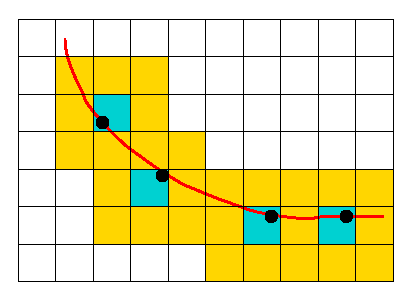
\includegraphics[width=0.4\linewidth]{images/selectB.eps} \\
(a) & (b)
\end{tabular}

\caption{2D illustration of vertex and cube selection.
(a) Selection which gives poor cover of the red curve.
The curve intersects an uncovered square.
(b) Selection which gives better cover of the red curve.
The curve is far away from any uncovered square.
}
\label{fig:select}
\end{figure}

\section{MergeSharp}

As show in Figure~\ref{alg:mergesharp}, Algorithm SHREC has three parts:
computation of isosurface vertex locations, 
selection of a well-spaced subset of vertices on sharp features
and merging of vertices around selected vertices.
Algorithm MergeSharp has a similar three parts,
but each part is substantially improved in SHREC.
We start with a brief description of MergeSharp
as presented in~\cite{bw-cisec-13}.

The computation of isosurface vertex locations
was described in Section~\ref{section:loc}.
The procedure in Section~\ref{section:loc}
returns not only a point $p_\cb$ on the isosurface,
but whether $p_\cb$ lies on a sharp corner, sharp edge or smooth portion 
of the isosurface.
Let $\Ccorner$ and $\Cedge$ be lists of cubes $\cb$ 
whose generated points $p_\cb$ lie on sharp corners and sharp edges, 
respectively.

As defined in Section~\ref{section:loc},
point $q_\cb$ is the centroid of interpolated intersection points
of the isosurface and grid edges of $\cb$.
Sort lists $\Ccorner$ and $\Cedge$ by increasing distance $|p_\cb - q_\cb|$
from $p_\cb$ to $q_\cb$.
Mark all the cubes as ``uncovered''.
Select the next uncovered cube $\cb$ in $\Ccorner$
where $p_\cb$ does not form a large angle triangle 
with vertices in previously selected cubes.
Merge $\cb$ with every uncovered vertex neighbor.
Mark all vertex neighbors of $\cb$ as covered.
The algorithm for $\Ccorner$ is shown in Figure~\ref{alg:select}.
After processing list $\Ccorner$, apply the same procedure to list $\Cedge$.

Note that the selection and merging are combined in the above description,
just as they are combined in~\cite{bw-cisec-13}.
In the modified version we present here,
those two steps will be separated.

There are problems with every one of the three steps of MergeSharp.
First, the vertex location $p_\cb$ generated by cube $\cb$
may lie outside $\cb$.
Moreover, point $p_\cb$ may lie outside of $\cb$
even if the sharp edge containing $p_\cb$ intersects $\cb$.
In addition, because of curvature, noise and numerical instability,
point $p_\cb$ could lie in some cube $\cb'$ adjacent to $\cb$
while point $p_{\cb'}$ lies inside $\cb$.
We will modify MergeSharp to generate point $p_\cb$ inside cube $\cb$
wherever possible.

Second, the selection step chooses cubes based on the proximity
of $p_\cb$ to $q_\cb$.
If a point $p_\cb$ is near $q_\cb$, 
it probably is located in cube $\cb$ 
and is a good approximation of the vertex location.
While this is reasonable,
it ignores the interaction between selected cubes.
MergeSharp does better when sharp edges are well-covered 
by the selected and covered cubes.
For instance, in the 2D illustration in Figure~\ref{fig:select}, 
the selected squares are packed together more closely
and their $3 \times 3$ regions do a better job of covering
the given curve.
We modified the MergeSharp selection to pack selected cubes 
more closely together.

Finally, the merging step merges cube $\cb$
with the the first selected cube adjacent to $\cb$.
Doing so sometimes distorts triangles, creating extremely thin triangles
and sometimes creating ``folds'' in the surface mesh.
We modify MergeSharp so that it prefers merging cubes which are facet
adjacent over merging edge adjacent or vertex adjacent cubes.
We add checks which avoid merging which creates small thin triangles
or creates folds.
We also extend the merging by one more cube in certain regions
to ensure good covering of sharp isosurface edges.


\begin{figure}[t]
\centering

\begin{tabular}{cc}
\includegraphics[width=0.4\linewidth]{images/centroid.eps} \qquad &
\qquad
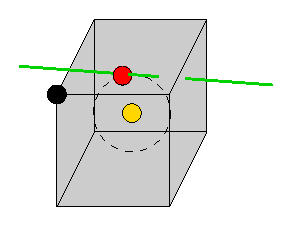
\includegraphics[width=0.4\linewidth]{images/center.eps} \\
(a) & (b)
\end{tabular}

\caption{The green line is the line containing the
sharp edge near cube $\cb$. 
Black cube vertices have scalar value above the isovalue.
(a) Green line intersects cube $\cb$
but point location $p^0_\cb$ (red) is outside cube $\cb$.
Cyan points are the intersection points of the isosurface
and the cube edges, computed using linear interpolation.
Gold point is $q_\cb$, the centroid of the cyan points, .
Red point is the closest point on the green line to $q_\cb$.
(b) Green line intersects cube $\cb$
but point location $p^1_\cb$ (red) is outside cube $\cb$.
Gold point is $\cb.\protect\Center$, the cube center.
Red point is the closest point on the green line to $\cb.\protect\Center$.
}
\label{fig:out_of_cube}
\end{figure}

\section{Generating Points on Sharp Features}
\label{section:generation}

\subsection{Computing Vertex Locations on Sharp Edges}

Consider an edge cube $\cb$.
By definition, edge cube $\cb$ is near some sharp edge.
The location $\cb.\isovLoc$ of the isosurface vertex associated with $\cb$ 
should be on that sharp edge.
However, that condition still gives one degree of freedom in selecting
the location of $\cb.\isovLoc$.
One obvious additional condition is that if the sharp edge intersects $\cb$,
then $\cb.\isovLoc$ should be in $\cb$.
An additional condition is that if the sharp edge does not intersect $\cb$,
then $\cb.\isovLoc$ should be ``close to'' $\cb$ 
under some suitably defined metric.

Algorithm SHREC computes three different possible isosurface vertex locations.
First, Algorithm SHREC computes $p^0_\cb$ 
by computing a line $L$ through the sharp edge and 
selecting the point on $L$ nearest the centroid point $q_\cb$.
Equation~\ref{eqn:Lindstrom}, for computing $p^0_\cb$ is given
in Section~\ref{section:loc}.
The idea is that the centroid point $q_\cb$ is a good approximation
for the intersection of $\cb$ and the isosurface,
and so one should choose a point near $q_\cb$.
If $p^0_\cb$ lies in $\cb$, then SHREC sets $\cb.\isovLoc$ to $p^0_\cb$.

In most cases, if line $L$ intersects cube $\cb$.
then the point $p^0_\cb$ will lie in $\cb$.
However, if line $L$ is ``near'' some facet or edge of $\cb$,
then it is possible for $L$ to intersect $\cb$ but $p^0_\cb$ to lie
outside $\cb$.
(See Figure~\ref{fig:out_of_cube}(a).)

If $p^0_\cb$ lies outside $\cb$,
then let $p^1_\cb$ be the point on $L$ which lies closest 
to the center $\cb.\Center$ of cube $\cb$.
We can compute $p^1_\cb$ replacing $q_\cb$ by $\cb.\Center$
in Equation~\ref{eqn:Lindstrom}.
If $p^1_\cb$ is in $\cb$ while $p^0_\cb$ is not,
SHREC sets $\cb.\isovLoc$ to $p^1_\cb$.

Unfortunately, it is possible that both $p^0_\cb$ and $p^1_\cb$ 
are not in $\cb$ even though $L$ intersects $\cb$.
(See Figure~\ref{fig:out_of_cube}(b).)
As a final step, we compute the point $p^2_\cb$ on $L$ which is closest 
to the center $\cb.\Center$ of $\cb$ under the $L_\infty$ metric.
If $L$ intersects $\cb$, then this point is guaranteed to lie in $\cb$.
Details for computing $p^2_\cb$ are in Appendix~\ref{appendix:Linf}.
If $p^2_\cb$ is in $\cb$ while $p^0_\cb$ and $p^1_\cb$ are not,
SHREC sets $\cb.\isovLoc$ to $p^2_\cb$.

Instead of computing $p^0_\cb$, $p^1_\cb$ and $p^2_\cb$, 
we could compute and use only $p^2_\cb$.
However, the computations of $p^0_\cb$ and $p^1_\cb$ are much faster,
and their locations are preferable to $p^2_\cb$ when they are
contained in cube $\cb$.
Algorithm MergeSharp computes only $p^0_\cb$.

\begin{figure}[t]
\centering

\begin{tabular}{cc}
\includegraphics[width=0.4\linewidth]{images/shared_edge.eps} \qquad &
\qquad
\includegraphics[width=0.4\linewidth]{images/shared_edge_B.eps} \\
(a) & (b)
\end{tabular}

\caption{(a) Two grids cubes sharing an edge $\eb$.
(b) The two other cubes (gold) which also contain $\eb$.
}
\label{fig:shared_edge}
\end{figure}

\begin{figure}[t]
\centering

\begin{tabular}{cc}
\includegraphics[width=0.4\linewidth]{images/shared_vertex.eps} \qquad &
\qquad
\includegraphics[width=0.4\linewidth]{images/shared_vertex_B.eps} \\
(a) & (b)
\end{tabular}

\caption{(a) Two grids cubes sharing a vertex $v$.
(b) The six other cubes (gold) which also contain $v$.
}
\label{fig:shared_vertex}
\end{figure}

\subsection{Swapping Locations}

Many of the problems in Algorithm SHREC (and MergeSharp) occur when
isosurface vertex location $\cb.\isovLoc$ lies outside of cube $\cb$.
Thus, it is always preferable that $\cb.\isovLoc$ be in $\cb$.
This is not always possible since the sharp edge or corner near $\cb$
may not intersect $\cb$.
However, in cases where a sharp edge or corner intersects $\cb$,
we would like $\cb.\isovLoc$ to be in $\cb$.

The computation of a sharp edge or corner near $\cb$ depends
upon gradients in the neighborhood of $\cb$.
The set of such gradients changes for each cube $\cb$.
Because of the inaccuracy in computing sharp edges and corners,
it is possible that $\cb.\isovLoc$ is in a cube $\cb'$ adjacent to $\cb$
while $\cb'.\isovLoc$ is not contained in $\cb$.
In some cases,
location $\cb.\isovLoc$ is in $\cb'$ while $\cb'.\isovLoc$ is in $\cb$.
In those cases,
we simply swap $\cb.\isovLoc$ and $\cb'.\isovLoc$.
In other cases, location $\cb'.\isovLoc$ lies in some third cube $\cb''$.
In that case, we simply set $\cb'.\isovLoc$ to $\cb.\isovLoc$.

The setting of isosurface vertex locations from adjacent cubes
increases the number of cubes $\cb$ containing 
their associated vertext locations $\cb.\isovLoc$.
Note that if the initial location $\cb.\isovLoc$ lies in $\cb$,
then we never change $\cb.\isovLoc$.


\begin{figure}
\centering
\begin{tabular}{cc}
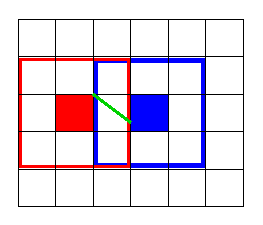
\includegraphics[width=1.2in]{images/config2D_2_0.eps} \qquad &
\qquad
\includegraphics[width=1.2in]{images/config2D_3_0.eps} \\
(a) Configuration (2,0). & (b) Configuration (3,0). \\
\\
\includegraphics[width=1.2in]{images/config2D_2_1.eps}
\qquad &
\qquad
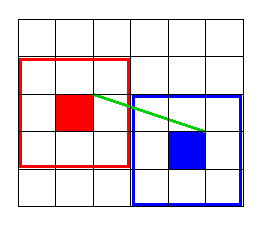
\includegraphics[width=1.2in]{images/config2D_3_1.eps} \\
(c) Configuration (2,1). & (d) Configuration (3,1).
\end{tabular}
\caption{Tightly packed 2D configurations of selected squares.
Selected squares and $3 \times 3$ region around each square.
Line segments with endpoints on the two selected squares 
(e.g., the green line segments) are contained
within the union of the two $3 \times 3$ regions.}
\label{fig:packed2D}
\end{figure}

\begin{figure}[t]
\centering
\begin{tabular}{cc}
\includegraphics[width=1.2in]{images/config2D_3_2.eps} \qquad &
\qquad
\includegraphics[width=1.2in]{images/config2D_2_2.eps} \\
(a) Configuration (3,2). & (b) Configuration (2,2). 
\end{tabular}
\caption{Problematic 2D configurations of selected squares.
Selected squares and $3 \times 3$ region around each square.
(a) The green line segment is not contained within the union
of the two $3 \times 3$ regions.
(b)~The green line segment intersects the boundary
of the union of the two $3 \times 3$ regions.}
\label{fig:loose2D}
\end{figure}

\begin{figure}[t]
\centering
\begin{tabular}{cc}
\includegraphics[width=1.2in]{images/config2D_4_2.eps} \qquad &
\qquad
\includegraphics[width=1.2in]{images/config2D_4_2_B.eps} \\
(a) Configuration (4,2). & (b) Additional cube.
\end{tabular}
\caption{(a) Configuration (4,2) has space between the $3 \times 3$
regions around each selected square.
(b) Additional cube (magenta) which packs tightly with two other squares.}
\label{fig:config2D_4_2}
\end{figure}

\begin{figure*}
\centering
\begin{tabular}{cccc}
\includegraphics[width=1.2in]{images/config3D_2_0_0.eps} \qquad &
\qquad
\includegraphics[width=1.2in]{images/config3D_3_0_0.eps}
\qquad &
\qquad
\includegraphics[width=1.2in]{images/config3D_2_1_0.eps}
\qquad &
\qquad
\includegraphics[width=1.2in]{images/config3D_3_1_0.eps} \\
(a) Configuration (2,0,0). & (b) Configuration (3,0,0). 
  & (c) Configuration (2,1,0). & (d) Configuration (3,1,0).
\end{tabular}
\caption{Tightly packed 3D configurations of selected cubes.}
\label{fig:packed3D}
\end{figure*}

\begin{figure*}
\centering
\begin{tabular}{ccc}
\includegraphics[width=1.2in]{images/config3D_3_2_0.eps} \qquad &
\qquad
\includegraphics[width=1.2in]{images/config3D_3_2_1.eps}
\qquad &
\qquad
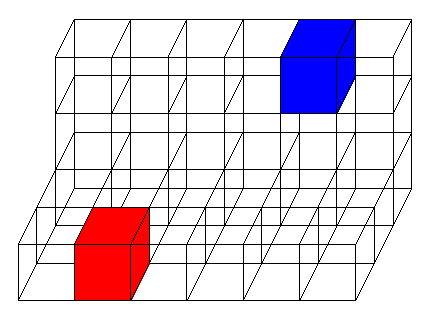
\includegraphics[width=1.2in]{images/config3D_3_2_2.eps} \\
(a) Configuration (3,2,0). & (b) Configuration (3,2,1). 
  & (c) Configuration (3,2,2).
\end{tabular}
\caption{Problematic 3D configurations of selected cubes.}
\label{fig:loose3D}
\end{figure*}

\begin{figure}[t]
\centering

\includegraphics[width=1.2in]{images/config3D_3_2_2_B.eps}

\caption{Problematic interaction of red and blue cubes
in configuration (3,2,2) is blocked by magenta cube.}
\label{fig:blocked3D}
\end{figure}

\subsection{Locations on Planes}

Consider two grid cubes, $\cb$ and $\cb'$, 
which intersect in an edge $\eb$ but not in any facet.
(See Figure~\ref{fig:shared_edge}.)
Two other grid cubes, $\tcb$ and $\tcb'$ share edge $\eb$.
A sharp edge which passes through $\cb$ and $\cb'$ must intersect
either $\tcb$ or $\tcb'$.
(In the exceptional case, the edge passes through $\eb$,
in which case it intersects both $\tcb$ and $\tcb'$.)
Since the edge intersects either $\tcb$ and $\tcb'$,
either $\tcb.\isovLoc$ should be in $\tcb$ 
or $\tcb'.\isovLoc$ should be in $\tcb'$.
However, because of inaccuracies in computing sharp edges and corners,
neither condition may hold.

To ensure that either $\tcb.\isovLoc$ lies in $\tcb$
or $\tcb'.\isovLoc$ lies in $\tcb'$,
Algorithm SHREC computes the plane $h$ containing $\eb$
and perpendicular to the line from $\cb.\Center$ to $\cb'.\Center$.
SHREC then computes the intersection of the line $L$ containing $\eb$
and plane $h$.
This intersections point, $p_I$, lies in either $\tcb$ or $\tcb'$.
If $p_I$ lies in $\tcb$ and $\tcb.\isovLoc$ is not in $\tcb$,
SHREC sets $\tcb.\isovLoc$ to $p_I$.
If $p_I$ lies in $\tcb'$ and $\tcb'.\isovLoc$ is not in $\tcb'$,
SHREC sets $\tcb'.\isovLoc$ to $p_I$.

Next consider the case of two grid cubes, $\cb$ and $\cb'$, 
which intersect in a vertex $v$ but not in any edge.
(See Figure~\ref{fig:shared_vertex}.)
Six other grid cubes share vertex $v$ with $\cb$ and $\cb'$.
A sharp edge which passes through $\cb$ and $\cb'$ must intersect
one of these six other grid cubes.
(In the exceptional case, the edge passes through $v$,
in which case all six.)
Since the edge intersects one of the six grid cubes,
point $\tcb.\isovLoc$ should lie in $\tcb$ for one of the six grid cubes $\tcb$.
Again because of inaccuracies in computing sharp edges and corners,
point $\tcb.\isovLoc$ may not be in $\tcb$ for any of the six grid cubes $\tcb$.

To ensure that $p_\tcb$ lies in $\tcb$ for one of the six grid cubes,
Algorithm SHREC computes the plane $h$ containing $v$
and perpendicular to the line from $\cb.\Center$ to $\cb'.\Center$.
SHREC then computes the intersection of the line $L$ containing $\eb$
and plane $h$.
This intersections point, $p_I$, lies in at least one of the six grid cubes.
If $p_I$ lies in cube $\tcb$ and $\tcb.\isovLoc$ is not in $\tcb$,
SHREC sets $\tcb.\isovLoc$ to $p_I$.

The computation in this section ensures ``continuity'' in the cubes
which intersect a sharp edge.
If a sharp edge intersects a cube $\cb$,
then the edge should intersect two cubes $\cb'$ and $\cb''$
which share a facet with $\cb$.
SHREC's computation of edge-plane intersections described above,
ensures that if $\cb'$ and $\cb''$ are active cubes,
then $\cb'$ will contain $\cb'.\isovLoc$ and 
$\cb''$ will contain $\cb''.\isovLoc$.


\section{Selecting Edge and Corner Cubes}
\label{section:selection}

Algorithm SHREC selects a well-spaced subset of the edge and corner cubes
and merges isosurface vertices adjacent cubes 
with the vertices generated by the selected cubes.
To ensure that the isosurface vertices on sharp features are well-spaced,
SHREC never selects two cubes which have a common vertex.
Whenever SHREC selects a cube $\cb$,
any adjacent cube sharing a vertex with $\cb$ is marked as ``covered''
by $\cb$.
SHREC never selects a covered cube.

As noted in Section~???, 
SHREC does better when selected cubes 
are packed ``tightly'' together.
In particular, SHREC tries to avoid certain configurations of nearby cubes.

Consider cubes $\cb$ and $\cb'$ with grid indices $(x_0,x_1,x_2)$
and $(x'_0,x'_1,x'_2)$, respectively.
(A cube with grid indices $(x_0,x_1,x_2)$ is in column $x_0$, row $x_1$
and $z$-plane $x_2$ of the grid.)
The {\em distance vector} between the cubes is
$(|x_0-x'_0|, |x_1-x'_1|, |x_2-x'_2|)$.
Two grid cubes are in configuration $(a_0,a_1,a_2)$ if the distance vector
between the cubes is some permutation of $(a_0,a_1,a_2)$.
Figures~\ref{fig:packed2D}, \ref{fig:loose2D}, \ref{fig:config2D_4_2}
and~\ref{fig:packed3D},
contain examples of 2D and 3D configurations of grid cubes.

We can get some insight into 3D configurations of grid cubes
by considering the 2D configurations of grid squares.
Figure~\ref{fig:packed2D} contains configurations $(2,0)$, $(3,0)$,
$(2,1)$ and $(3,1)$ of grid squares.
The $3 \times 3$ regions around the selected squares are ``tightly packed''
so that any line segment with endpoints in the selected squares
is contained within the union of the two $3 \times 3$ regions.

Figure~\ref{fig:loose2D} contains configurations $(3,2)$ and $(2,2)$
of grid squares.
With configuration $(3,2)$, some line segments with endpoints
in the selected squares are not contained within the union
of the $3 \times 3$ regions.
Configuration $(2,2)$ is somewhat better,
since all line segments with endpoints in the selected squares
are contained within the union of the $3 \times 3$ regions.
Unfortunately, they are only barely contained.
The green line segment in Figure~\ref{fig:loose2D}(b) intersects
the boundary of the $3 \times 3$ region.
Slightly curving the segment could mean that it no longer was contained
in the union.

Note that if selected squares are suitably far apart,
then additional squares can be selected between them.
For instance, a magenta square can be selected between the two colored squares
in Figure~\ref{fig:config2D_4_2}(a) and the $3 \times 3$ regions
will fit together tightly.

Some examples of tightly packed 3D configurations of cubes are given
in Figure~\ref{fig:packed3D}.
Any line segment with endpoints in the two selected cubes $\cb$ and $\cb'$
will be well contained within the union 
of the two $3 \times 3 \times 3$ regions, 
$\RIII_\cb$ and $\RIII_{\cb'}$, around $\cb$ and $\cb'$.

Figure~\ref{fig:loose3D} contains three problematic configurations,
$(3,2,0)$, $(3,2,1)$ and $(3,2,2)$,
of  selected cubes.
Line segments with endpoints in the two selected cubes $\cb$ and $\cb'$
may contain points outside $\RIII_\cb \cup \RIII_{\cb'}$.
SHREC attempts to avoid selecting cubes with these configurations.

If two selected cubes, $\cb$ and $\cb'$, 
are in configuration $(2,2,0)$, $(2,2,1)$ or $(2,2,2)$,
then a line segment with endpoints in $\cb$ and $\cb'$
could intersect the boundary of $\RIII_\cb \cup \RIII_{\cb'}$.
Such configurations are undesirable.
Unfortunately, we found that avoiding such configurations is too restrictive.

Consider two cubes, $\cb$ and $\cb''$ 
in a $(3,2,0)$, $(3,2,1)$ or $(3,2,2)$ configuration.
If a third selected cube $\cb'$ lies between $\cb$ and $\cb''$,
then the sharp edge will pass from $\cb$ to $\cb'$ to $\cb''$.
The selection of $\cb'$ ``blocks'' the problematic interaction 
of $\cb$ and $\cb''$.
If cubes $\cb$ and $\cb'$ are selected,
then SHREC will permit the selection of $\cb''$,
even though $\cb$ and $\cb''$ have a configuration $(3,2,*)$.
Figure~\ref{fig:blocked3D} contains an example of two cubes 
in a $(3,2,2)$ configuration and a third cube between them.

More formally,
let $\cb$, $\cb'$ and $\cb''$ be grid cubes with grid indices
$(x_0,x_1,x_2)$, $(x'_0,x'_1,x'_2)$ and $(x''_0,x''_1,x''_2)$, respectively.
Cube $\cb'$ {\em separates} $\cb$ from $\cb''$
if $x'_i \in [x_i,x''_i]$ for $i = 0,1,2$
and $x_i < x'_i < x''_i$ or $x_i > x'_i > x''_i$ for some $i$.
SHREC avoids selecting cube $\cb''$ if some already selected cube $\cb$
forms a $(3,2,0)$ or $(3,2,1)$ or $(3,2,2)$ configuration with $\cb''$
and no already selected cube separates $\cb$ from $\cb''$.

SHREC first selects corner cubes.
When the corner location is inside an active cube,
SHREC selects the active cube containing the corner.
When the corner location is not in an active cube,
SHREC selects the active cube ``closest'' to the corner location
by choosing the cube whose center has minimum $L_\infty$ distance
to the corner.

SHREC next selects edge cubes which are ``near'' the corner cubes,
i.e., they are contained in an $7 \times 7 \times 7$ region
around each corner cube.
Selecting edge cubes near corners poses special challenges
since there are multiple sharp edges ending at a corner.
Selecting a cube which is near two such sharp edges
can obscure one of the edges.

Let $\cb$ be a corner cube and let $\cb'$ be an edge cube
which is in a $(2,0,0)$, $(2,1,0)$ or $(2,1,1)$ configuration with $\cb$.
Let $\cb''$ be any cube sharing an edge or facet with $\cb'$
which is contained in the $5 \times 5 \times 5$ region
but is not covered by $\cb$.
If $\cb''$ is active and an edge cube,
then SHREC attempts to avoid selecting cube $\cb'$.

Once edge cubes near corners are selected,
SHREC could iterate by selecting uncovered edge cubes 
near already selected cubes.
If no uncovered edge cubes were near selected cubes,
SHREC could select an arbitrary uncovered edge cube
and extend the set of selected cubes from that cube.
By not selecting a cube $\cb''$ 
if it forms a $(3,2,0)$, $(3,2,1)$ or $(3,2,2)$
with an already selected cube $\cb$ 
(and is not separated by a selected cube from $\cb$,)
SHREC would produce a tight packing of selected cubes.

The algorithm outlined in the previous paragraph would produce
a good set of selected cubes but it is highly sequential.
One of the best aspects of the Marching Cubes and dual contouring algorithms
is their local, distributed, paralellizable nature.
Sequentially extending the set of selected cubes would totally destroy
that aspect of the algorithms.
Instead of selecting cubes using the sequential algorithm given above,
SHREC divides the regular grid 
into overlapping $6 \times 6 \times 6$ regions,
selects cubes from the boundaries of those regions and then from their interior.
The algorithm is completely local and easily distributed and parallelizable.

Each grid cube has an index $(x_0, x_1, x_2)$.
SHREC processes the grid cubes by reducing the indices modulo six
to $(x_0 \bmod 6, x_1 \bmod 6, x_2 \bmod 6)$.
SHREC first selects edge cubes with indices congruent to $(0,0,0)$ modulo six.
SHREC next selects edge cubes with indices congruent modulo six
to $(\pm 1,0,0)$ or $(0, \pm 1, 0)$ $(0, 0, \pm 1)$.
SHREC then selects edge cubes with indices congruent modulo six
to $(\pm 2,0,0)$ or $(0, \pm 2, 0)$ $(0, 0, \pm 2)$.
Finally, SHREC selects edge cubes with indices congruent modulo six
to $(3,0,0)$ or $(0, 3, 0)$ $(0, 0, 3)$.
SHREC does not select an edge cube $\cb$ if some already selected cube $\cb'$
forms configuration $(3,2,0)$, $(3,2,1)$ or $(3,2,2)$ with $\cb$
and no already selected cube separates $\cb$ from $\cb''$.

SHREC next selects edge cubes which are some permutation
of $(k_a,k_b,0)$ modulo six,
starting first with permutations of $(\pm 1, \pm 1, 0)$
and ending with permutations of $(3, 3, 0)$.
Finally, SHREC selects edge cubes which are permutations
$(k_a, k_b, k_c)$ modulo six,
starting first with permutations of $(\pm 1, \pm 1, \pm 1)$
and ending with $(3, 3, 3)$.

It is possible that the selection of two edge cubes $\cb$ and $\cb''$
at distance five apart can force the selection of an edge cube $\cb'$
which has a $(3,2,1)$ or $(3,2,2)$ configuration 
with either $\cb$ or $\cb''$.
This happens if the distance vector between $\cb$ and $\cb''$
is $(5,3,2)$.
Thus, in addition to avoiding $(3,2,*)$ configurations,
SHREC also avoids selecting two cubes, $\cb$ and $\cb''$, 
which form a $(5,3,2)$ configuration.
Of course, if $\cb$ and $\cb''$ are separated by some other selected cube,
then they can both be selected.

While the above rules select a set of cubes which almost completely cover
the sharp edges of a surface,
it is possible that the configuration restrictions leave a few areas uncovered.
Therefore, SHREC repeats the selection process to select any remaining
uncovered edge cubes but drops the configuration restrictions.


\section{Merging Points with Features Points}
\label{section:merging}

Algorithm MergeSharp merges neighbors of a selected cube $\cb$ 
with $\cb$ when $\cb$ is selected.
This merging step sometimes created extremely thin triangles and 
sometimes flips triangle orientations.
SHREC is much more careful about its cube merging.
SHREC also extends the merging to some cubes in a $5 \times 5 \times 5$ region 
around each selected cube.
Note that SHREC actually merges the isosurface vertices generated by the cubes,
not the cubes themselves.

SHREC relies upon some angle tests to determine permissible merging.
Before performing such tests, SHREC maps the grid 
and the computed isosurface locations $\cb.\isovLoc$
to the regular grid composed of unit cubes.

\subsection{Ordered Merging}
\label{section:ordered_merging}

SHREC first merges neighbors of selected corner cubes.
SHREC merges these neighbors in three steps.
First, for each selected corner cube $\cb$,
SHREC merges with $\cb$ the active cubes which share a facet with $\cb$.
Next, for each selected corner cube $\cb$,
SHREC merges with $\cb$ the active cubes which share an edge with $\cb$.
Finally, for each selected corner cube $\cb$,
SHREC merges with $\cb$ the active cubes which share a vertex with $\cb$.
Of course, once an active cube is merged with some selected cube,
it is never merged with any other cube.

SHREC next merges neighbors of selected corner cubes.
The procedure is similar to the one for corner cubes.
SHREC first merges active cubes which share a facet with a selected edge cube,
then merges active cubes which share an edge with a selected edge cube,
and finally merges active cubes which share a vertex 
with a selected edge cube.

\subsection{Merging Tests}
\label{section:merging_tests}

For both the corner cube and edge cube merging,
SHREC applies five different tests to avoid creating very thin triangles
or flipping triangles or violating manifold conditions.
Consider a cube $\tcb$ which SHREC would like to merge 
with a selected cube $\cb$.
First, SHREC checks that the isosurface vertex in $\tcb$
is connected to the isosurface vertex in $\cb$.
A cube $\tcb$ is connected to a selected cube $\cb$
if $\tcb$ shares an active facet with $\cb$
or some cube $\tcb'$ shares an active facet with $\tcb$ and
is merged with $\cb$.
(A facet is active if some facet vertex has scalar value greater than
or equal to the isovalue and some facet vertex has scalar value less
than the isovalue.)
If $\tcb$ is not connected with $\cb$, then $\tcb$ is not merged with $\cb$.

Second, SHREC checks for some manifold violations that
could be caused by merging $\tcb$ with $\cb$.
For each such selected cube $\cb' \neq \cb$ which is connected to $\tcb$,
SHREC checks if $\cb'$ is connected to $\cb$.
Let $\cb'$ be a selected cube which is connected to $\cb$ and $\tcb$.
Each active edge $\eb$ of $\tcb$ is dual to an isosurface quadrilateral
with a vertex in $\tcb$.
Let $\tcb_1$, $\tcb_2$, and $\tcb_3$ be the three other cubes containing $\eb$.
If some $\tcb_i$ merges with $\cb$ and another $\tcb_j$ merges with $\cb'$,
then merging $\tcb$ with $\cb$ collapses this quadrilateral to a triangle
or an edge.
However, if no isosurface quadrilateral dual to an active edge of $\tcb$
has vertices in $\tcb$, $\cb$ and $\cb'$,
then merging $\tcb$ with $\cb$ creates a non-manifold edge 
from $\cb$ to $\cb'$ with four incident polygons.
If some selected $\cb'$ is connected to both $\cb$ and $\tcb$,
but no isosurface quadrilateral has vertices in $\tcb$, $\cb$ and $\cb'$,
then SHREC does not merge $\tcb$ with $\cb$.

Third, SHREC checks whether mapping $\tcb$ to $\cb$
will create thin triangles between selected cubes.
If SHREC is connected to selected edge cubes $\cb$, $\cb'$ and $\cb''$
and $\cb''$ lies between $\cb$ and $\cb'$
(or $\cb'$ lies between $\cb$ and $\cb''$),
then mapping $\tcb$ to $\cb$ will create a thin triangle
with vertices in $\cb$, $\cb'$ and $\cb''$.
Let $\cb$, $\cb'$ and $\cb''$ be grid cubes with grid indices
$(x_0,x_1,x_2)$, $(x'_0,x'_1,x'_2)$ and $(x''_0,x''_1,x''_2)$, respectively.
If $(x''_0,x''_1,x''_2)$ is contained in the box with corners
$(x_0,x_1,x_2)$ and $(x'_0,x'_1,x'_2)$ and does not lie on any 
of the eight corners of that box,
then we say that $\cb''$ lies between $\cb$ and $\cb'$.
If $\tcb$ is connected to selected edge cubes $\cb$, $\cb'$ and $\cb''$,
and $\cb''$ lies between $\cb$ and $\cb'$,
then SHREC does not merge $\tcb$ with $\cb$.

Fourth, SHREC checks whether mapping $\tcb$ creates thin triangles
or flips triangles.
This test is described in Section~\ref{section:distortion_tests}.

Finally, SHREC checks whether cube $\tcb$ has more than one isosurface vertex.
If cube $\tcb$ has more than one isosurface vertex,
then it has at least one ambiguous facet.
(A facet is ambiguous if two diagonally opposite vertices have
scalar value above the isovalue while the other two vertices
have scalar value below the isovalue.)
Let $\tcb'$ be a cube sharing an ambiguous facet with $\tcb$.
If cube $\tcb$ has only one isosurface vertex and 
$\tcb'$ is not merged with $\cb$, then $\tcb$ is not merged with $\cb$.

\subsection{Distortion Tests}
\label{section:distortion_tests}

Let $q$ be a quadrilateral dual to some active edge of $\tcb$.
Let $\tw$ be the vertex of $q$ which is generated by $\tcb$.
Quadrilateral $q$ can either be triangulated by adding a diagonal
incident on $\tw$ or by adding a diagonal connecting the neighbors
of $\tw$ in $q$.
Triangulating $\tw$ by adding a diagonal incident on $\tw$
places more restrictions on possible locations of $\tw$.
Since SHREC does not know how $q$ will be triangulated,
it assumes this more restrictive triangulation.

The diagonal of $q$ incident on $\tw$ splits $q$ into two triangles.
SHREC checks whether mapping $\tcb$ to $\cb$ will severely distort
either of those triangles.
Let $\tcb$, $\tcb'$ and $\tcb''$ be the cubes 
containing the triangle vertices.
SHREC only checks triangles where $\tcb'$ and $\tcb''$ 
are not covered or selected.

Let $\tw$, $\tw'$ and $\tw''$ be the vertices generated
by $\tcb$, $\tcb'$ and $\tcb''$.
Let $w$ be the vertex generated by selected cube $\cb$.
SHREC applies three tests to determine if mapping $\tw$ to $w$
severely distorts triangle $(\tw,\tw',\tw'')$.
The first test simply checks that the angles in the new triangle
are not very small.
If $\angle(w,\tw',\tw'')$ or $\angle(w,\tw'',\tw')$ is less than $5^\circ$,
then SHREC does not map $\tcb$ to $\cb$.

The second test checks whether mapping $\tw$ to $w$
significantly changes the normal of triangle $(\tw,\tw',\tw'')$.
If the angle between the normal of $(w, \tw', \tw'')$ is less than $30^\circ$,
then the triangle passes this test.

The third test checks the orientation of $(w, \tw', \tw'')$.
Let $\eb$ be the grid edge shared by cubes $\tcb$, $\tcb'$ and $\tcb''$.
Let $\pi(w)$, $\pi(\tw')$ and $\pi(\tw'')$ be the orthogonal projection
of $w$, $\tw'$ and $\tw''$, respectively, 
onto a plane $h$ perpendicular to $\eb$.
If the orientation of $\pi(w)$, $\pi(\tw')$ and $\pi(\tw'')$
matches the orientation of $\tcb$, $\tcb'$ and $\tcb''$ around $\eb$,
then triangle $(w,\tw',\tw'')$ passes the orientation test.

We require that a triangle pass either the normal or the orientation test,
not necessarily both test.
The original triangle $(\tw,\tw',\tw'')$ could have a normal which
is very far from the true surface normal.
In that case, we actually want the normal of triangle $(w, \tw', \tw'')$
to be far from the normal of triangle $(\tw, \tw', \tw'')$.
On the other hand,
the projected vertices $\pi(w)$, $\pi(\tw')$ and $\pi(\tw'')$
could be nearly collinear.
In that case, $\pi(w)$, $\pi(\tw')$ and $\pi(\tw'')$ could have
opposite orientation from $\tcb$, $\tcb'$ and $\tcb''$,
even though the normal of $(w,\tw',\tw'')$ is quite close
to the original.


\subsection{Pair Merging}
\label{section:pair_merging}

A cube $\tcb$ may fail to merge with a selected cube $\cb$
because of some neighboring cube $\tcb'$
while $\tcb'$ fails to merge with $\cb$ because of $\tcb$.
Often this ``deadlocking'' arises when $\tcb$ and $\tcb'$ share
a common ambiguous facet.

After attempting to merge individual cubes,
SHREC tries to merge pairs $(\tcb,\tcb')$ of covered cubes with selected cubes.
The elements of the pairs should share a common facet or edge
and should both be covered by the selected cube $\cb$.
SHREC temporarily merges $\tcb$ with $\cb$,
and then applies all the above tests to $\tcb'$.
SHREC then temporarily merges $\tcb'$ with $\cb$,
and applies all the above tests to $\tcb$.
If both $\tcb$ and $\tcb'$ pass the tests,
then SHREC merges both of them with $\cb$.

As the merging proceeds,
it is possible that a cube which was previously unable 
to merge with any selected cube
is now able to merge with some such cube.
Thus, SHREC reapplies the algorithm in Section~\ref{section:ordered_merging}
and in this section to any remaining covered, unmerged cubes.


\subsection{Extended Merging}
\label{section:extended_merging}

The merging of cubes in $3 \times 3 \times 3$ region
around each selected cube will clear most but not all of the vertices 
around sharp edges and corners.
There are multiple reasons that some vertices near sharp edges may remain.
First, the location of some vertex outside of $\RIII_\cb$
may stop some cube covered by $\cb$ from merging with $\cb$.
Second, if two selected $\cb$ and $\cb'$ are 
in a $(2,2,0)$ or $(2,2,1)$ or $(2,2,2)$ configuration, 
then a sharp edge with endpoints in $\cb$ and $\cb'$ can intersect
the boundary of the $\RIII_\cb \cup \RIII_{\cb'}$.
Vertices in uncovered can be arbitrarily close to such a sharp edge.
Third, while the selection step avoids most $(3,2,*)$ configurations,
it does not avoid all of them.
If $\cb$ and $\cb'$ are in a $(3,2,*)$ configurations,
then a sharp edge with endpoints in $\cb$ and $\cb'$ may contain points
outside of $\RIII_\cb \cup \RIII_{\cb'}$.

To handle such problems, SHREC extends the merging to cubes
in a $5 \times 5 \times 5$ region around each selected cube.
Merging cubes in a $5 \times 5 \times 5$ region $\RV_\cb$
around a selected cube $\cb$ can create its own problems 
of thin or flipped triangles.
Thus, SHREC only attempts to merge cubes in $\RV_\cb$
which are potentially near a sharp edge through $\cb$.

First, SHREC checks whether any covered cubes are unmerged
after the steps in Sections~\ref{section:ordered_merging}
and~\ref{section:pair_merging}.
If some cube $\tcb$ is covered by selected cube $\cb$
but not merged with any cube,
SHREC pairs $\tcb$ with any adjacent active cubes $\tcb'$
sharing a vertex with $\tcb$
and attempts to merge the pair $(\tcb,\tcb')$ with $\cb$.
SHREC applies the pair merging procedure
in Section~\ref{section:pair_merging} to determine whether
to allow the pair $(\tcb,\tcb')$ to merge with $\cb$.
Note that in Section~\ref{section:pair_merging} both cubes in the pair
must be contained in $\RIII_\cb$ while here only one cube
must be contained in $\RIII_\cb$.

It is possible that the interaction of vertices in three cubes
prevents a covered cube from merging with a selected cube.
SHREC considers triples of unmerged cubes
which share a common edge $\eb$.
At least one cube in the triple must be in $\RIII_\cb$.
The triple merging procedure is similar to the pair merging procedure
described in Section~\ref{section:pair_merging} and is omitted.

Next, SHREC tries to merge cubes which lie 
at the intersection $\partial \RIII_\cb \cap \RIII_{\cb'}$
of two $\gDim{3}$ regions around two selected cubes $\cb$ and $\cb'$.
More specifically, SHREC attempts to merge a cube $\tcb$ 
with a selected cube $\cb$ if some facet of $\tcb$ lies 
on the boundary of $\RIII_\cb$ 
while some other facet of $\tcb$ lies on the boundary of $\RIII_{\cb'}$.
Note that such a cube is contained in $\RV_\cb$.
SHREC applies all the tests in Section~\ref{section:merging_tests}
to determine whether to merge $\tcb$ with $\cb'$.

Finally, SHREC tries to merge pairs of cubes $(\tcb, \tcb')$ which lie
at the intersection $\partial \RIII_\cb \cap \RIII_{\cb'}$.
Both $\tcb$ and $\tcb'$ must have facets which lie on $\RIII_\cb$
and $\RIII_{\cb'}$.
SHREC applies the pair merging procedure described 
in Section~\ref{section:pair_merging} to determine whether
to allow the pair $(\tcb,\tcb')$ to merge with $\cb$.

\section{Selecting Gradients}
\label{section:gradients}

The algorithm in Section~\ref{section:loc}
for computing isosurface vertex locations requires
a set of gradients for each cube $\cb$.
An obvious set is the gradients at the vertices of $\cb$.
However, even if correct gradients were provided at every vertex of $\cb$,
this set would not suffice.
It is possible to have an active cube $\cb$
which contains a sharp isosurface corner
defined by three perpendicular planes
while only two of the planes are represented by the gradients of $\cb$.

MergeSharp computes isosurface vertex locations 
from the vertices of $\cb$ and of the six cubes sharing a facet with $\cb$.
When exact gradients are provided at all grid vertices,
this set of gradients suffices.

When gradients are not provided in the input,
they must be computed from the scalar data.
If an isosurface has sharp features,
then the gradient field is discontinuous around those sharp features.
As discussed in~???, 
computing correct gradients near gradient field discontinuities
is extremely difficult.
In~???, Bhattaca and Wenger give an algorithm for computing correct gradients
in the presence of gradient discontinuities, but the algorithm does
not compute correct gradients at all the grid vertices.
Instead, the algorithm returns a set of correct gradients
at some of the grid vertices while returning no gradient information
at other vertices.
Under suitable conditions,
the algorithm returns the correct gradient at any vertex
which is at least three edge lengths from any gradient discontinuity.

Because the algorithm in~??? does not return gradients 
near gradient discontinuities,
no gradient information may be available for the vertices 
of cubes which contain those discontinuities
or for neighbors of such cubes.
Thus, we must use gradients from a $\gDim{7}$ region around each cube $\cb$.

When scalar data is provided by computer tomography (CT),
then the scalar values near gradient discontinuities
may also be incorrect.
As discussed in~???, we must go out even further to a $\gDim{9}$ region 
around each cube $\cb$ to get gradient information.

Only gradients which determine isosurface tangent planes near $\cb$
should be used in $\cb.\isovLoc$.
We use three tests on the vertices in a $\gDim{7}$ or $\gDim{9}$
region around $\cb$ to determine such gradients.
First, we are only interested in vertices which are near the isosurface.
Thus, we only choose vertices from edges
where one endpoint has scalar value below
the isovalue and one endpoint has scalar value at or above the isovalue.
Second, we are only interested in vertices whose gradients generate planes
which are close to $\cb$.
We construct a cube $\cb'$ of size $1.5 \times 1.5 \times 1.5$ centered at $\cb$
and only choose a vertex $v$ 
if the plane $h_v$ given by Equation~\ref{eqn:isoplane}
intersects $\cb'$.

???

In smooth, curved surfaces, choosing gradients at vertices far from $\cb$
can cause the creation of non-existent sharp features in the isosurface.
Thus, we wish to only choose a vertex which is far from $\cb$
if the closer vertices are not chosen.

Let $Q$ be the set of vertices of the subgrid
whose gradients are $(0,0,0)$.
Let $Q_\cb$ be the vertices of $\cb$.
Let $G_\cb$ be the graph whose vertices are $Q \cup Q_\cb$
and whose edges are $(u,v)$ where $(u,v)$ is a grid edge.
We find the connected component $G'$ of $G_\cb$ containing $Q_\cb$.
A grid vertex $u \not\in V(G')$ is on the boundary of $G'$
if $(u,v)$ is a grid edge and $v$ is in $V(G')$.
We only a choose a vertex if it is in $Q_\cb$
or if it is on the boundary of $G'$.

Applying the three tests gives a set of vertices and their gradients
which define planes.
We use those vertices and their gradients to compute $p_\cb$
as described in Section~\ref{section:loc}.


\section{Parameters}
\label{section:parameters}

Algorithm SHREC has two major parameters,
one determining the number of large singular values in matrix $A$
and the second determining the size of the $\gDim{k}$ region 
from which gradients are selected around each cube
(Section~\ref{section:gradients}).
The first parameter is a value $\epsilon$ between 0 and 1.
As noted in Section~\ref{section:loc},
a singular value $\sigma_i$ of matrix $A$ 
is large if $\sigma_i/\sigma_1$ is greater than or equal to $\epsilon$.
The number of large singular values determines whether a vertex
is on a sharp corner or a sharp curve or a smooth region of the isosurface.
To the best of our knowledge, all algorithms which reconstruct surfaces 
with sharp corners or sharp curves require some parameter
to distinguish the corners and curves from the smooth regions of the surface.

The second parameter is an odd integer $k \ge 3$.
Each cube $\cb$ uses gradients from a $\gDim{k}$ around the cube
in selecting gradients for computing $\cb.\isovLoc$.
The size of $k$ depends upon the input data.
If correct gradients are provided at each grid vertex,
then $k$ should equal 3 for a $\gDim{3}$ region around each cube.
If gradients are computed from correct scalar values 
using the algorithm in~???,
then $k$ should equal 7 for a $\gDim{7}$ region around each cube.
If gradients are computed from CT data 
using the algorithm in~???,
then $k$ should equal 9 for a $\gDim{9}$ region around each cube.

SHREC uses three other constants:
one for the triangle test in selecting vertices,
one for the angle test in merging cubes
and a second for the normal test in merging cubes.
In the triangle test,
if selecting cube $\cb$ would possibly create a triangle between three
selected cubes with angle greater than $150^\circ$, 
cube $\cb$ is not selected.
In the angle test,
if merging cube $\tcb$ with $\cb$ would create a triangle with angle
less than $5^\circ$, then cube $\tcb$ is not selected.
In the normal test,
if merging $\tcb$ with $\cb$ would change the normal 
of some triangle $(\tw,\tw',\tw'')$ by less than $30^\circ$,
then merging $\tcb$ with $\cb$ does not distort triangle $(\tw,\tw',\tw'')$.

Because SHREC is based on the regular grid,
the constants used in all three of these tests do not depend 
upon the input data and should work well for any scalar fields.
Note that SHREC maps the input grid 
and the computed isosurface locations $\cb.\isovLoc$
to the regular grid composed of unit cubes
before applying any of the above tests.


\newcommand{\dAe}   {\ensuremath{d_A^\epsilon}}
\newcommand{\dApe}  {\ensuremath{d_A^{+\epsilon}}}
\newcommand{\tdAe}  {\ensuremath{\tilde{d}_A^\epsilon}}
\newcommand{\tdApe} {\ensuremath{\tilde{d}_A^{+\epsilon}}}
\newcommand{\triP}  {\ensuremath{\tau_P}}
\newcommand{\triQ}  {\ensuremath{\tau_Q}}
\newcommand{\triPP} {\ensuremath{\tau'_P}}
\newcommand{\triQQ} {\ensuremath{\tau'_Q}}

\begin{figure}[t]
\centering

\psfrag{A}{$A$}
\psfrag{Ap}{$A'$}
\psfrag{B}{$B$}
\psfrag{p}{$p$}
\psfrag{q}{$q$}

\begin{tabular}{cc}
\includegraphics[width=0.4\linewidth]{images/rectA.eps} \qquad &
\qquad
\includegraphics[width=0.4\linewidth]{images/rectAclose.eps} \\
(a) & (b) \\
\includegraphics[width=0.4\linewidth]{images/polyB.eps} \qquad &
\qquad
\includegraphics[width=0.4\linewidth]{images/polyBclose.eps} \\
(c) & (d)
\end{tabular}

\caption{(a) Rectangle $A'$ is a slight perturbation of rectangle $A$.
(b)~Close up view of dotted region around point $p$.
(c) The corner of polygon $B$ is clipped near $q$.
(d)~Close up view of dotted region around point $q$.}
\label{fig:rect}

\end{figure}


\section{Measuring Angular Distance between Surfaces}
\label{section:angular_distance}

As described in Section~\ref{section:related},
we evaluated MergeSharp in~\cite{bw-cisec-13}
by extracting sharp mesh edges (dihedral angle less than $140^\circ$)
and comparing the 1-skeleton formed
by those sharp edges with the 1-skeleton of the sharp edges 
in an ideal surface.
We present here a different way of evaluating 
a reconstructed mesh containing sharp features.

Let $\Sigma_P$ and $\Sigma_Q$ be two surfaces.
Given a point $p \in \Sigma_P$,
the distance, $d(p,\Sigma_Q)$, from $p$ to $\Sigma_Q$
is the distance from $p$ to the closest point on $\Sigma_Q$,
i.e., $d(p, \Sigma_Q) = min_{q \in \Sigma_Q} d(p,q)$.
We would like a similar measurement of the difference between
the normal at $p$ and the normals of $\Sigma_Q$.

The simplest approach would be to locate the point $q \in \Sigma_Q$
closest to $p$ and measure the difference 
between their normals.
As shown in Figure~\ref{fig:rect},
this measurement is not be very useful.
Rectangle $A'$ is a slightly translation of rectangle $A$.
The boundaries of rectangles $A$ and $A'$
are close under the Hausdorff metric and their normals are the same.
However, point $p$ is in the intersection of the two boundaries,
$\partial A$ and $\partial A'$,
but the normal to point $p$ in $\partial A$ is $90^\circ$
from the normal to point $p$ in $\partial A'$.
Furthermore, for any point $\tp \in A$ in a suitably small neighborhood of $p$,
the closest point in $\tp' \in A'$ has normal which is $90^\circ$
from the normal of $A$ at $\tp$.
Note that the translation could be arbitrarily small
and there would still be a point in $A$ whose normal was $90^\circ$
from the closest point in $A'$.

In contrast to the match between the normals of $A$ and $A'$, 
the corner of polygon $B$ in Figure~\ref{fig:rect}(c)
is clipped and its normal is $45^\circ$ from any normal of $A$.
We would like some measurement which gives a high value 
between $q \in B$ and $A$ while giving a low value between
any point of $A'$ and $A$.
Our idea is to compare the normal at $p \in \Sigma_P$ 
with the normals of $\Sigma_Q$ in some suitable neighborhood 
around $p$.

Let $\Sigma^S_P$ and $\Sigma^S_Q$ be the set of smooth points
in $\Sigma_P$ and $\Sigma_Q$.
Let $n_p$ and $n_q$ be the normals of $p \in \Sigma^S_P$
and $q \in \Sigma^S_Q$, respectively.
Let $B_p(\epsilon)$ be the ball around $p$ of radius $\epsilon$.
For each point $p \in \Sigma^S_a$ 
where $B_p(\epsilon) \cap \Sigma^S_Q \neq \emptyset$,
define the angle distance between $p$ and $\Sigma_Q$
in the neighborhood $\epsilon$ as:
\begin{align*}
\tdAe(p,\Sigma_Q) & = \liminf\{ \angle(n_p, n_q) : 
q \in \Sigma^S_Q \cap B_p(\epsilon) \}.
\end{align*}

Define the directed angle distance between $\Sigma_P$ and $\Sigma_Q$
in neighborhood $\epsilon$ as:
\begin{align*}
\tdAe(\Sigma_P,\Sigma_Q) & = 
  \limsup_{p \in \Sigma^S_P \mbox{ and } 
  B_p(\epsilon) \cap \Sigma^S_Q \neq \emptyset} 
         \tdAe(p,\Sigma_Q).
\end{align*}

Finally, define the angle distance between $\Sigma_P$ and $\Sigma_Q$
in neighborhood $\epsilon$ as:
\begin{align*}
\dAe(\Sigma_P,\Sigma_Q) & = 
\max(\tdAe(\Sigma_P,\Sigma_Q), \tdAe(\Sigma_Q,\Sigma_P)).
\end{align*}

The angle distance depends upon the parameter $\epsilon$.
If some point $p \in \Sigma^S_P$ is not within $\epsilon$ of $\Sigma_Q$,
then $\tdAe(p,\Sigma_Q)$ is undefined.
To address this problem, we replace the neighborhood $B_p(\epsilon)$
by an extended neighborhood $B_p(\epsilon+d(p,\Sigma_q))$
where $d(p,\Sigma_q)$ is the distance from $p$ to $\Sigma_Q$.
The ball around $p$ is now guaranteed to intersect $\Sigma_Q$.

Define the angle distance 
between $p \in \Sigma^S_p$ and $\Sigma_Q$ in the extended
neighborhood $\epsilon$ as:
\begin{align*}
\tdApe(p,\Sigma_Q) & = 
  \liminf\{ \angle(n_p, n_q) : 
     q \in \Sigma^S_Q \cap B_p(\epsilon+d(p,\Sigma_Q)) \}.
\end{align*}
As before, $d(p,\Sigma_Q)$ is the distance from $p$ to the closest point on $Q$.
Note that the addition of $d(p,\Sigma_Q)$ ensures that the ball
around $p$ intersects $\Sigma_Q$.

Define the directed angle distance between $\Sigma_P$ and $\Sigma_Q$
in extended neighborhood $\epsilon$ as:
\begin{align*}
\tdApe(\Sigma_P,\Sigma_Q) & = \limsup_{p \in P_S} \tdApe(p,\Sigma_Q).
\end{align*}

Define the angle distance between $\Sigma_P$ and $\Sigma_Q$
in extended neighborhood $\epsilon$ as:
\begin{align*}
\dApe(\Sigma_P,\Sigma_Q) & = 
\max(\tdApe(\Sigma_P,\Sigma_Q), \tdApe(\Sigma_Q,\Sigma_P)).
\end{align*}

Unfortunately, neither $\dAe(\Sigma_p, \Sigma_q)$
nor $\dApe(\Sigma_p, \Sigma_q)$ obey the triangle inequality.
Nevertheless, we think that the angle distance is a useful way
of measuring the difference in surface normals between two surfaces.

The angle distance, both in the absolute and extended neighborhoods,
can be modified to give a variety of measurements of surface normal differences.
Instead of measuring the maximum angle difference between normals,
one could count the number of polygons with normal difference above
a threshold or the total area of such polygons.
One could also produce a histogram of the number or total area
of such polygons with normal difference in given ranges.
Some such histograms are provided in Section~\ref{section:results}.


\newcommand{\fCYL}   {\emath{f^{Cyl}}}
\newcommand{\fCII}   {\emath{f^{Cyl \times 2}}}
\newcommand{\fPL}    {\emath{f^{Pl}}}
\newcommand{\fPLII}  {\emath{f^{Pl \times 2}}}
\newcommand{\fANN}   {\emath{f^{Ann}}}
\newcommand{\fCN}    {\emath{f^{Cone}}}
\newcommand{\fSCN}   {\emath{f^{SCone}}}
\newcommand{\fTCN}   {\emath{f^{TCone}}}
\newcommand{\fFR}    {\emath{f^{Fr}}}
\newcommand{\fX}     {\emath{f^{X}}}
\newcommand{\fCAN}   {\emath{f^{Can}}}
\newcommand{\NneqII} {\emath{N_{\neq 2}}}


% Figure on test data sets isosurfaces placed in shrec_angle_distance.tex
% so that it appears in appropriate place in the text.


\begin{figure*}
\centering
\begin{tabular}{cccc}
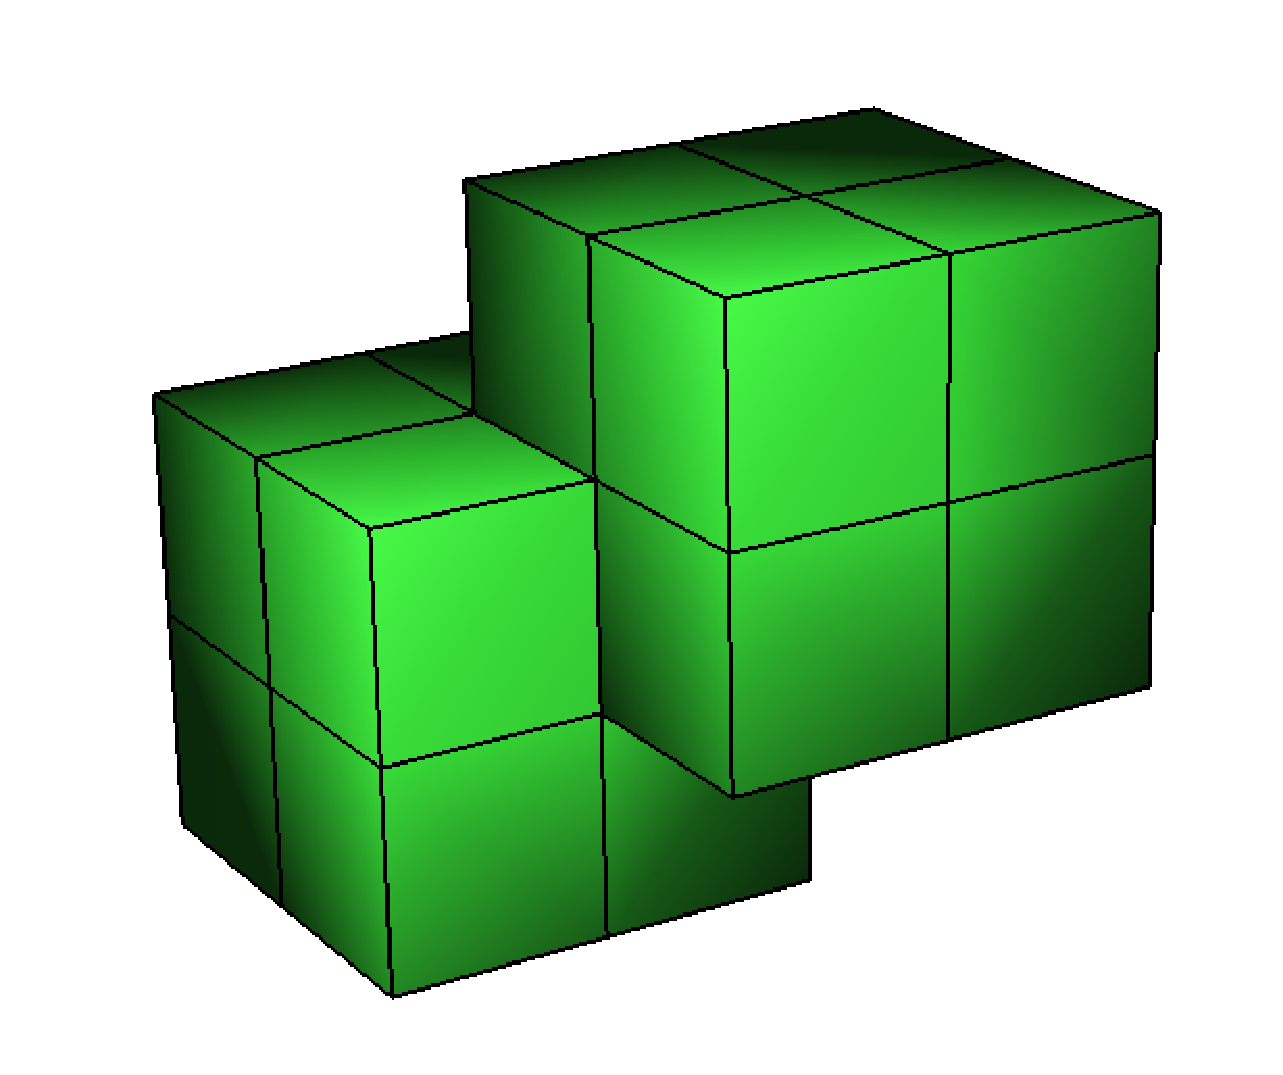
\includegraphics[width=1.6in]{images/twocubes_mesh.eps} &
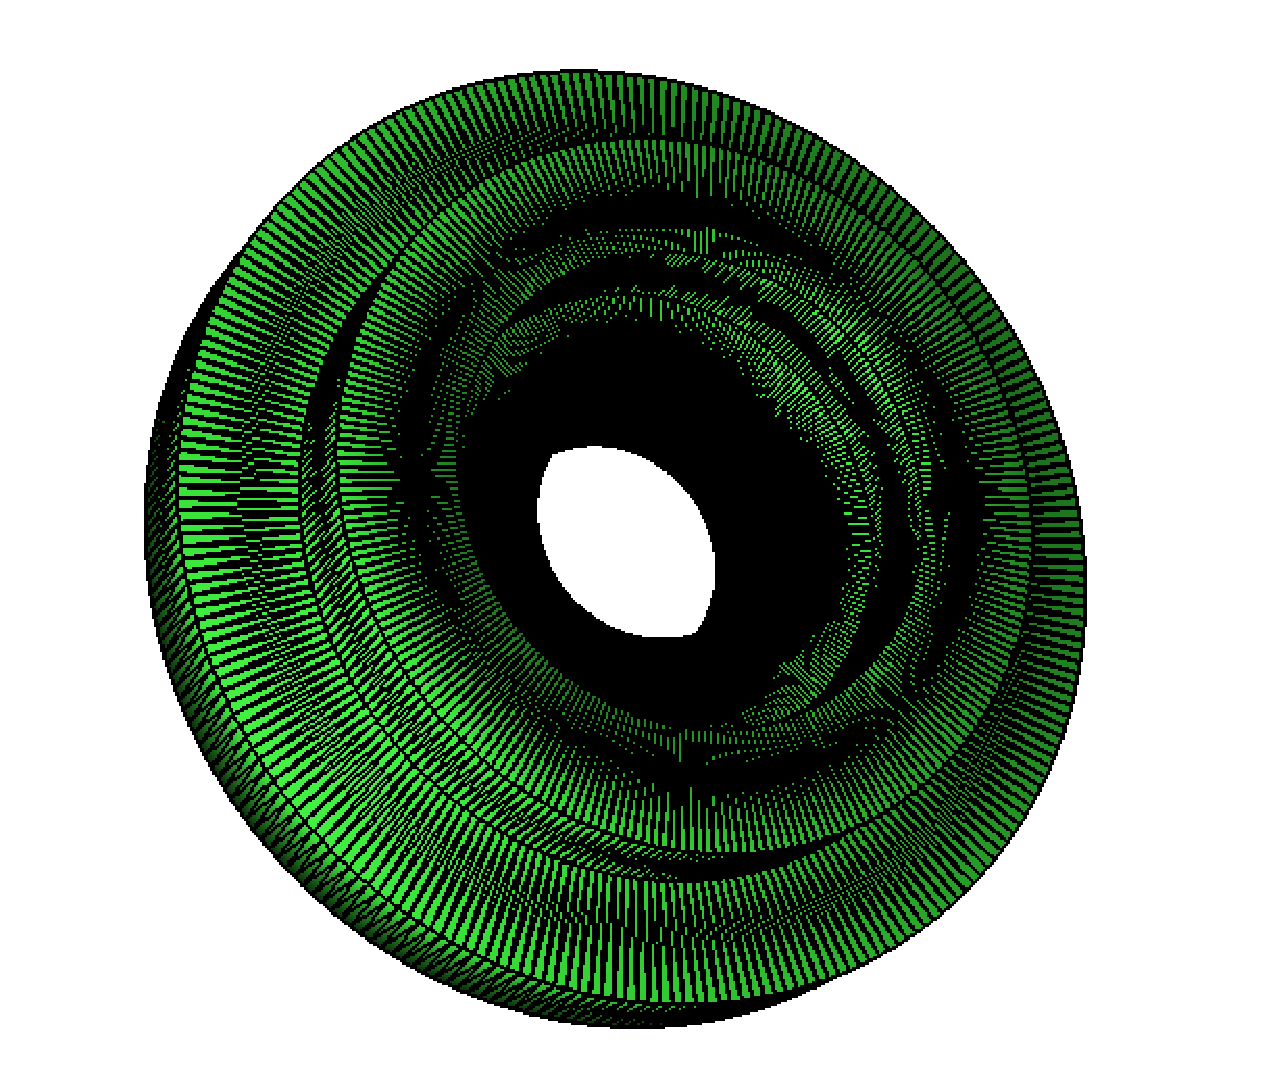
\includegraphics[width=1.6in]{images/flange_mesh.eps} &
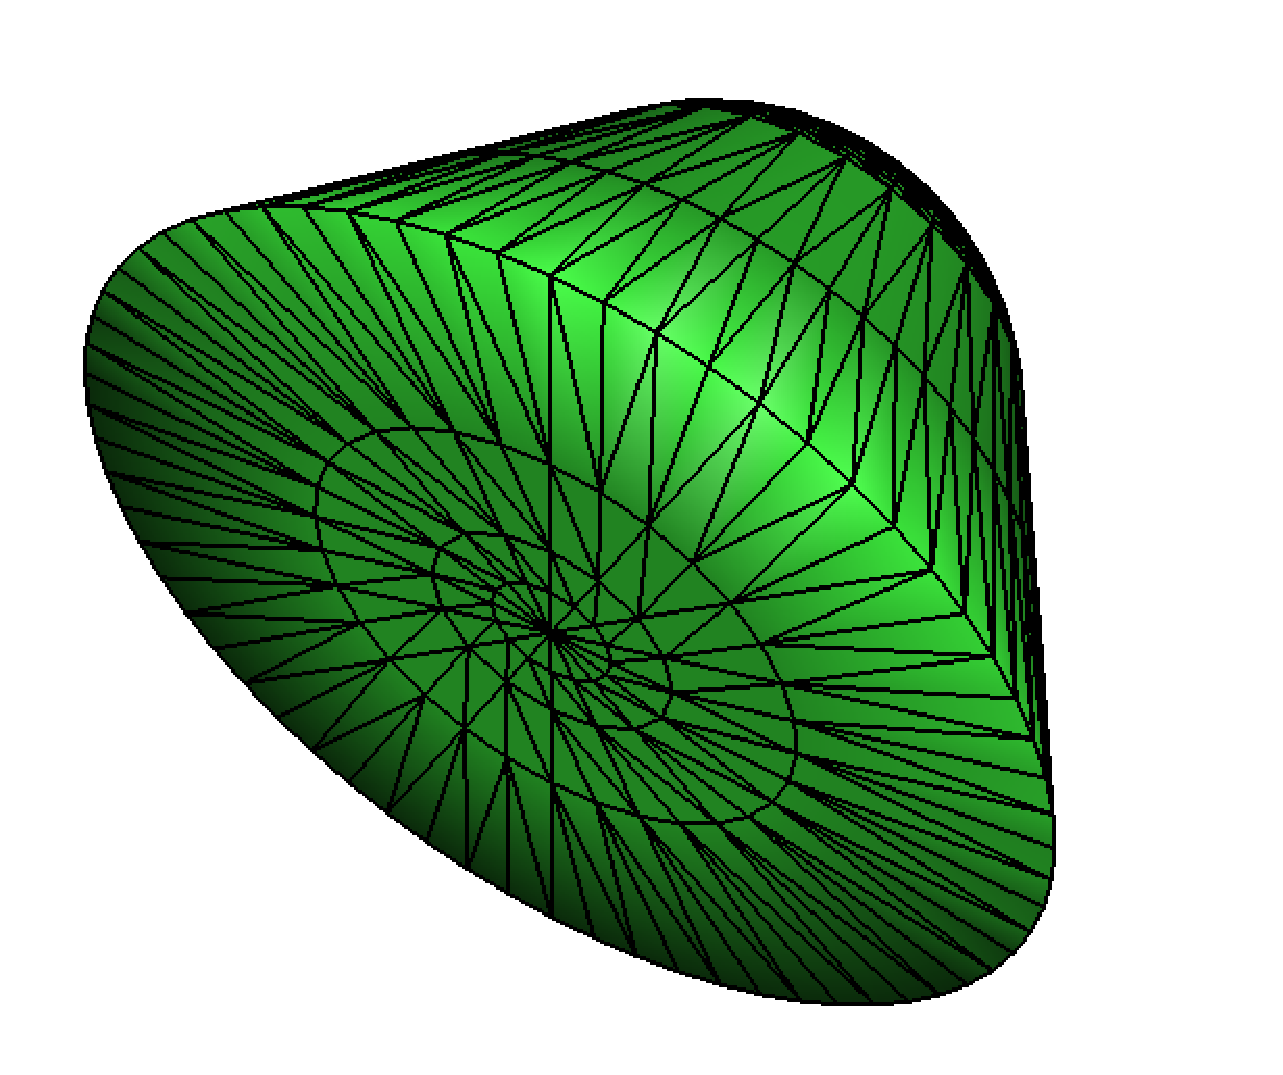
\includegraphics[width=1.6in]{images/smooth_tip_cone_mesh.eps} &
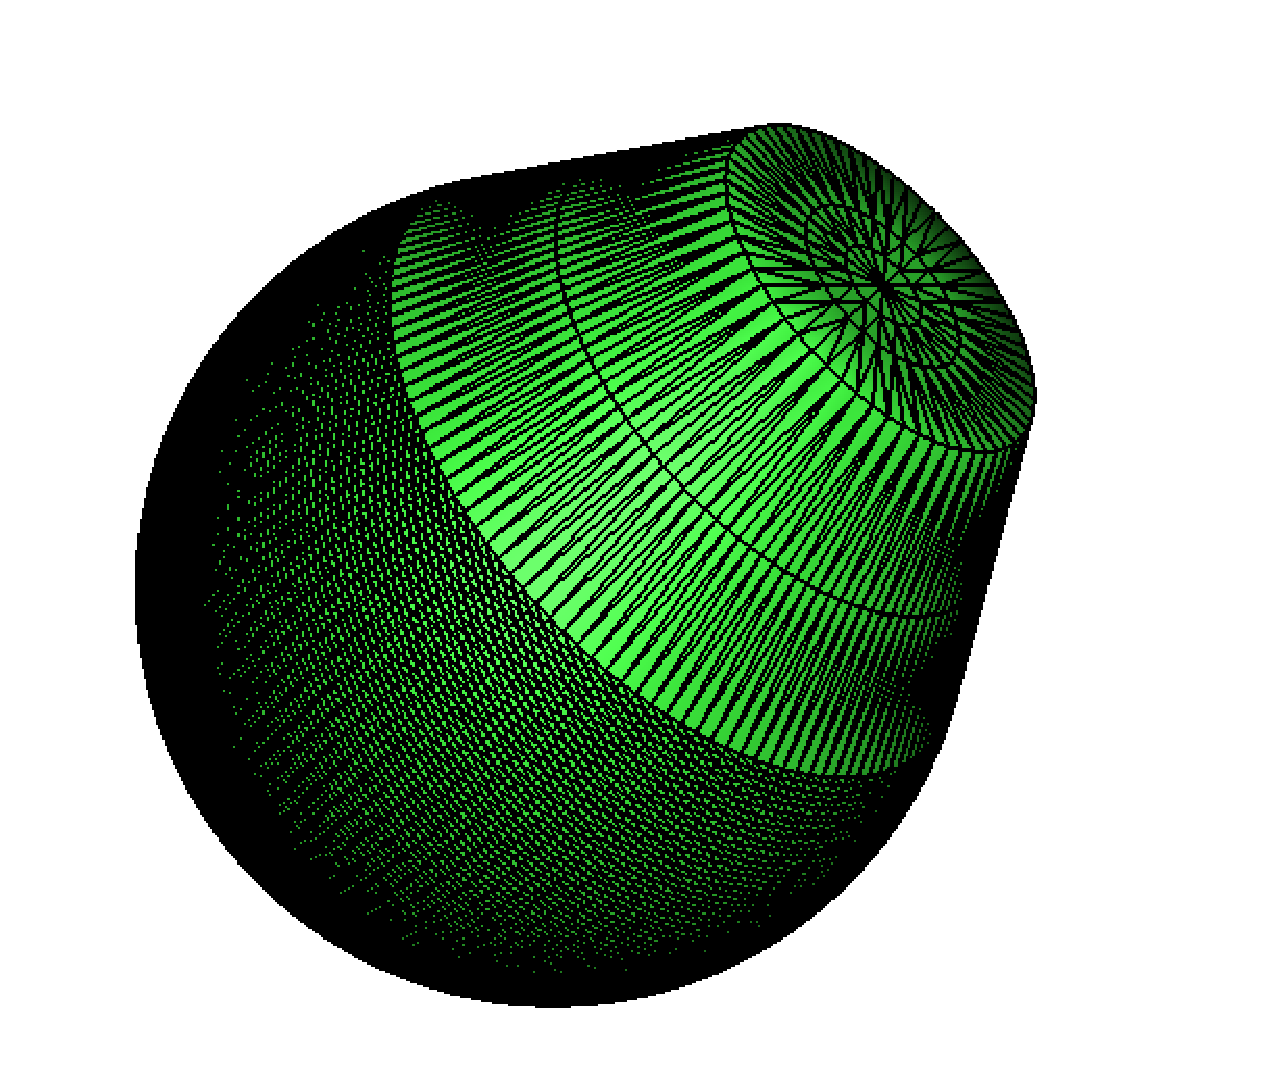
\includegraphics[width=1.6in]{images/cannon_mesh.eps}
\\
(a) TwoCubes & (b) Flange & (c) Smooth Tip Cone & (d) Cannon \\
\end{tabular}
\caption{Polygonal meshes representing level sets.}
\label{fig:mesh}
\end{figure*}

\section{Experimental Results on Synthetic Data}\label{sec:synData}
\label{section:results}

\subsection{Synthetic Scalar and Gradient Data}
\label{section:synthetic}

To measure the quality of our reconstruction,
we used a number of synthetic scalar and gradient datasets.
(See Figure~\ref{fig:synthetic_data}.)
Given a point $p$,
let $f^{L_1}_{p}(q)$ be the $L_1$ distance from $p$ to $q$.
A {\em Cube} dataset is generated by sampling $f^{L_1}_p$
and its gradients on vertices of the regular grid.

Level sets of $f^{L_1}_p$ are cubes whose edges are
parallel to the coordinate axes
and whose facets are orthogonal to those axes.
By rotating $f^{L_1}_p$ around $p$, 
we can generate a scalar field whose level sets are cubes
that are not axis-aligned.
By taking the minimum of two (rotated) scalar fields, 
$f^{L_1}_p$ and $f^{L_1}_{p'}$, 
centered around two different points, $p$ and $p$', respectively,
we get a scalar field whose level sets are the boundaries
of the unions of the two cubes.
(See Figure~\ref{fig:synthetic_data}(a).)
We call a regular grid sampling of such a scalar field
and its gradients a {\em TwoCubes} dataset.
The isosurface of a TwoCubes dataset has twenty 0-dimensional features,
fourteen of which are cube corners and six of which are ``saddle points''
where the two boundaries of two cubes meet.
We use the TwoCubes datasets with various rotations
as test sets for the reconstruction of 0-dimensional features.

Let $\ell$ be a line.
Let $\fCYL_{\ell}(q)$ be the Euclidean distance from point $q$ to $\ell$.
The level sets of $\fCYL_{\ell}(q)$ are infinite cylinders around $\ell$.
Let $\fCII_{\ell,r}(q)$ equal $|\fCYL_{\ell}(q) - r|$.
The level sets of $\fCII_{\ell,r}(q)$  are pairs of infinite cylinders
at equal distances from the cylinder of radius $r$ around $\ell$.
Let $\fPLII_{p,\ell}(q)$ be the (unsigned) distance from $q$ to the plane
that contains point $p$ and is orthogonal to line $\ell$.
Let $\fANN_{p,\ell,r}(q)$ be the maximum 
of $\fCII_{\ell,r}(q)$ and of $\fPLII_{p,\ell}(q)$.
The level sets are the boundaries of thickened annuli.
(See Figure~\ref{fig:synthetic_data}(b).)

The width of the thickened annuli defined by $\fANN_{p,\ell,r}$
equals their height.
We can adjust change the difference between the width and height
by adding constants to $\fCII_{\ell,r}$ or $\fPLII_{p,\ell}(q)$.
Let $\fANN_{p,\ell,r,c_1,c_2}(q)$ be the maximum 
of $\fCII_{\ell,r}(q)+c_1$ and of $\fPLII_{p,\ell}(q)+c_2$.
If $c_1$ is greater than $c_2$, 
then the height is $c_1-c_2$ units greater than the width.
If $c_2$ is greater than $c_1$, 
then the width is $c_2-c_1$ units greater than the height.

Define $\fFR_{p,\ell,r,c}(q)$ as the minimum
of $\fANN_{p,\ell,r,c,0}(q)$ and $\fANN_{p,\ell,r,0,c}(q)$.
The level sets of $\fFR_{p,\ell,r,c}(q)$ are the boundaries
of the unions of two thickened annuli.
(See Figure~\ref{fig:synthetic_data}(c).)
One annuli has height $c$ units greater than its width
while the other has width $c$ units greater than its height.
A {\em Flange} dataset is a regular grid sampling of $\fFR_{p,\ell,r,c}(q)$
and its gradients.
The Flange dataset has no 0-dimensional features.
We use the Flange datasets as test sets
for the reconstruction of 1-dimensional features.

We use two other types of datasets to test our algorithm on dihedral
angles other than $90^\circ$.
A cone is defined by an apex $p$, an axis direction $\zeta$,
and an angle $\alpha < 90^\circ$.
The cone is the union of all the rays from $p$ forming angle $\alpha$
with $\zeta$.
Let $\ell$ be the directed line through $p$ with direction $\zeta$,
i.e. the cone axis.
Let $\pi_{\ell}(q)$ be the projection of point $q$ on $\ell$.
Let $D_1(q)$ be the distance from $p$ to $\pi_{\ell}(q)$
and let $D_2(q)$ be the signed distance from $\pi_{\ell}(q)$ to $p$.
(The distance is negative if $\pi_\ell(q)-p$ points in the opposite
direction from $\zeta$.)
Define $\fCN_{p,\zeta,\alpha}(q)$ 
as $\cos(\alpha) D_1(q) - \sin(\alpha) D_2(q)$.
Function $\fCN_{p,\zeta,\alpha}(q)$ is the signed distance
from point $q$ to its orthogonal projection on the cone,
when that orthogonal projection exists.
The level sets of $\fCN_{p,\zeta,\alpha}(q)$ are cones
with axis $\ell$.

We truncate the cone by defining a plane orthogonal to $\ell$.
Let $p'$ be a point on ray $p+t\zeta$
where $\zeta$ is a unit vector.
Let $\fPL_{p',\zeta}(q)$ equal $(q-p') \cdot \zeta$,
the (unsigned) distance from $q$ 
to the plane containing $p'$ orthogonal to $\zeta$.
Define
\begin{equation*}
\fFR_{p,\zeta,\alpha,p'}(q) = 
\max \left ( \fCN_{p,\zeta,\alpha}(q), \fPL_{p',\zeta}(q), \fPL_{p',-\zeta}(q)
\right ) .
\end{equation*}
The level sets of $\fFR_{p,\zeta,\alpha,p'}(q)$ are frustra.
(See Figure~\ref{fig:synthetic_data}(d).)

The level sets of $\fFR_{p,\zeta,\alpha,p'}(q)$
have two closed curves forming 1-dimensional features.
The dihedral angle on one of these curves is $90^\circ + \alpha$
while the dihedral angle on the other is $90^\circ - \alpha$.
To generate a field with dihedral angles of $90^\circ + \alpha$
or $90^\circ - \alpha$, but not both,
we modify $\fFR_{p,\zeta,\alpha,p'}(q)$ so that the level sets
are capped by spheres at one end.

Define
\begin{align*}
\fSCN_{p,\zeta,\alpha,p'}(q) & =
\left \{
\begin{array}{ll}
|q-p'| & \mbox{ if } \angle(q,p',p) \le 90^\circ - \alpha,\\
\fCN_{p,\zeta,\alpha}(q) & \mbox{ if } 
  \angle(q,p',p) > 90^\circ - \alpha,
\end{array}
\right .
\\
\fTCN_{p,\zeta,\alpha}(q) & = 
\max \left ( \fSCN_{p,\zeta,\alpha,p'}(q), \fPL_{p',\zeta} \right ).
\end{align*}

A level set of $\fSCN_{p,\zeta,\alpha,p'}(q)$ is a cone
with its tip smoothed.
A level set of $\fSCN_{p,\zeta,\alpha,p'}(q)$ is a truncated cone
with its tip smoothed.
The level set has a single closed curve forming a 1-dimensional feature
with dihedral angle $90^\circ - \alpha$.
The {\em Smooth Tip Cone} dataset is a regular sampling
of $\fTCN_{p,\zeta,\alpha,p'}(q)$ and its gradients.
We use Smooth Tip Cone datasets to evaluate reconstruction
of dihedral angles less than $90^\circ$.

Let $p'$ and $p''$ be points on the ray $p + t \zeta$ where
$|p-p'|$ is less than $(1-\sin(\alpha)) |p-p''|$.
Define
\begin{align*}
\fX_{p,\zeta,\alpha,p''}(q) & =
\left \{
\begin{array}{ll}
|q-p''| & \mbox{ if } \angle(q,p',p) > 90^\circ - \alpha,\\
\fCN_{p,\zeta,\alpha}(q) & \mbox{ if } \angle(q,p',p) \le 90^\circ - \alpha.
\end{array}
\right .
\\
\fCAN_{p,\zeta,\alpha,p',p''}(q) & =
\max \left ( \fX_{p,\zeta,\alpha,p''}(q), \fPL_{p',-\zeta} \right ) .
\end{align*}

A level set of $\fCAN_{p,\zeta,\alpha,p'}(q)$ has the shape of a cannon.
The level set has a single closed curve forming a 1-dimensional feature
with dihedral angle $90^\circ + \alpha$.
The {\em Cannon} dataset is a regular sampling
of $\fCAN_{p,\zeta,\alpha,p'}(q)$ and its gradients.
We use Cannon datasets to evaluate reconstruction
of dihedral angles greater than $90^\circ$.



\begin{table*}[t]
\centering
\begin{tabular}{|l||r|c|c|r|r|r|r|}
\hline
              & \centercol{Num} & & & \centercol{Avg Num} 
                                     & \centercol{Avg Num} 
                                         & \centercol{Avg Num} & \\
Dataset Type & Datasets & Grid Size & Isovalue 
                                 & \centercol{Active Cubes} 
                                    & \centercol{Iso Vert} 
                                        & \centercol{Iso Tri} 
                                             & \centercol{Avg Time} \\
\hline
\hline
TwoCubes & 34 & \gDim{150} & 20.1 & 25K & 22K & 45K & 0.8 sec \\
\hline
Flange & 40 & \gDim{200} & 10.1 & 90K & 75K & 150K & 1.8 sec \\
\hline
Smooth Tip Cone & 15 & \gDim{100} & 10.2 & 4K & 3.5K & 7K & 0.2 sec \\
\hline
Cannon & 15 & \gDim{100} & 0.0 & 7K & 7K & 14K & 0.2 sec \\
\hline
\end{tabular}

\caption{Synthetic test dataset sizes, isovalues, and average statistics
on isosurfaces produced by SHREC.
Average number of active cubes, 
average number of isosurface vertices,
average number of isosurface triangles,
and average SHREC running time.
All isosurface quadrilaterals are triangulated
before counting the number of isosurface triangles.
Because SHREC merges isosurface vertices, the average number of isosurface
vertices is less than the average number of active cubes.
}

\label{table:datasets}

\end{table*}

\subsection{Gradients}

Algorithm SHREC requires gradients at the grid vertices.
Exact formulas can be given for gradients
for each of the scalar fields described in the previous section.
However, if scalar data is acquired from scanning devices such as CT scanners,
only scalar information is available.
In~\cite{bw-crgsd-15},
we describe an algorithm, Religrad, for constructing a set 
of reliable gradients from scalar data.
We evaluated SHREC both on gradients computed by exact formulas
and on the gradients produced by Religrad from the scalar data.

\subsection{Measurements}
\label{section:measure}

For each test scalar field $f$ and test isovalue $\sigma$,
we constructed a polygonal mesh which represented the level set,
$f^{-1}(\sigma)$.
(See Figure~\ref{fig:mesh}.)
The polygonal mesh was designed specifically for each surface
to accurately represent the 0-dimensonal and 1-dimensional features
on the surface.

To compare isosurfaces constructed by different software on different scales,
we rescaled every isosurface and polygonal mesh to lie in the unit cube.
Our isosurfaces were computed from grids 
of $150 \times 150 \times 150$ or $200 \times 200 \times 200$
so this rescaled the cube size to about $0.005$ units.
We computed the angular distance in the extended neighborhood $\epsilon$
as defined in Section~\ref{section:angular_distance}
between each isosurface and the corresponding polygonal mesh.
We set $\epsilon$ equal to $0.01$ or about twice the cube size
for the extended neighborhood.

We also used the degree test as described in~\cite{bw-cisec-13}
to measure errors in reconstructing sharp features.
We extracted the 1-skeleton of isosurface edges with dihedral angle 
less than $140^\circ$ and counted the number of vertices in the 1-skeleton
with degree other than two.
For an isosurface $\Sigma$,
let $\NneqII(\Sigma)$ be the number of vertices in the 1-skeleton
with degree other than two.
Isosurfaces from the Flange, Smooth Tip Cone and Cannon datasets
should have had zero vertices with degrees other than two.
The number of degree errors for these isosurfaces is $\NneqII(\Sigma)$.
Isosurfaces from the TwoCubes datasets should have had exactly
twenty vertices with degrees other than two.
The number of degree errors for these isosurfaces is $|\NneqII(\Sigma)-20|$.

\begin{figure}[tb]
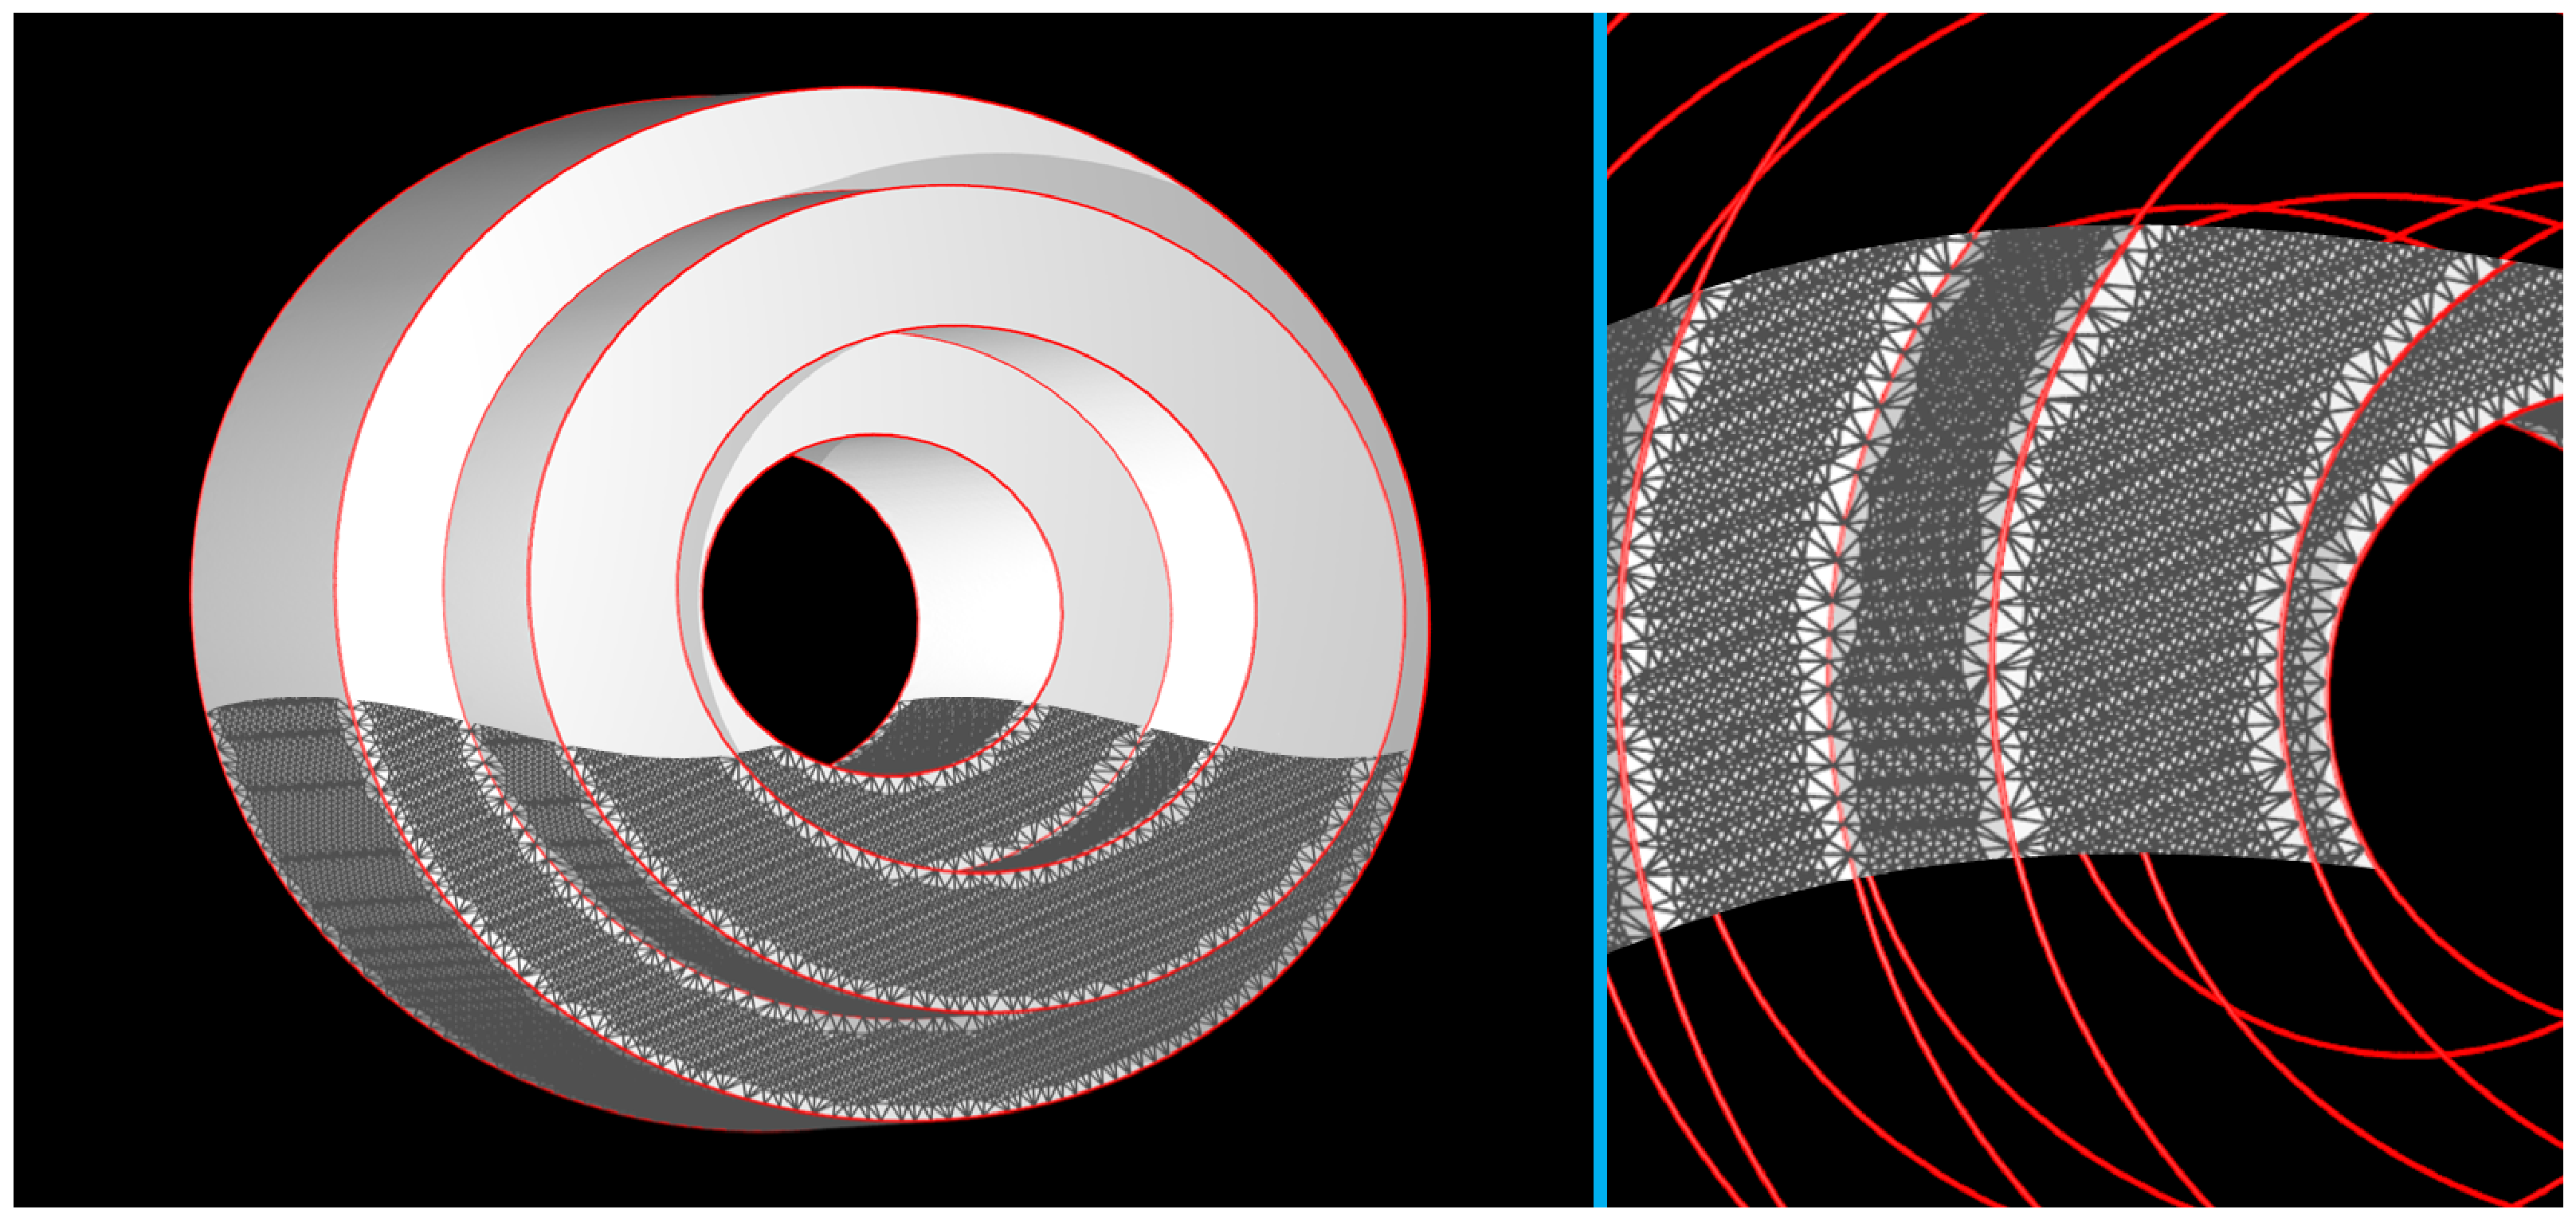
\includegraphics[width=\linewidth]{images/shrecFlangeCombine2.eps}
\caption{SHREC Flange isosurface. ``Sharp" edges (with dihedral angle less than $140^\circ$) are marked in red. 
``Smooth" edges are in dark grey. The magnified region shows a blend of the ``sharp" edges with a subset of the ``smooth" edges.}
\label{fig:flange1}
\end{figure}


\begin{figure*}[tp]
\centering	

%	\subfloat[]{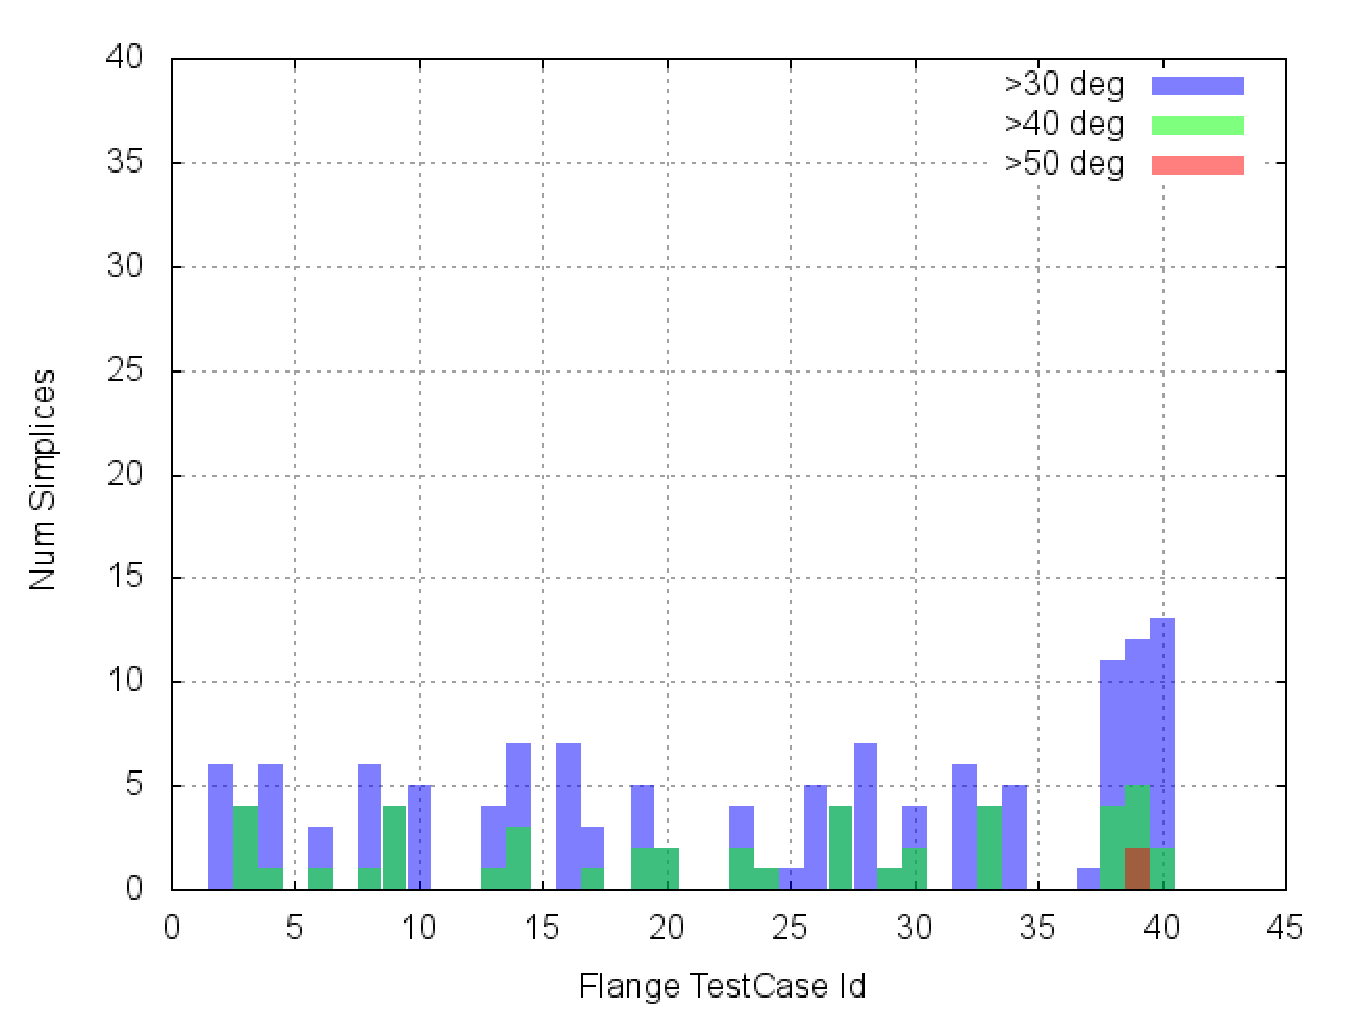
\includegraphics[width=0.33\linewidth]{images/flangeAngle1b.eps}\label{fig:flangeAngle1}}
%	\subfloat[]{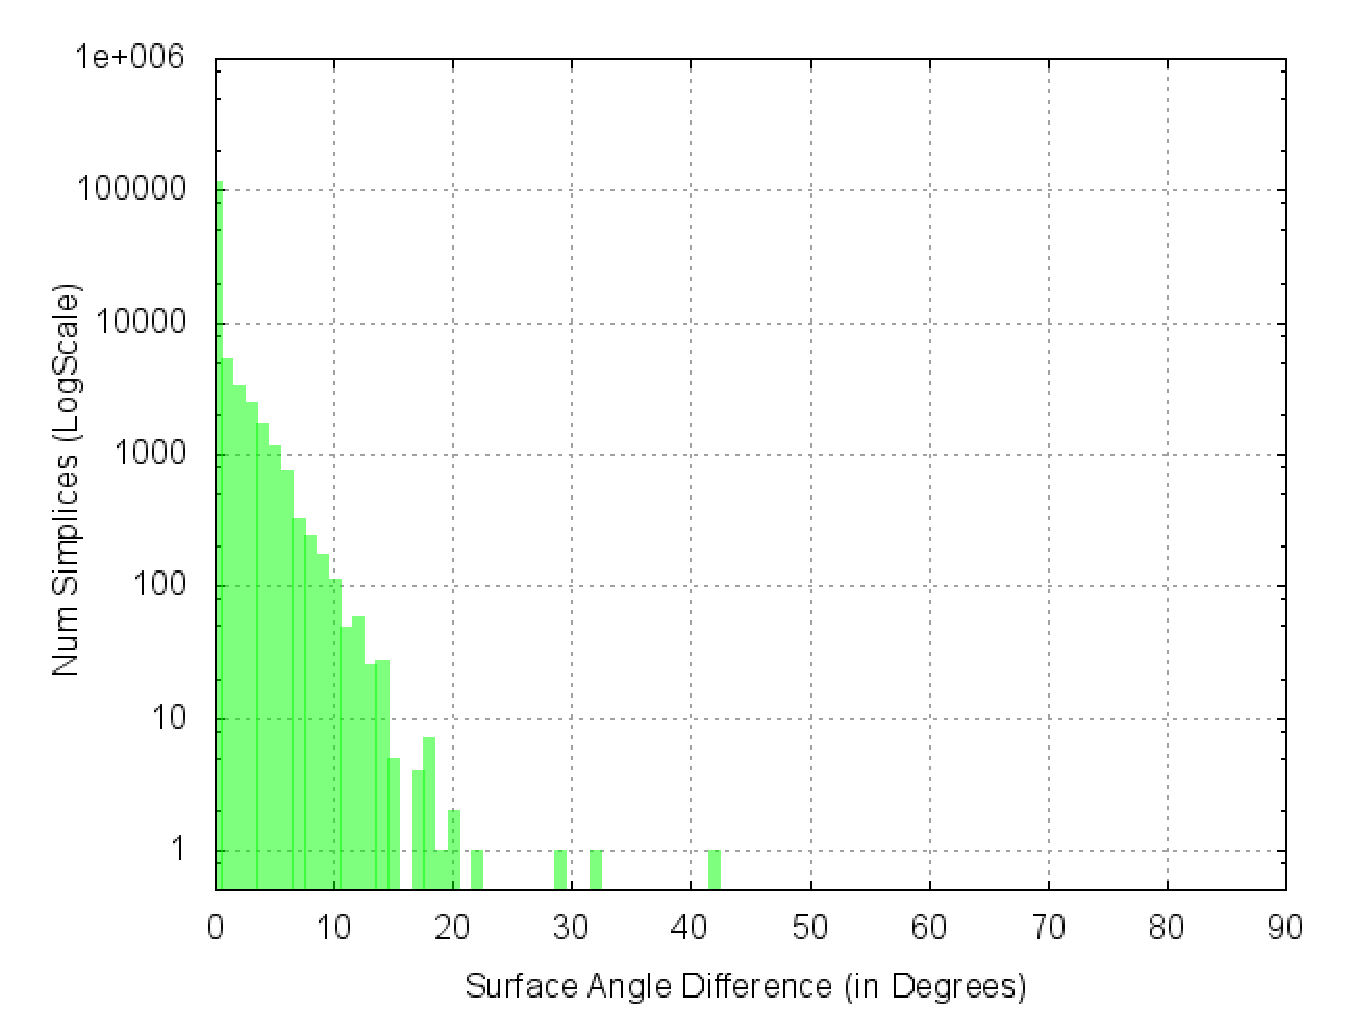
\includegraphics[width=0.33\linewidth]{images/flangeAngle2.eps}\label{fig:flangeAngle2}}
%	\subfloat[]{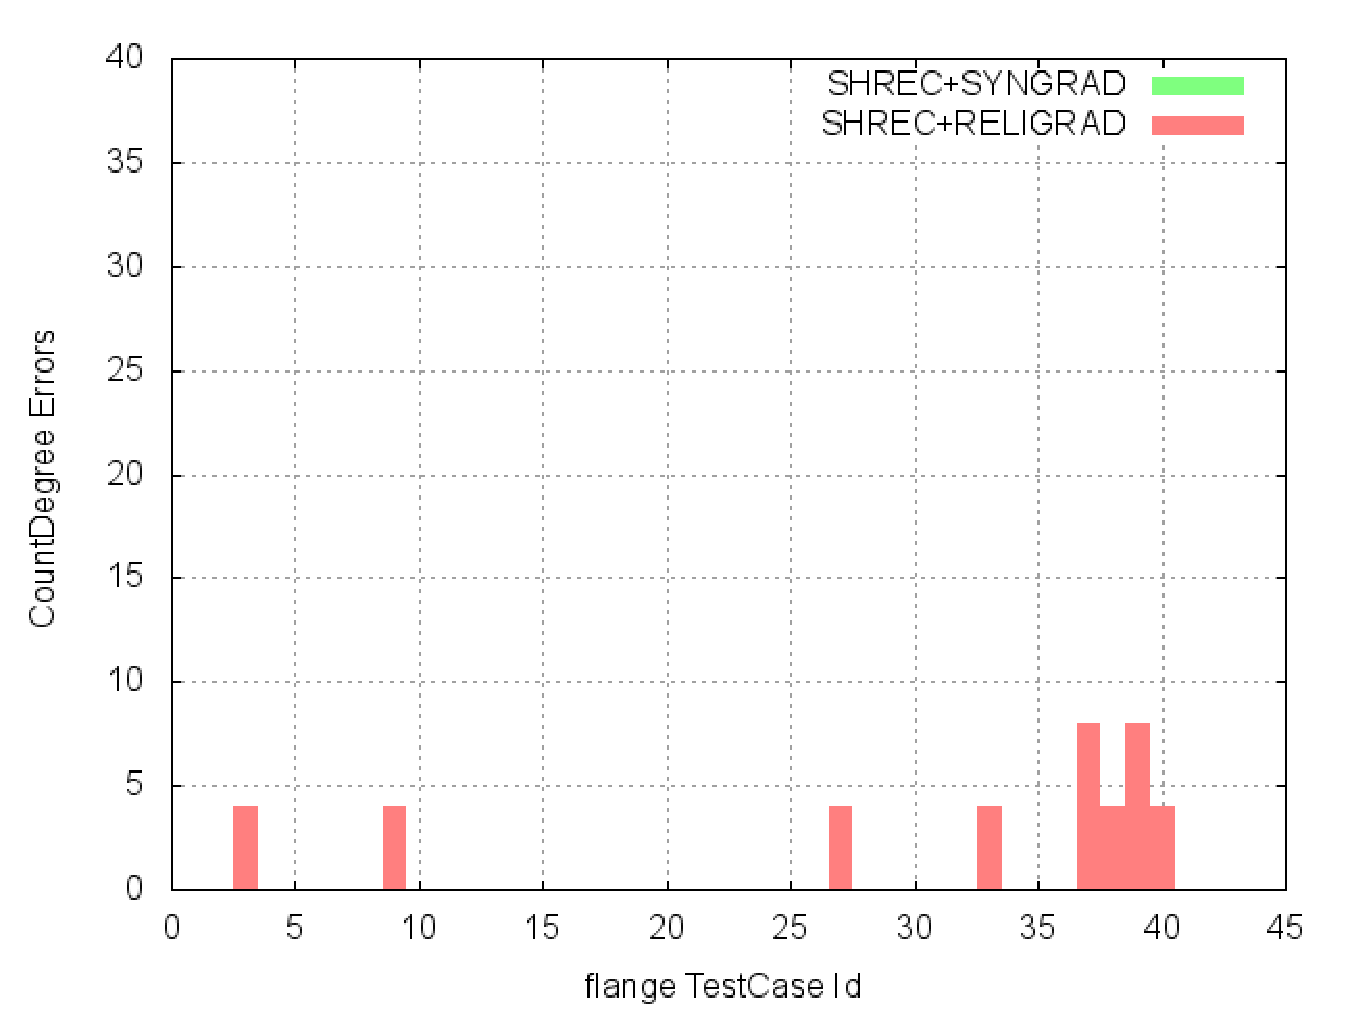
\includegraphics[width=0.33\linewidth]{images/flangeAngle3b.eps}\label{fig:flangeAngle3}}
\subfloat[]{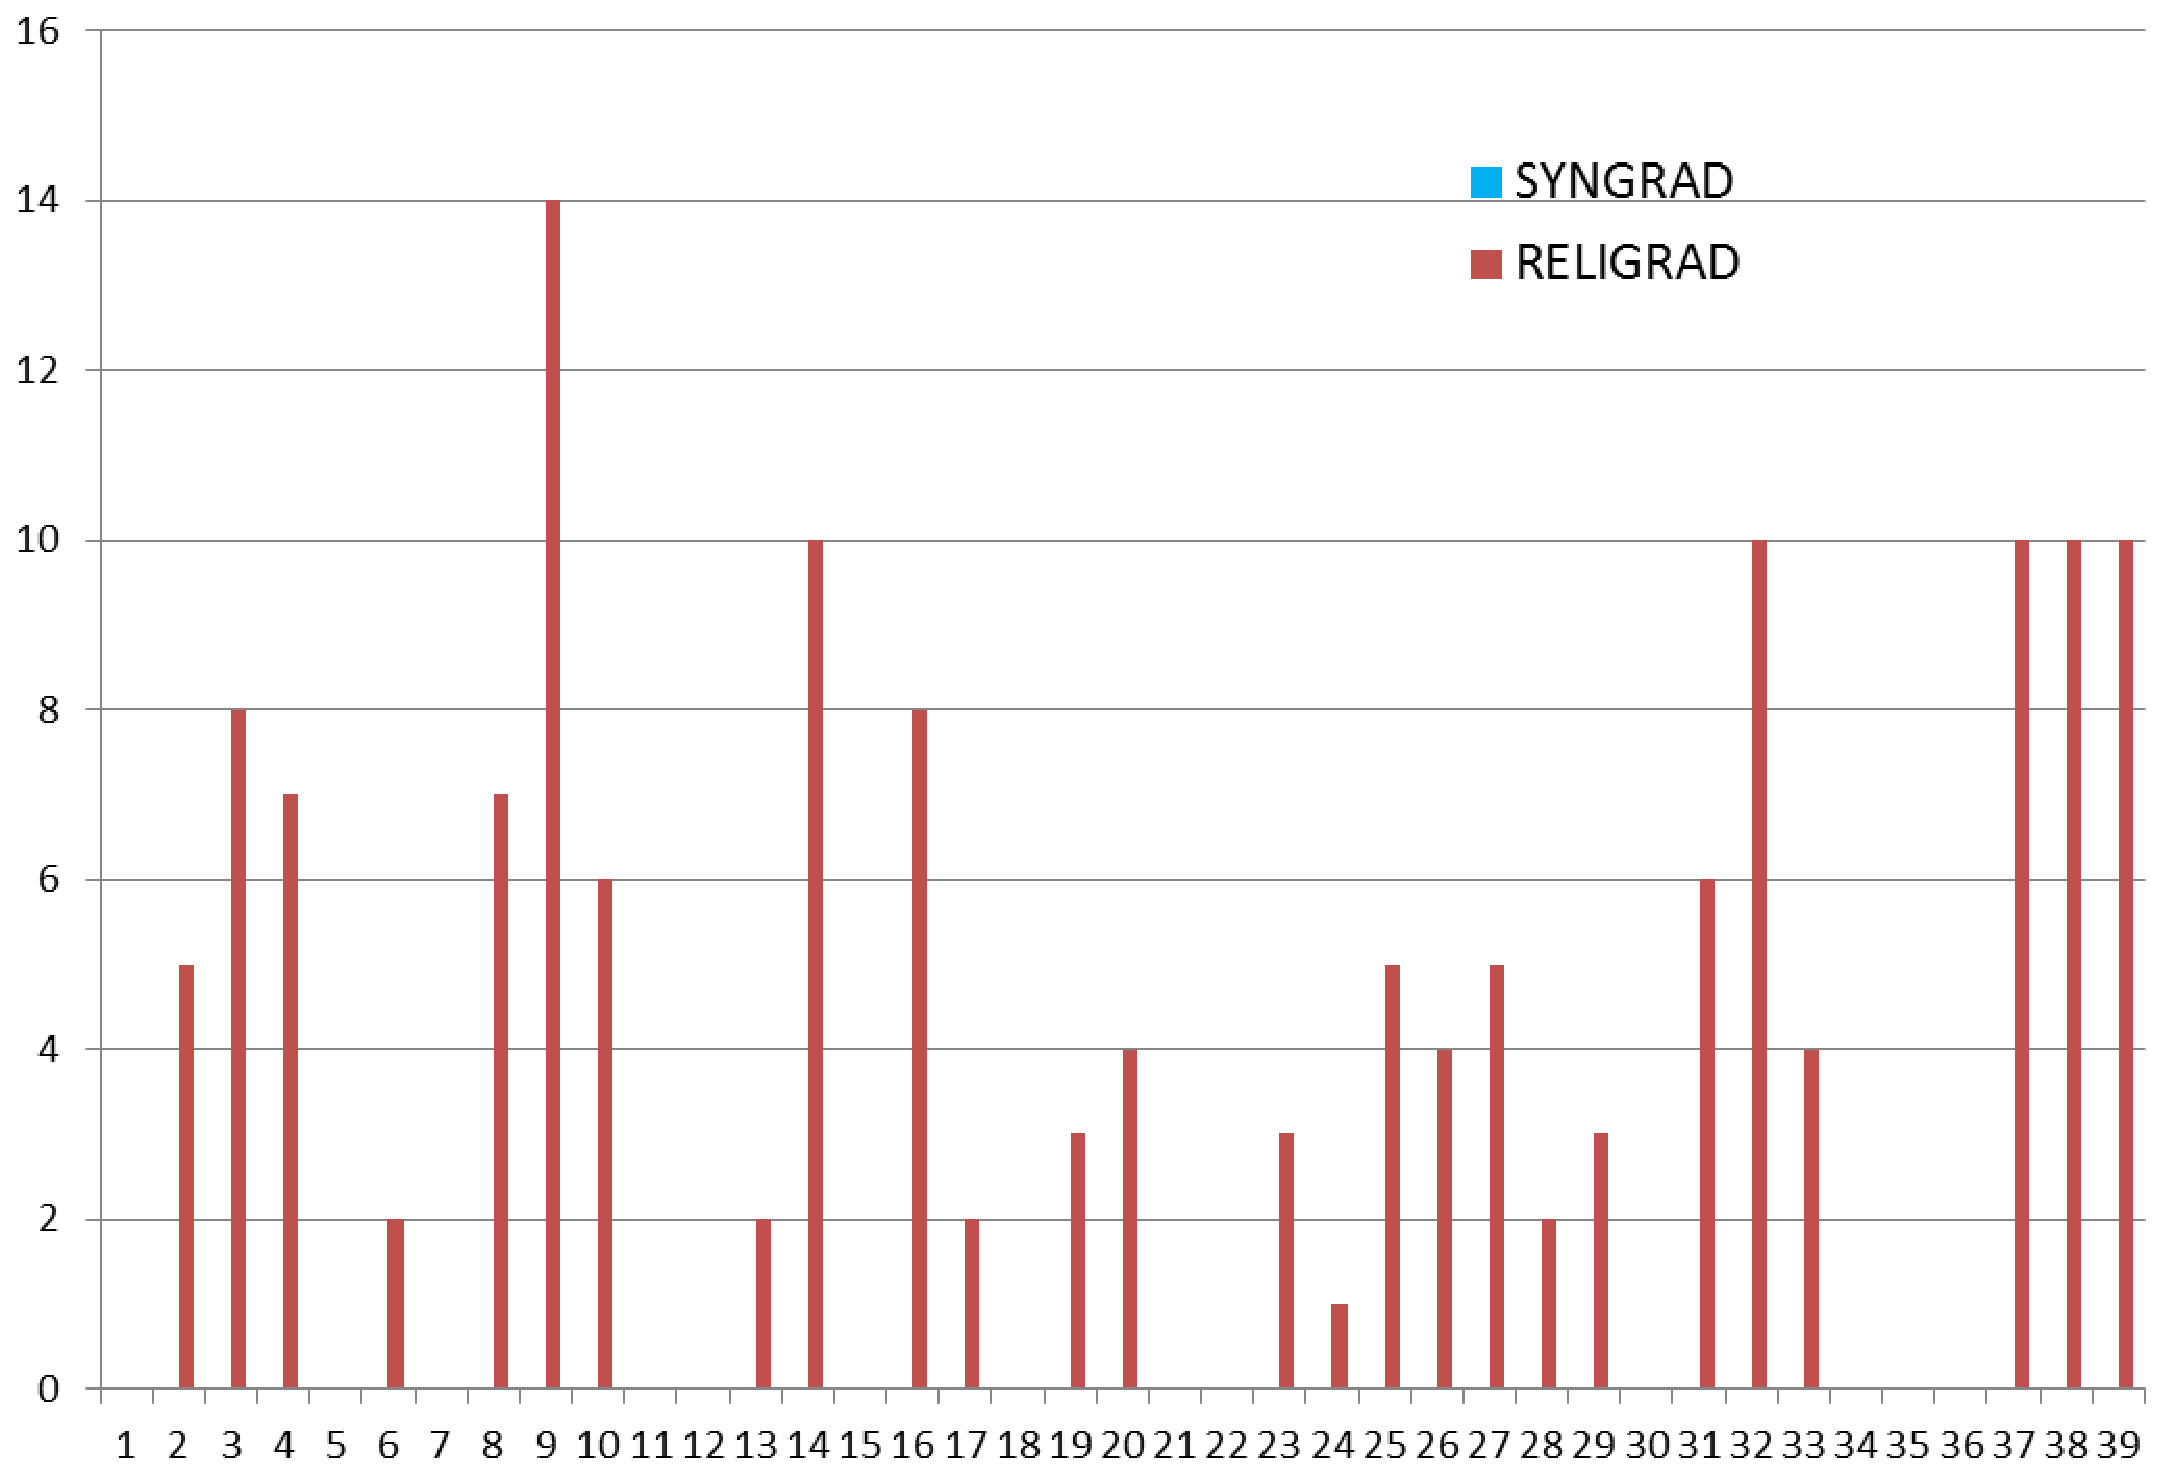
\includegraphics[width=0.3\linewidth]{images/flange_countDegree_shrec.eps}\label{fig:flangeAngle1}}
	\subfloat[]{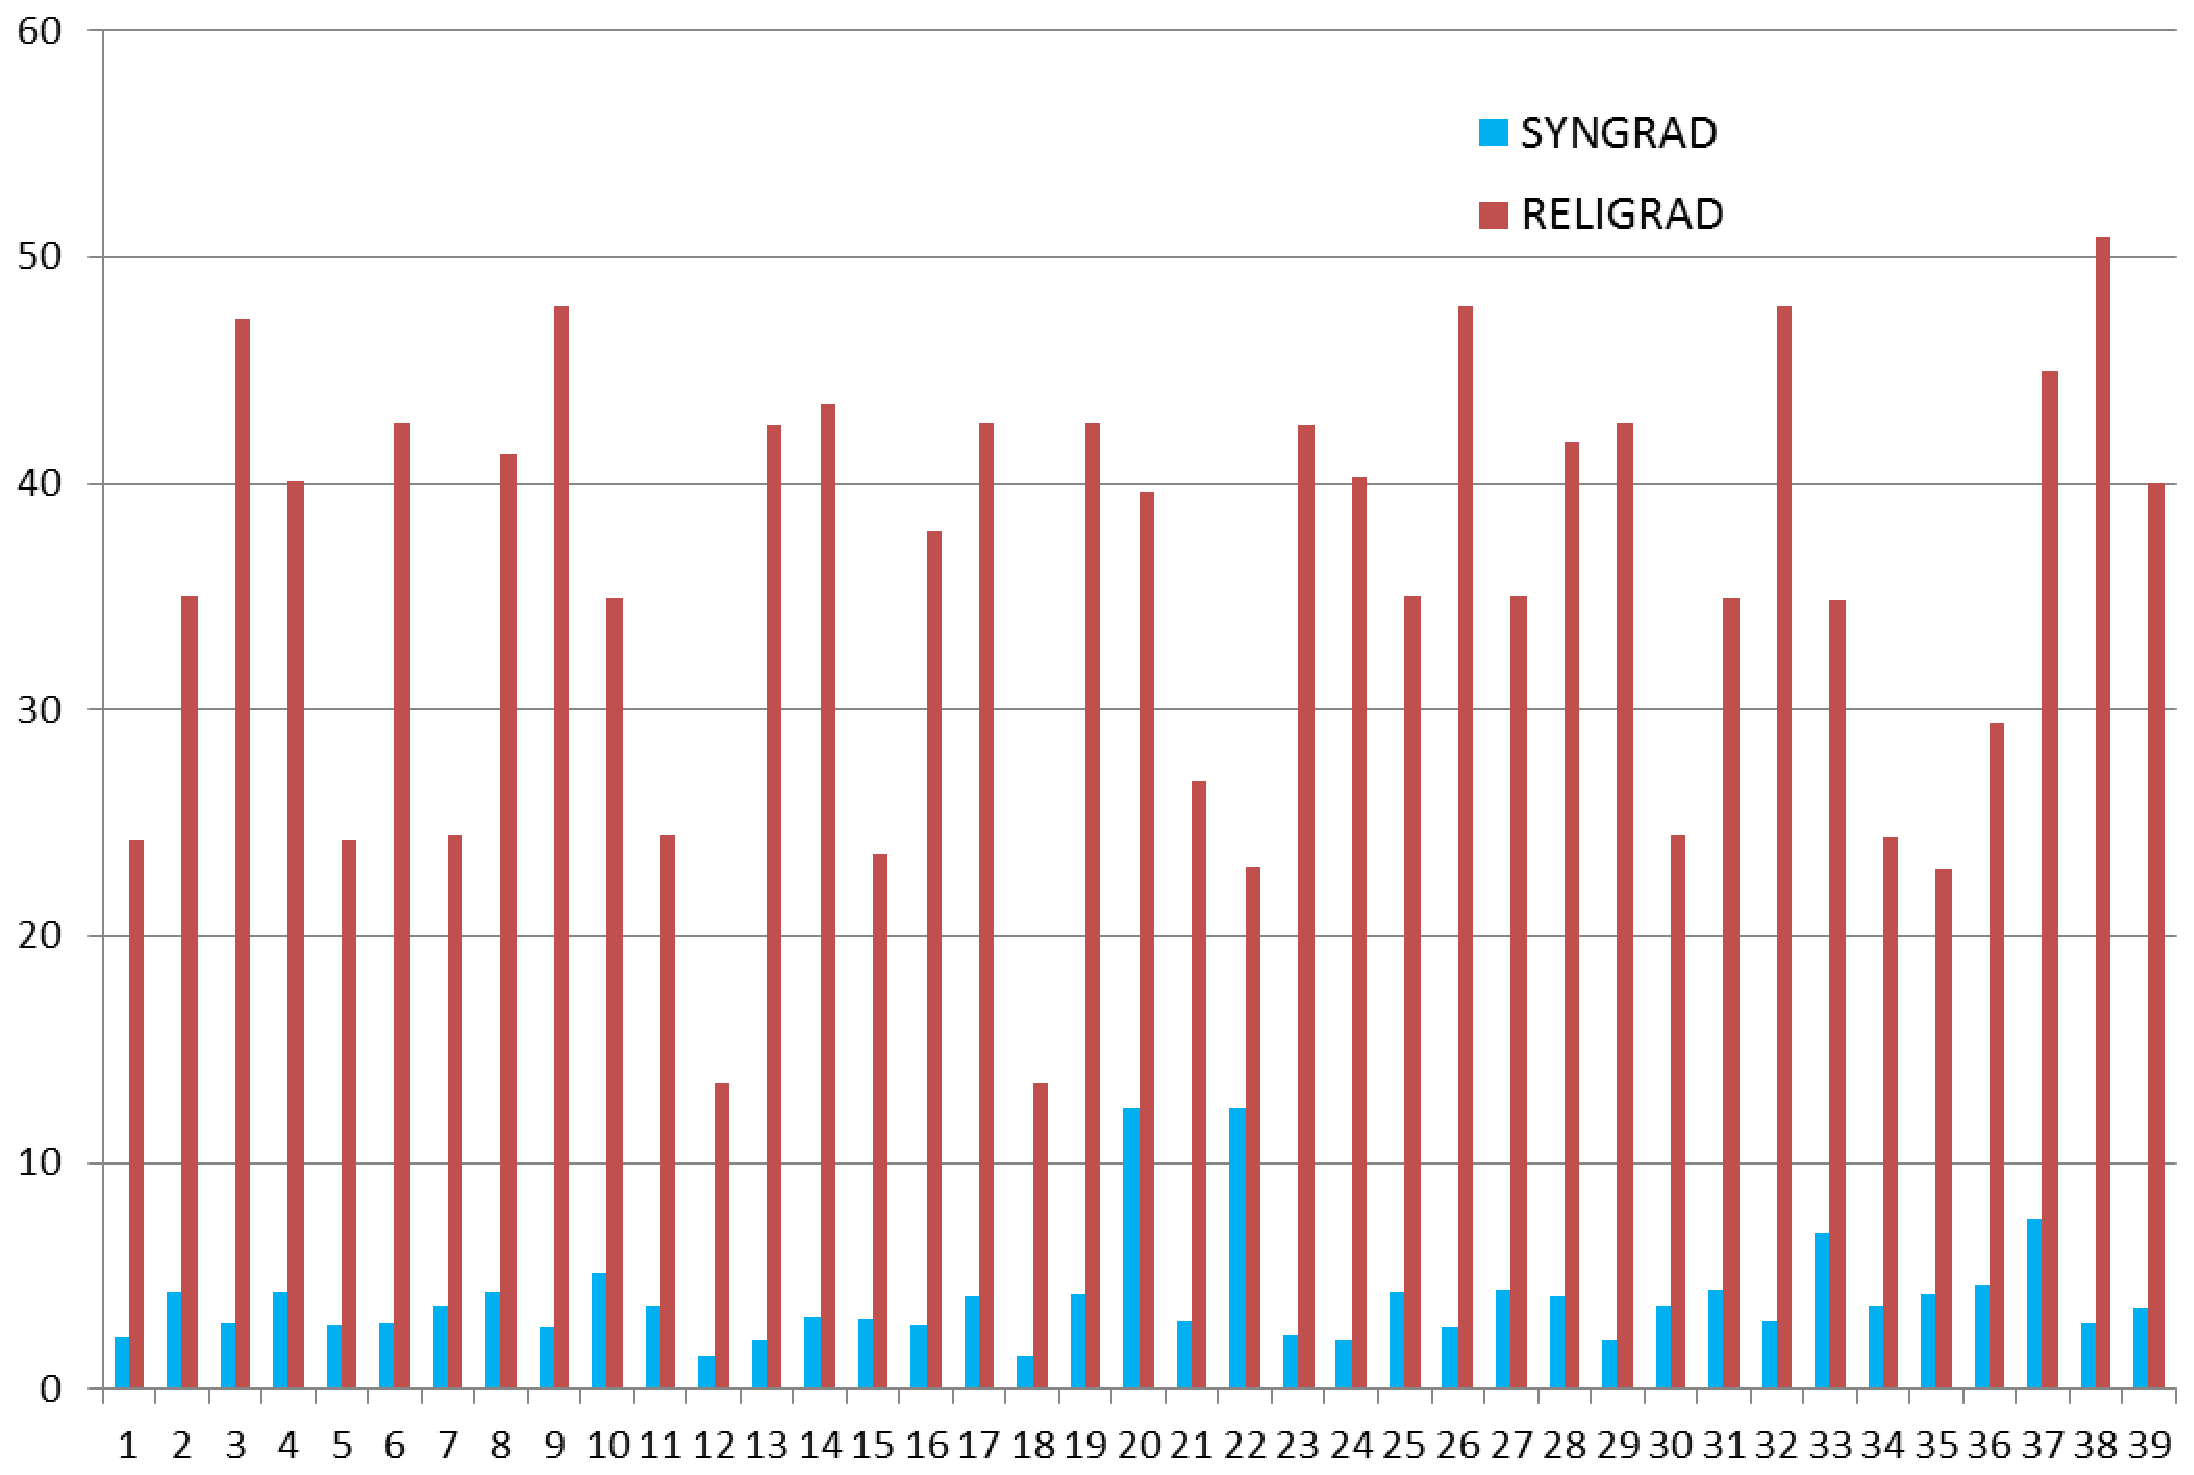
\includegraphics[width=0.3\linewidth]{images/flange_maxAngle_shrec.eps}\label{}}\\
	\subfloat[]{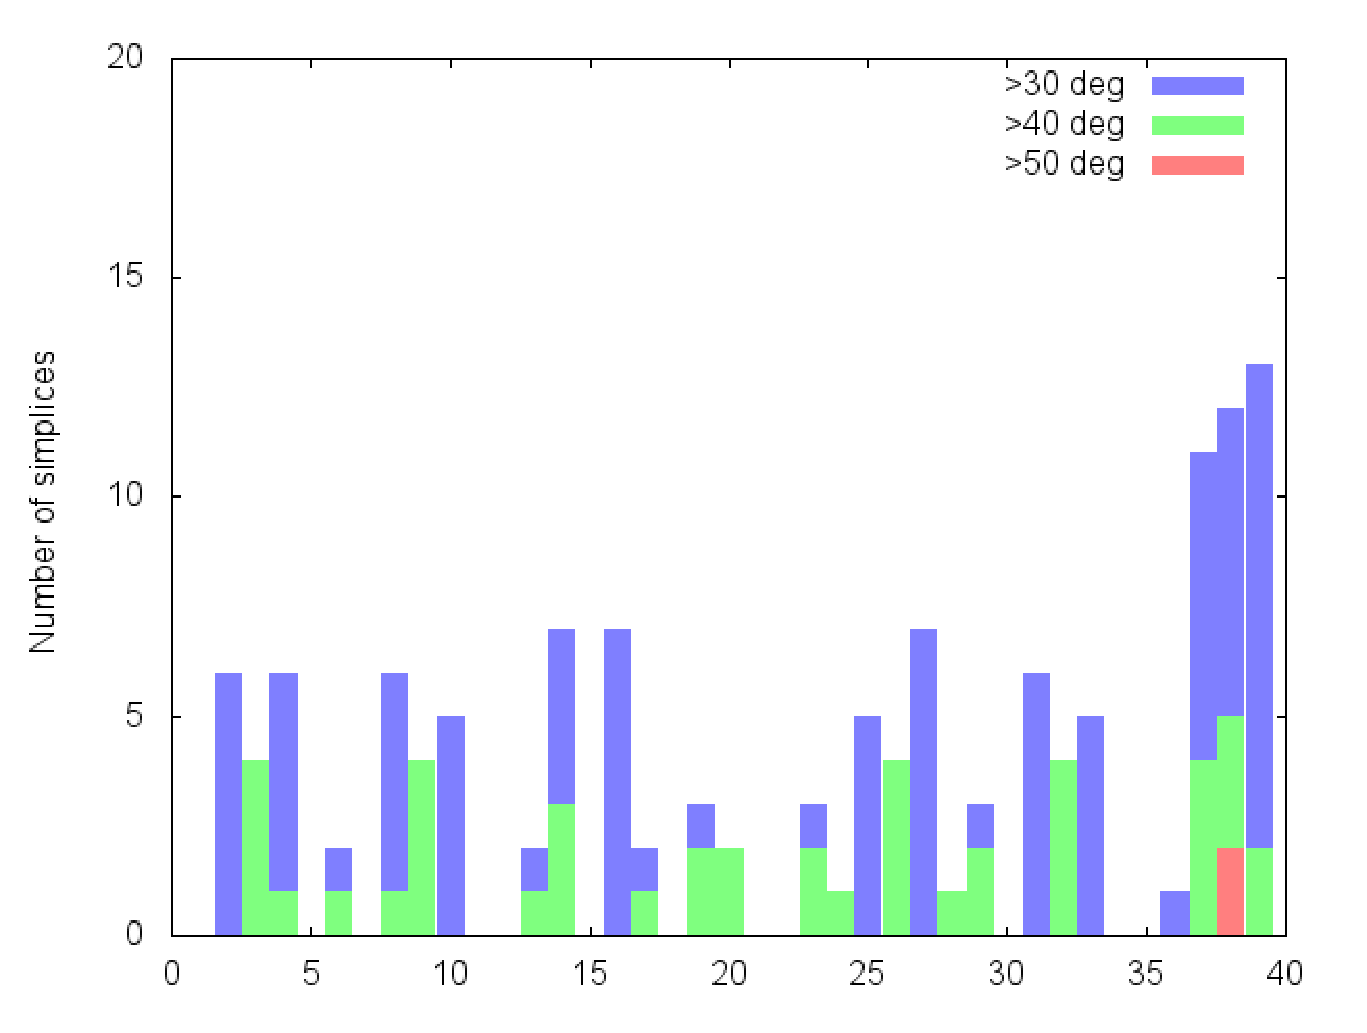
\includegraphics[width=0.3\linewidth]{images/flange_shrec_distribution.eps}\label{}}
\caption{Results of SHREC using exact gradients and Religrad gradients on 39 Flange datasets. 
(a) Number of triangles with angle difference 
to polygonal mesh above 30, 40 and 50 degrees. 
(b) Distribution of triangle normal differences for test case 16.
(Isosurface has approximately $133K$ triangles.)
(c) Number of degree errors in 1-skeleton of sharp edges.
}

\label{fig:flangeAngle}

\vspace{4em}
	\subfloat[]{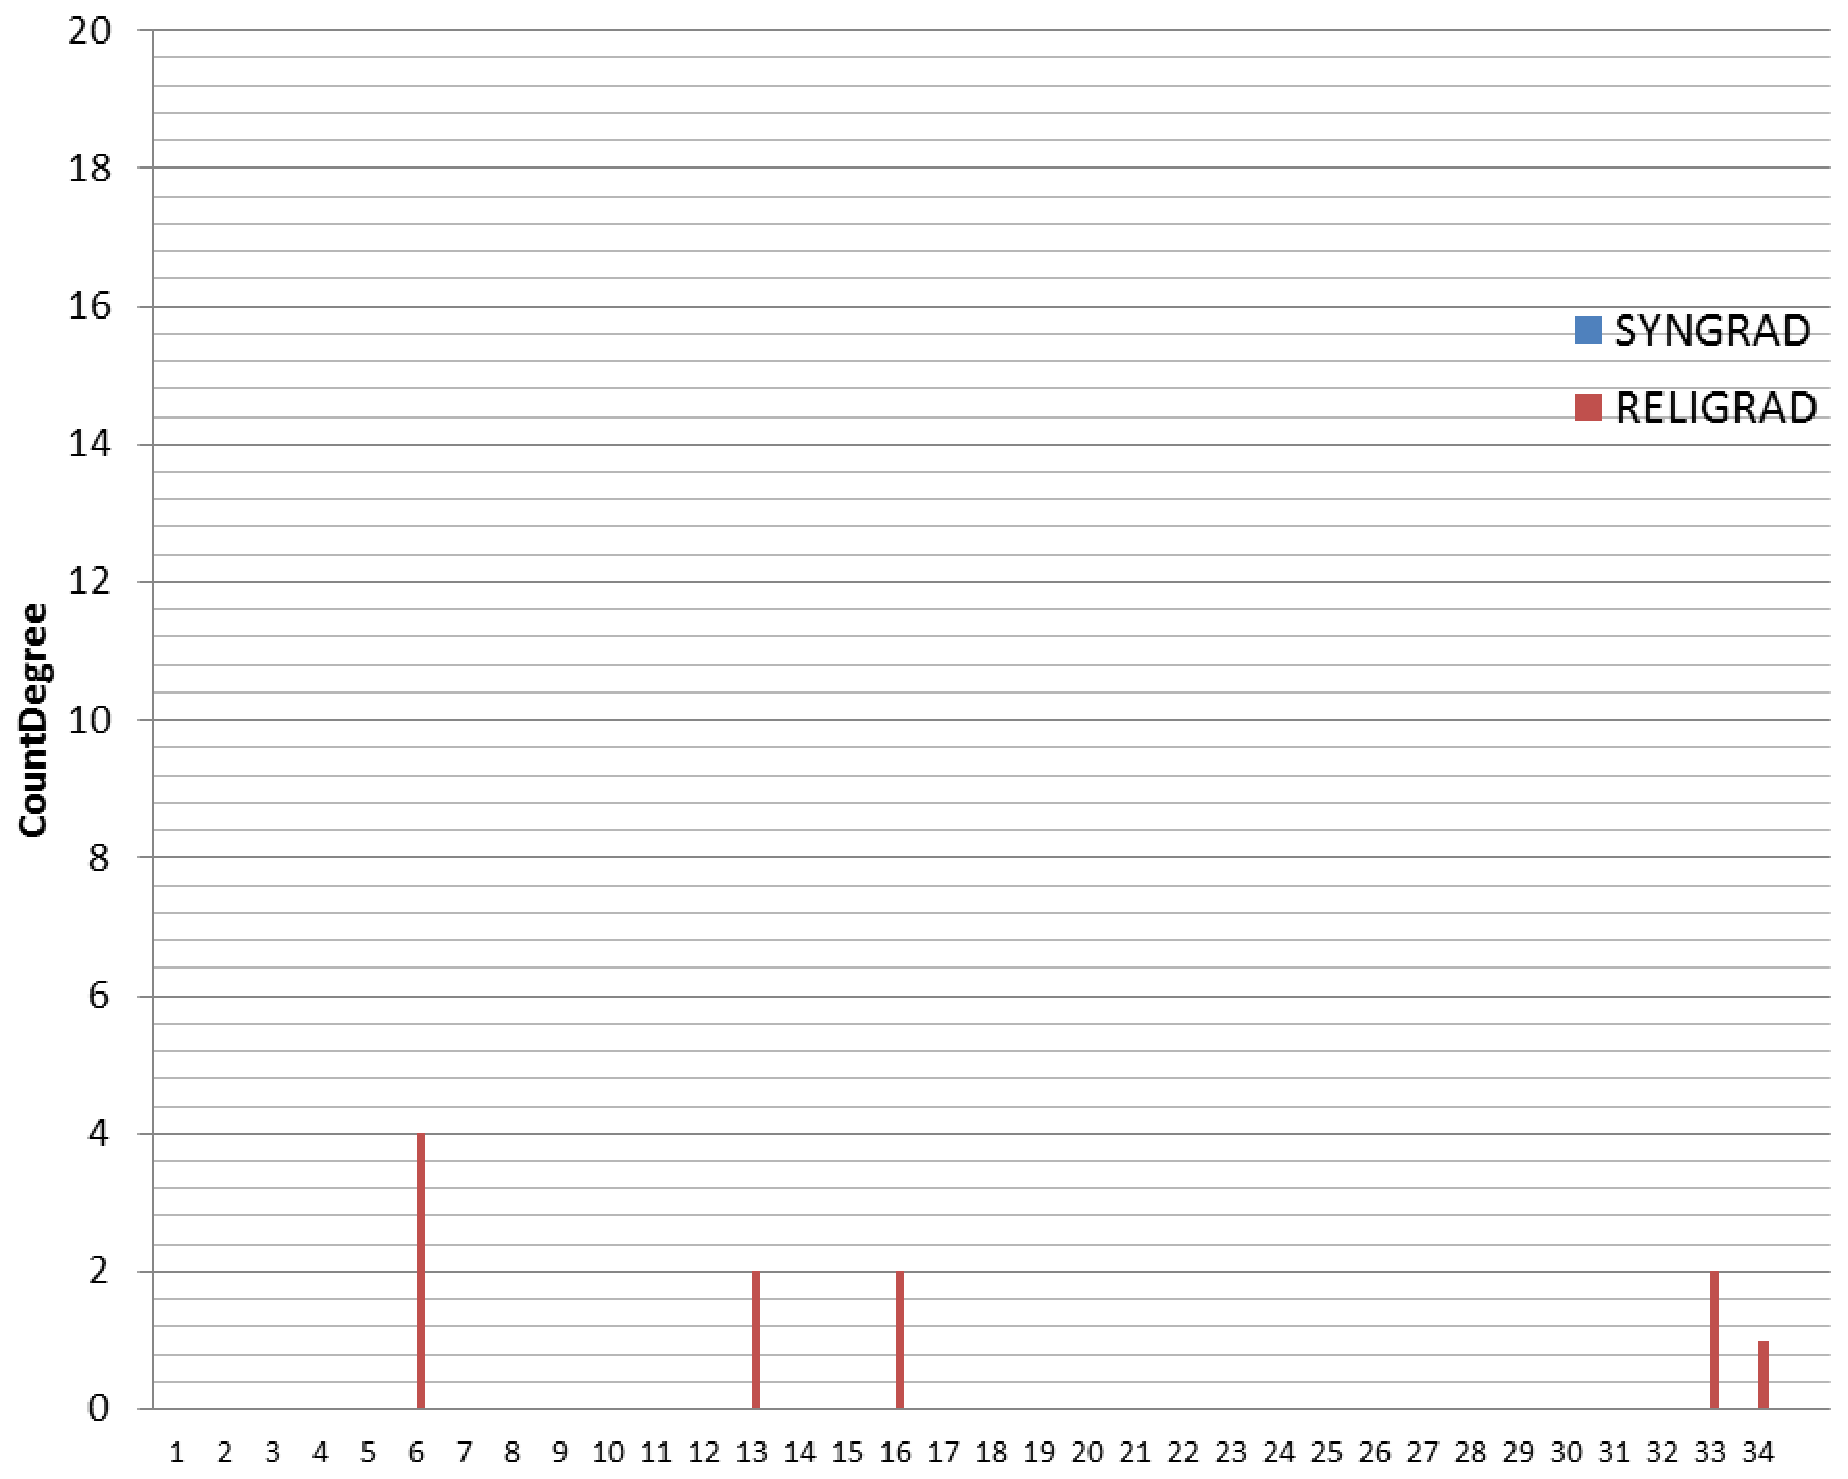
\includegraphics[width=0.3\linewidth]{images/twoCube_countDegree_shrec.eps}\label{}}
	\subfloat[]{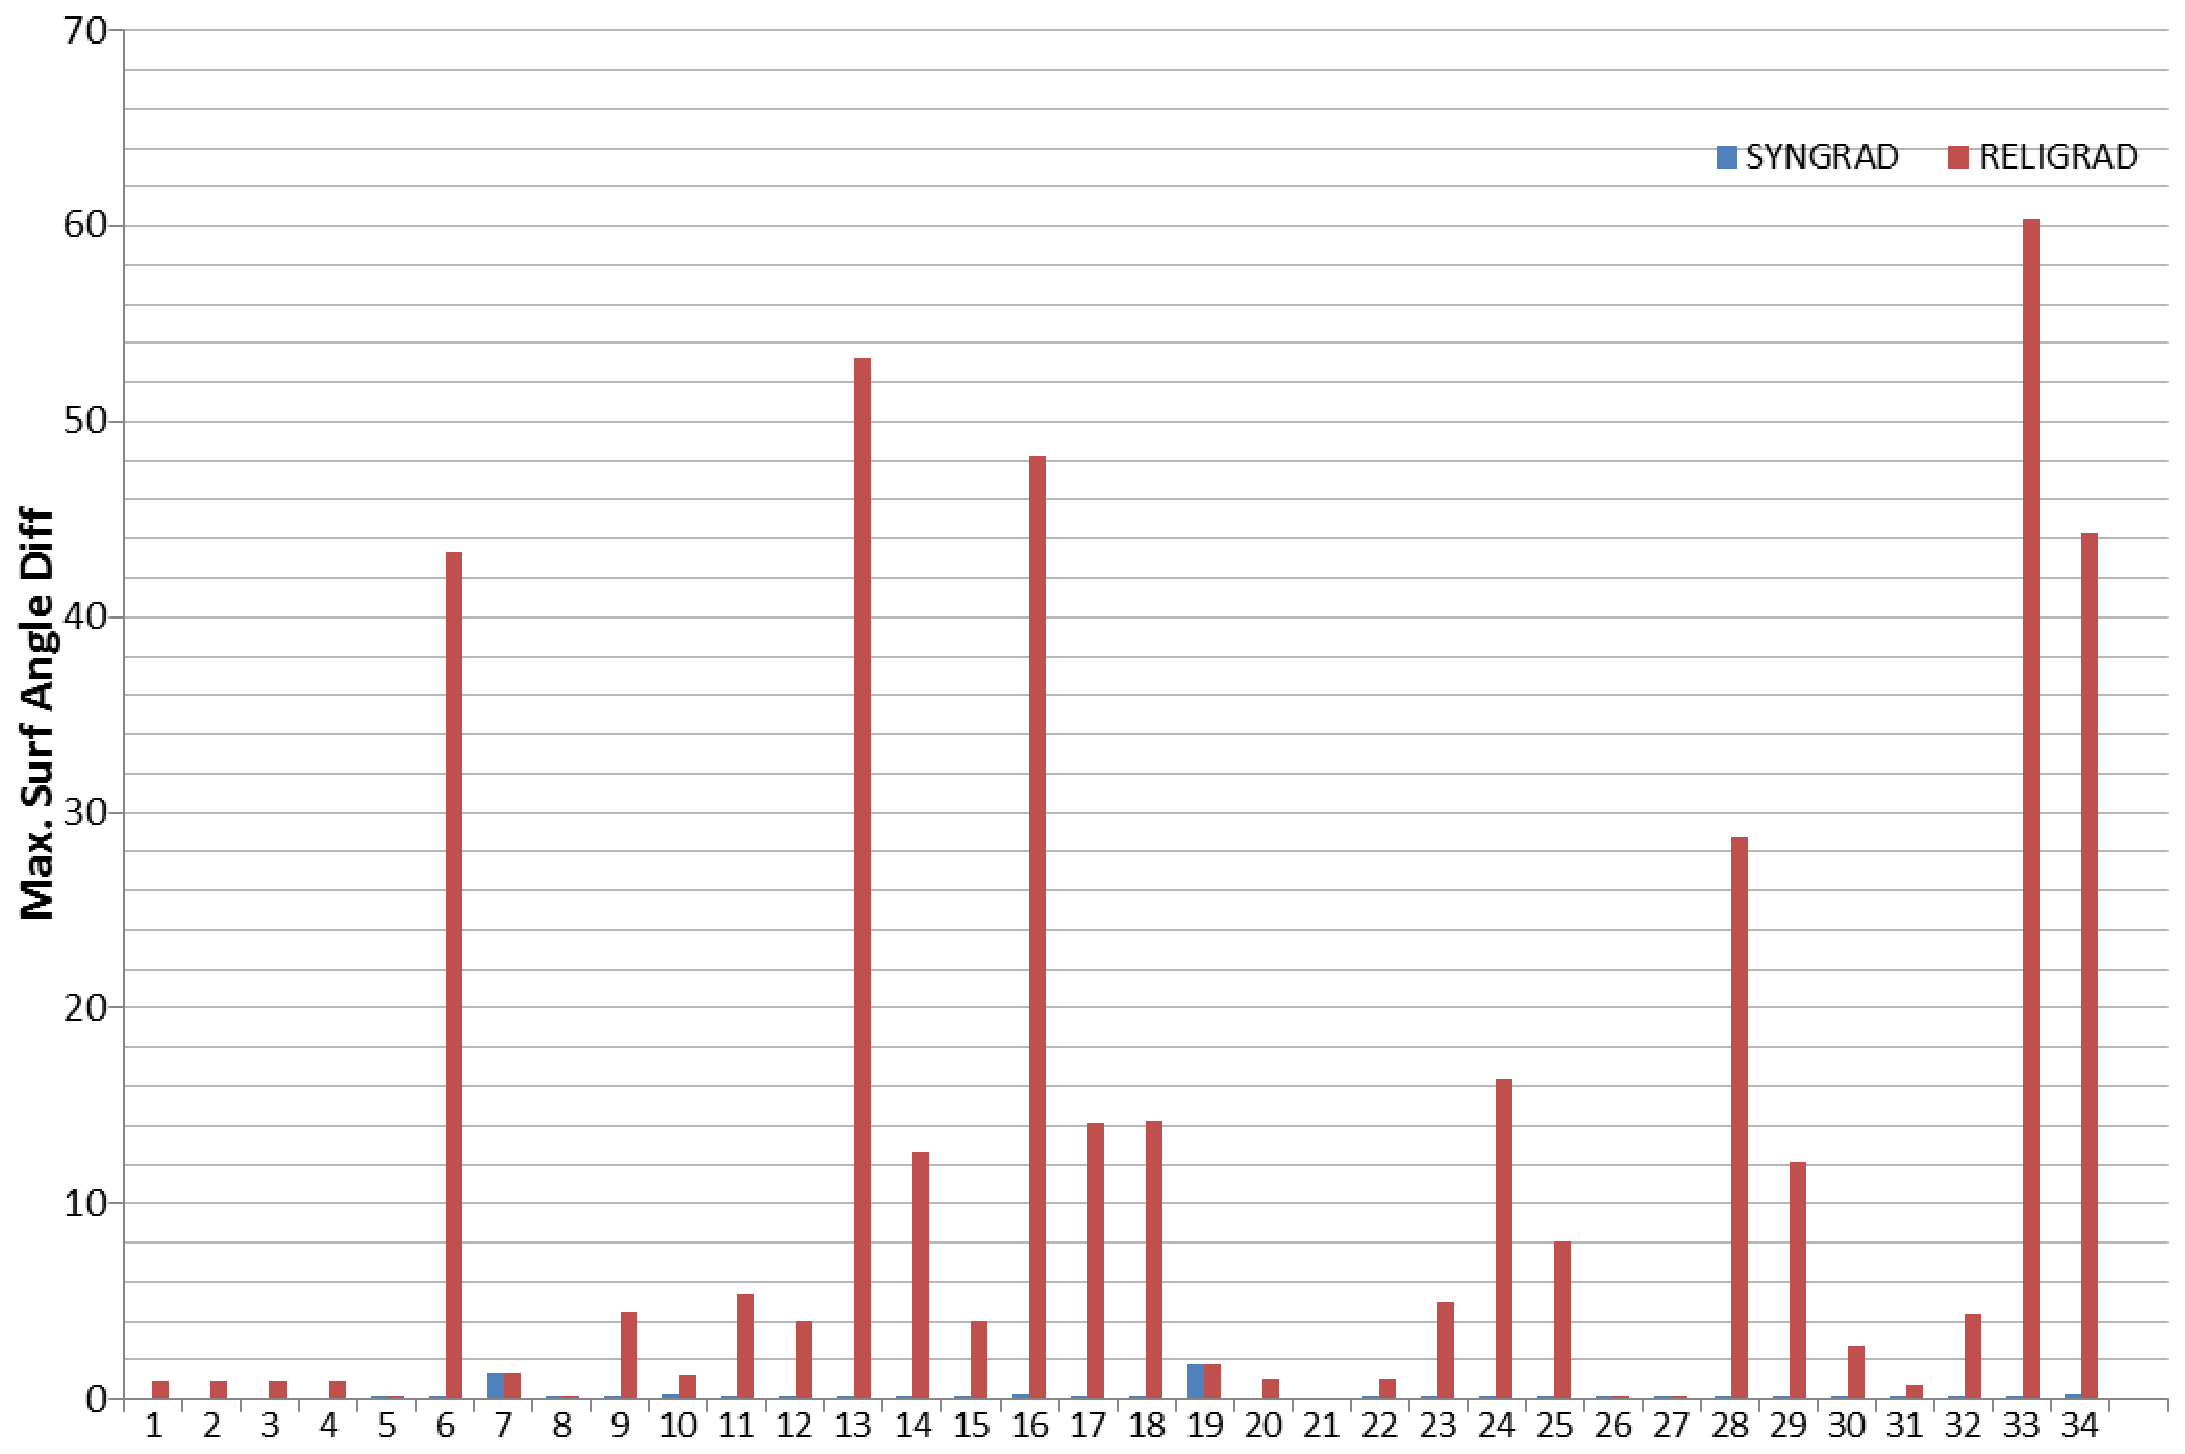
\includegraphics[width=0.3\linewidth]{images/twoCube_maxAngle_shrec.eps}\label{}}\\
	\subfloat[]{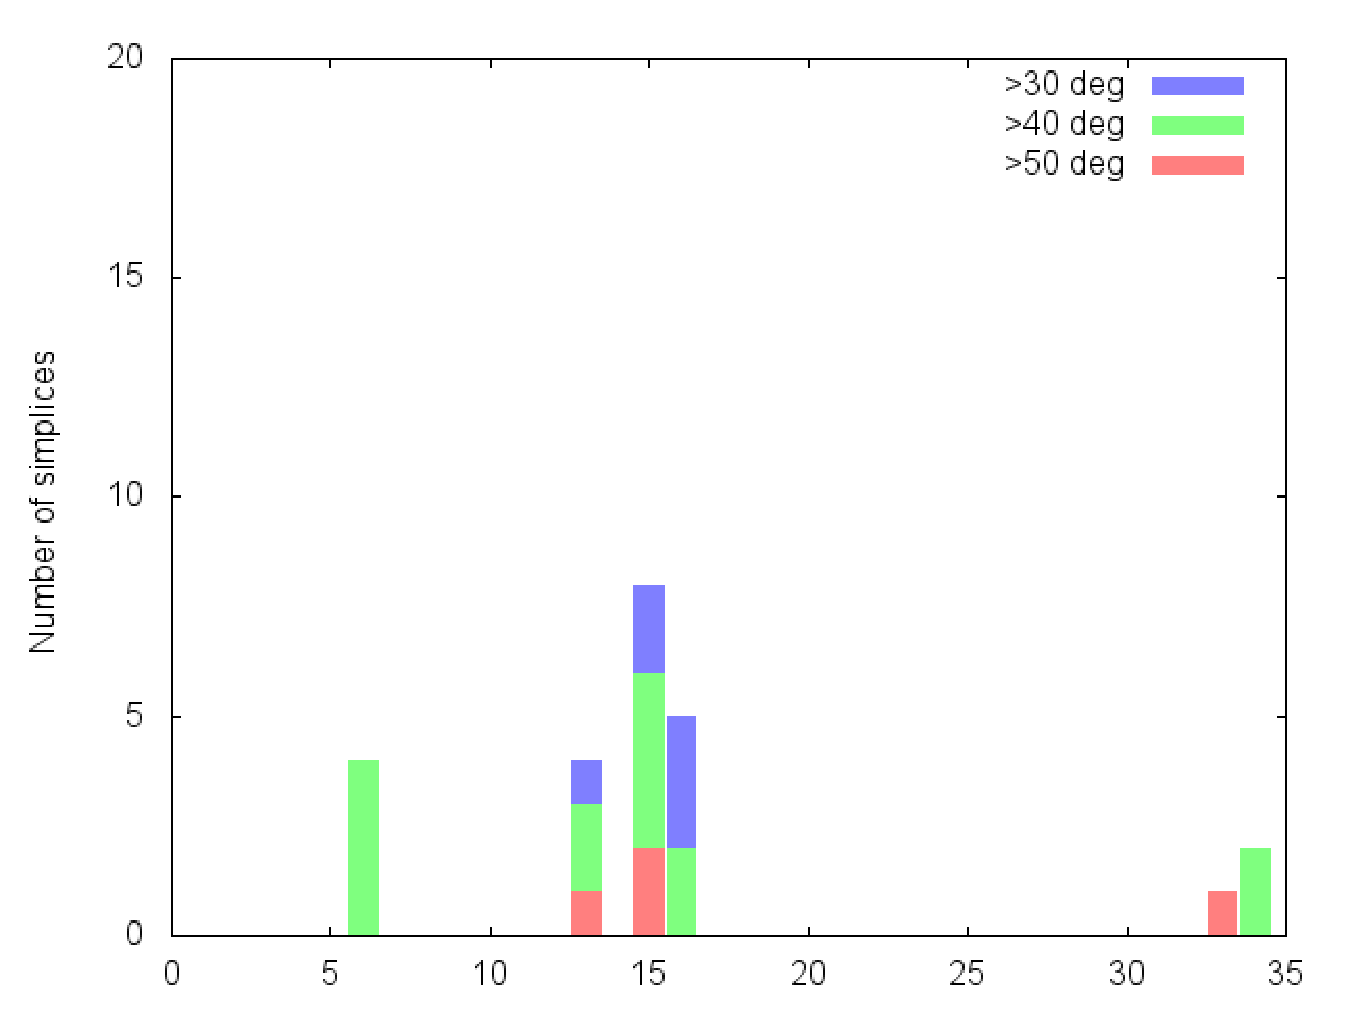
\includegraphics[width=0.3\linewidth]{images/twoCube_shrec_distribution.eps}\label{}}
%\begin{tabular}{cc}
%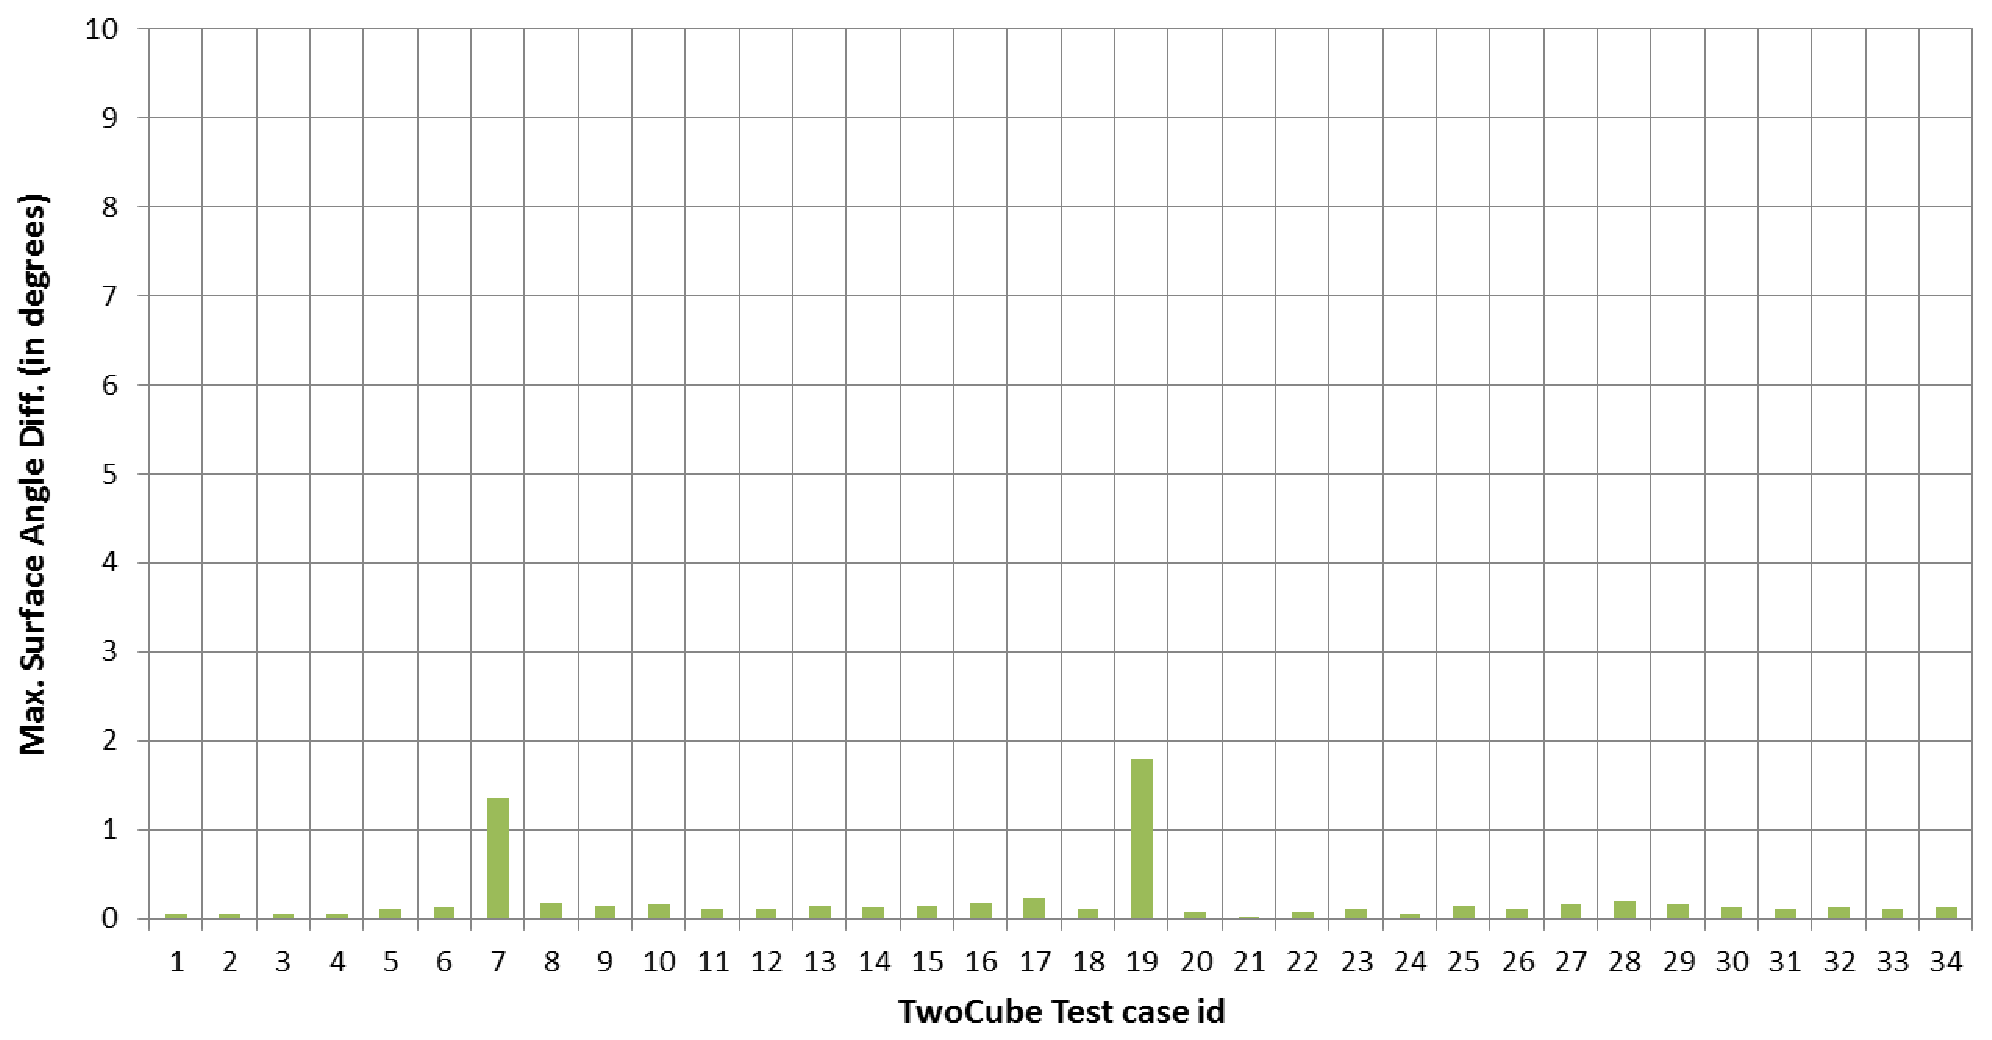
\includegraphics[width=0.45\linewidth]{images/tw1.eps} &
%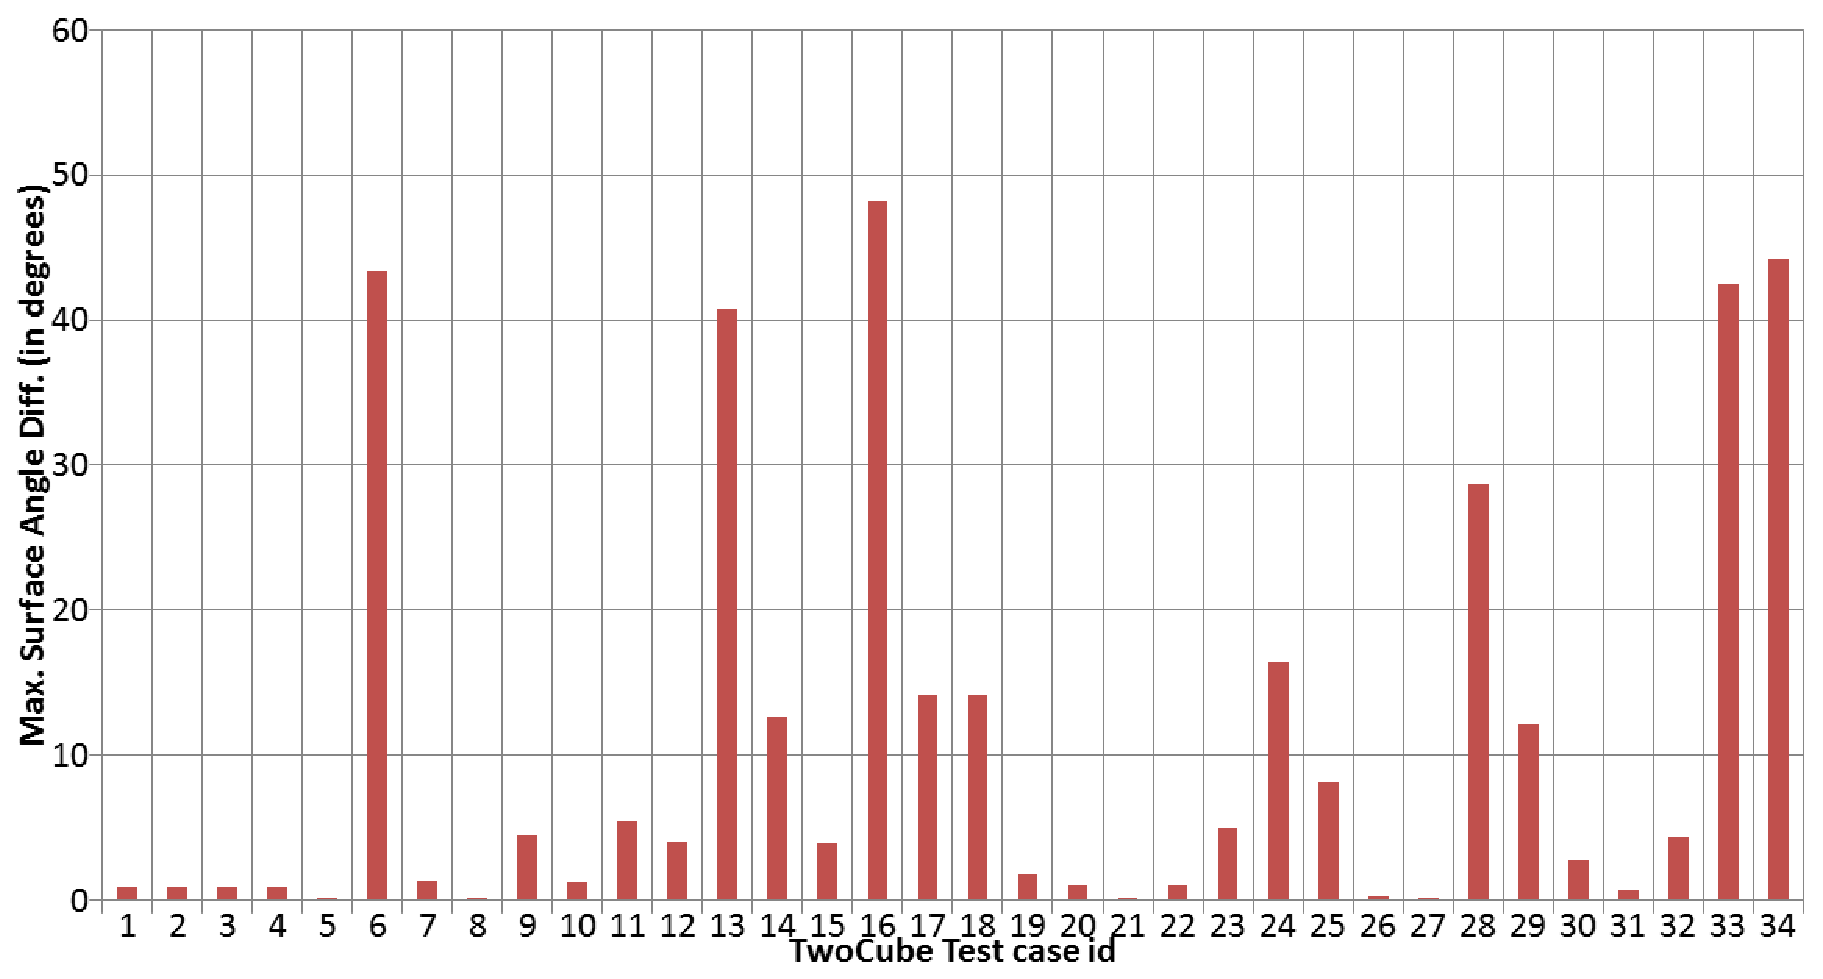
\includegraphics[width=0.45\linewidth]{images/tw2.eps} \\
%(a) SHREC using exact gradients & (b) SHREC using Religrad gradients \\
%\\
%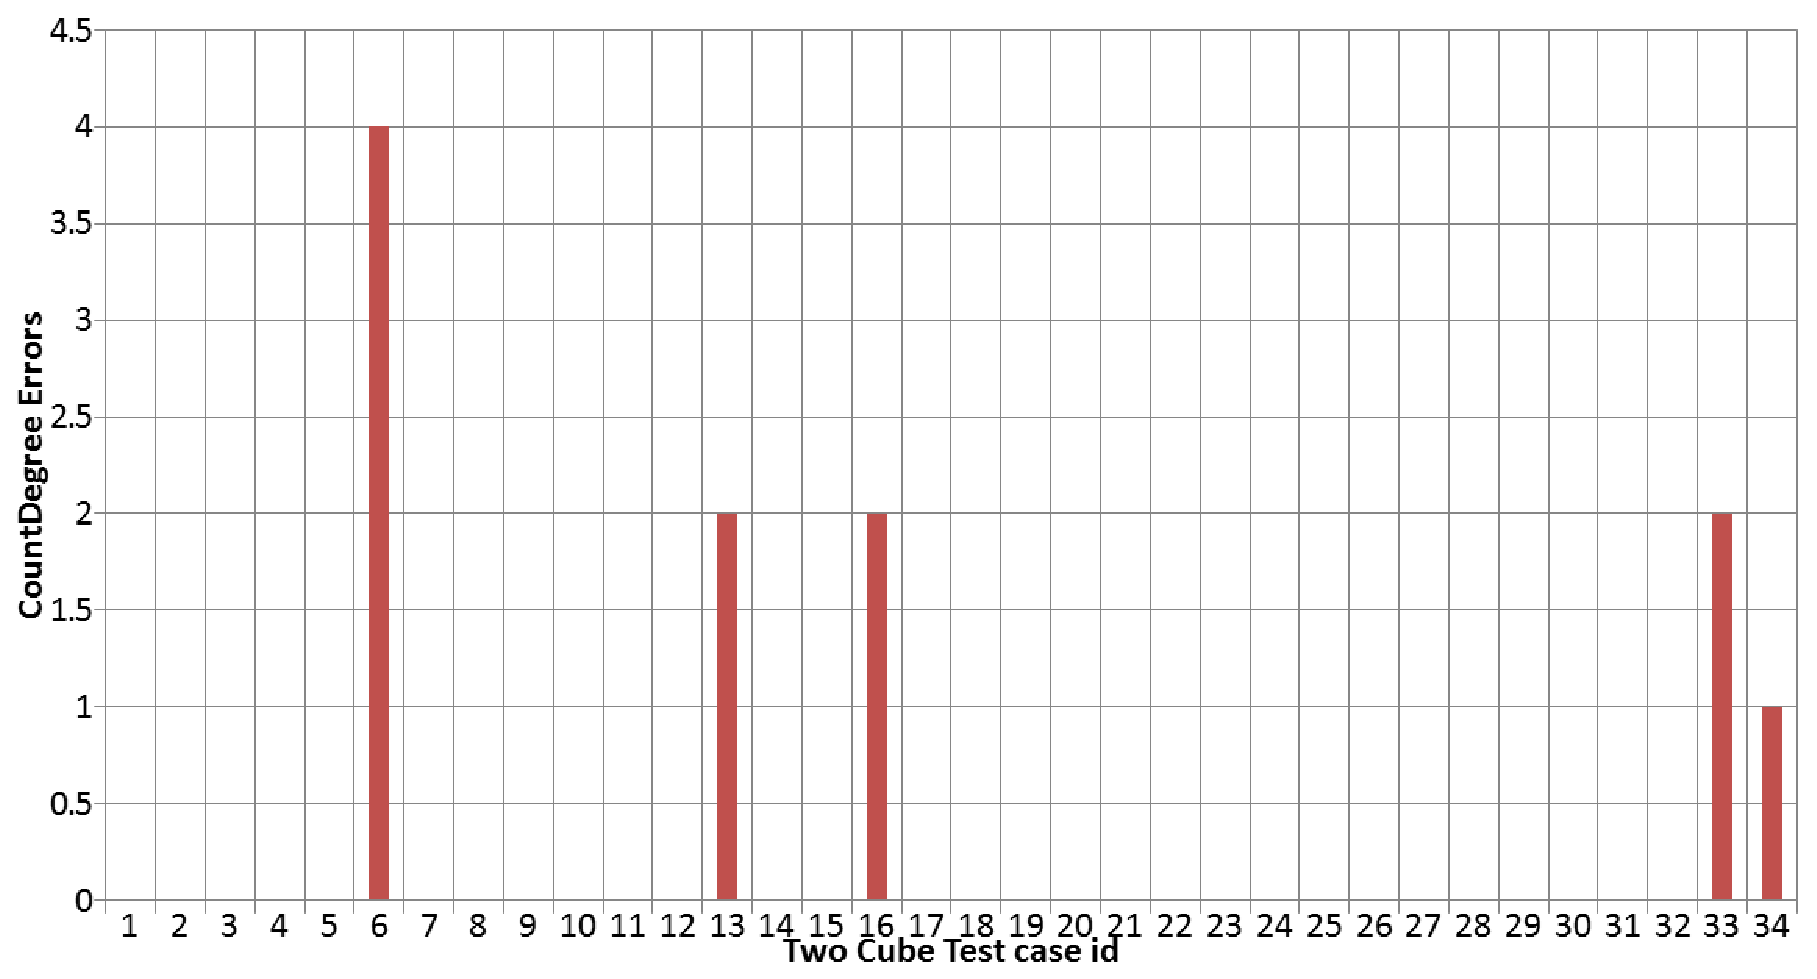
\includegraphics[height=0.25\linewidth]{images/tw3.eps} &
%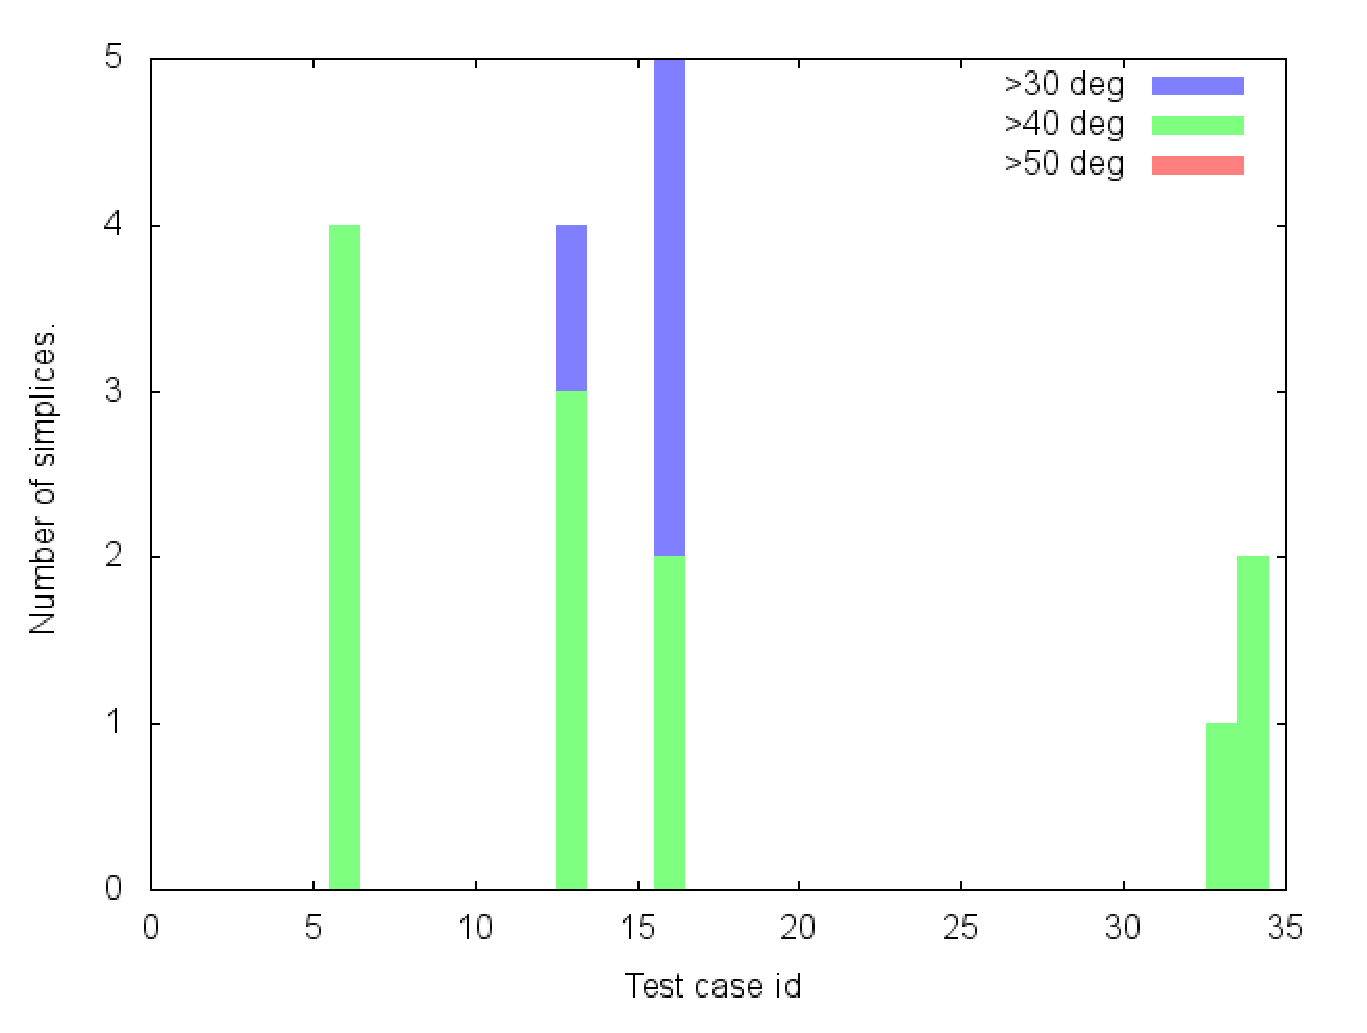
\includegraphics[height=0.25\linewidth]{images/twoCube35_test_1.eps} \\
%(c) Shrec using Religrad gradients & (d) SHREC using Religrad Gradients
%\end{tabular}

\caption{Results of SHREC using exact and Religrad gradients 
on 34 TwoCubes datasets. 
(a) Unoriented angle distance between isosurface (exact gradients)
and polygonal mesh.
(Note that the $y$-scale is from 0 to $10^\circ$.)
(b) Unoriented angle distance between isosurface (Religrad gradients)
and polygonal mesh.
(c)~Number of isosurface triangles (Religrad gradients)
with angle difference to polygonal mesh above 30, 40 and 50 degrees.
(d)~Number of degree errors in the 1-skeleton of sharp edges
(Religrad gradients).
(SHREC using exact gradients produces no degree errors.)}
\label{fig:shrecTwoCube}

\end{figure*}


\subsection{Isosurface Reconstruction on Synthetic Data}
\label{section:synthetic_tests}

We tested SHREC on 40 Flange datasets with 40 different orientations
and 34 TwoCubes datasets with 34 different orientations.
Table~\ref{table:datasets} presents dataset sizes, isovalues,
and average isosurface sizes.
We tested SHREC both on gradients produced by exact formulas 
and on gradients produced by ReliGrad.
We measured the unoriented angle distance between the SHREC isosurfaces
and the polygonal meshes representing the level sets.
We also counted the number of isosurface triangles whose normal differences
were above $30^\circ$, $40^\circ$ and $50^\circ$.
Finally, we measured the number of degree errors 
in the 1-skeleton of sharp isosurface edges.

Figure~\ref{fig:flange1} shows a Flange isosurface produced by SHREC
using exact gradients.
The magnified region shows edges with dihedral angle
less than $140^\circ$ in red blended with a subset of the ``non-sharp"
edges.

With exact gradients,
all the Flange isosurfaces had unoriented angle distance
under ??? from the polygonal meshes.
They also had no degree errors in the 1-skeletons
of sharp isosurface edges,
i.e. all the vertices in the 1-skeletons had degree two.

Figure~\ref{fig:flangeAngle} displays angle distance and degree error
information for the 40 Flange isosurfaces
when gradients were produced using Religrad.
As shown in Figure~\subref*{fig:flangeAngle1},
only one isosurface had triangles with angle distance greater than $50^\circ$
and less than half had no triangles with angle distance greater than $40^\circ$.
No isosurfaces had more than 5 triangles with angle distance
greater than $40^\circ$
and no isosurfaces had more than 15 triangles with angle distance greater
than $30^\circ$.

Figure~\subref*{fig:flangeAngle2} displays a histogram of angle distances
for a single Flange isosurface (id 17) 
whose gradients were produced using Religrad.
(Note the logarithmic scale.)
As can be seen,
there are very few triangles with angle distance
greater than $20^\circ$, $30^\circ$ or $40^\circ$.
The isosurface mesh has approximately 133
thousand triangles. 

Figure~\protect\subref*{fig:flangeAngle3} shows the 1-skeleton degree errors
for the 40 Flange isosurfaces when gradients were produced using Religrad.
Thirty two isosurfaces (80$\%$) had no degree errors.
No isosurface had more than eight degree errors.

Figure~\ref{fig:shrecPerfect1} shows a TwoCubes isosurface
and isosurface edges constructed by SHREC.
SHREC reproduces the 0-dimensional features with single mesh vertices
and the 1-dimensional features with a sequence of mesh edges
with dihedral angle $90^\circ$.

Figure~\ref{fig:shrecTwoCube} displays angle distance and degree error
information for the 34 TwoCube isosurfaces produced by SHREC.
Figure~\ref{fig:shrecTwoCube}(a) shows the unoriented angle distance
using exact gradients.
As with the exact gradients in the Flange datasets,
the angle distance is very low (less than $2^\circ$)
for all the isosurfaces.)
With exact gradients, the 34 TwoCubes isosurfaces 
had no 1-skeleton degree errors, 
i.e. they all had exactly 20 vertices with degree three 
in the 1-skeleton of their sharp edges.

Figure~\ref{fig:shrecTwoCube}(b) shows the unoriented angle distances
using gradients produced by Religrad.
For most isosurfaces, the angle distance is still low (under $10^\circ$),
although six isosurfaces have angle distances of between $30^\circ$
and $50^\circ$.
The high angle distances indicate errors in the SHREC reconstruction 
of sharp features.

For the isosurfaces constructed using Religrad gradients,
Figure~\ref{fig:shrecTwoCube}(c) gives
the number of isosurface triangles whose normal differences
are above $30^\circ$, $40^\circ$ and $50^\circ$.
Dataset 16, which had the largest angle distance over all 34 isosurfaces,
has only 5 triangles with normal difference more than 30$^\circ$ 
and a single triangle with normal distance over 40$^\circ$.  

Figure~\ref{fig:shrecTwoCube}(d) shows
the degree errors in the 1-skeleton of sharp edges
when gradients were produced using Religrad.
29 out of the 34 TwoCubes isosurfaces had no degree errors.
Of the 5 isosurfaces with degree errors,
the maximum number of degree errors was four.
As previously noted,
there were no degree errors for any of the 34 TwoCubes isosurfaces
when SHREC used exact gradients.

\begin{figure}[t]
	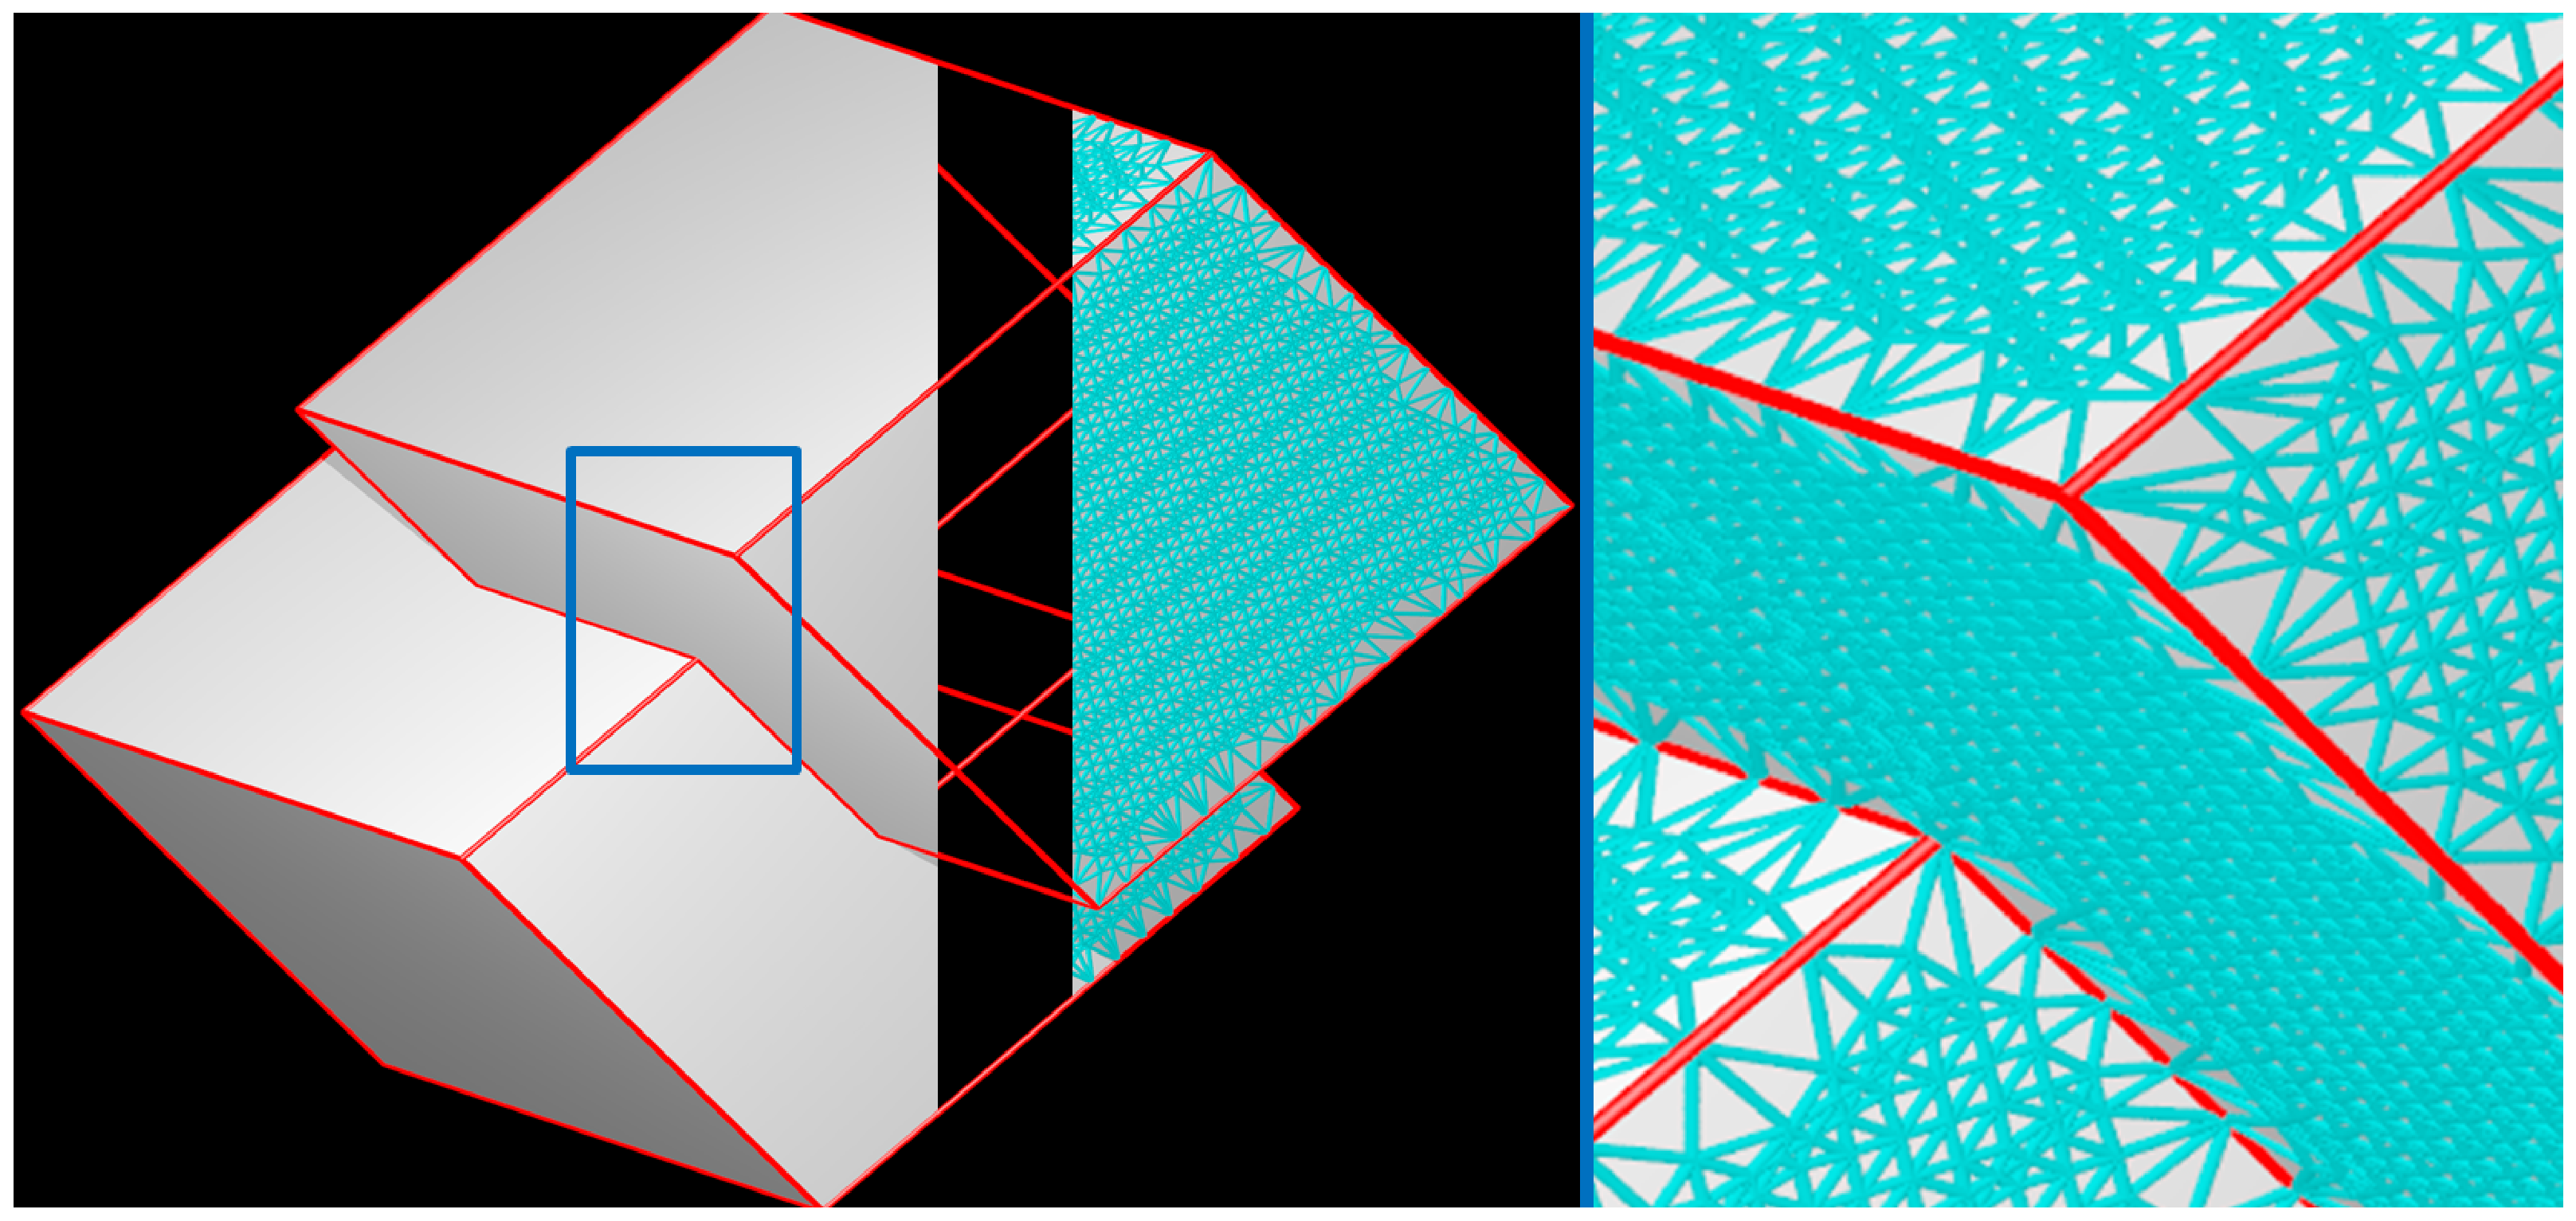
\includegraphics[width=\linewidth]{images/shrecPerfect.eps}
	\caption{SHREC TwoCubes isosurface. 
``Sharp" edges (dihedral angle less than $140^\circ$) are marked in red. 
Smooth edges are shown in cyan. The magnified region shows the output mesh edges around a corner.}
	\label{fig:shrecPerfect1}
\end{figure}

\begin{figure}[t]
\subfloat[Cannon]{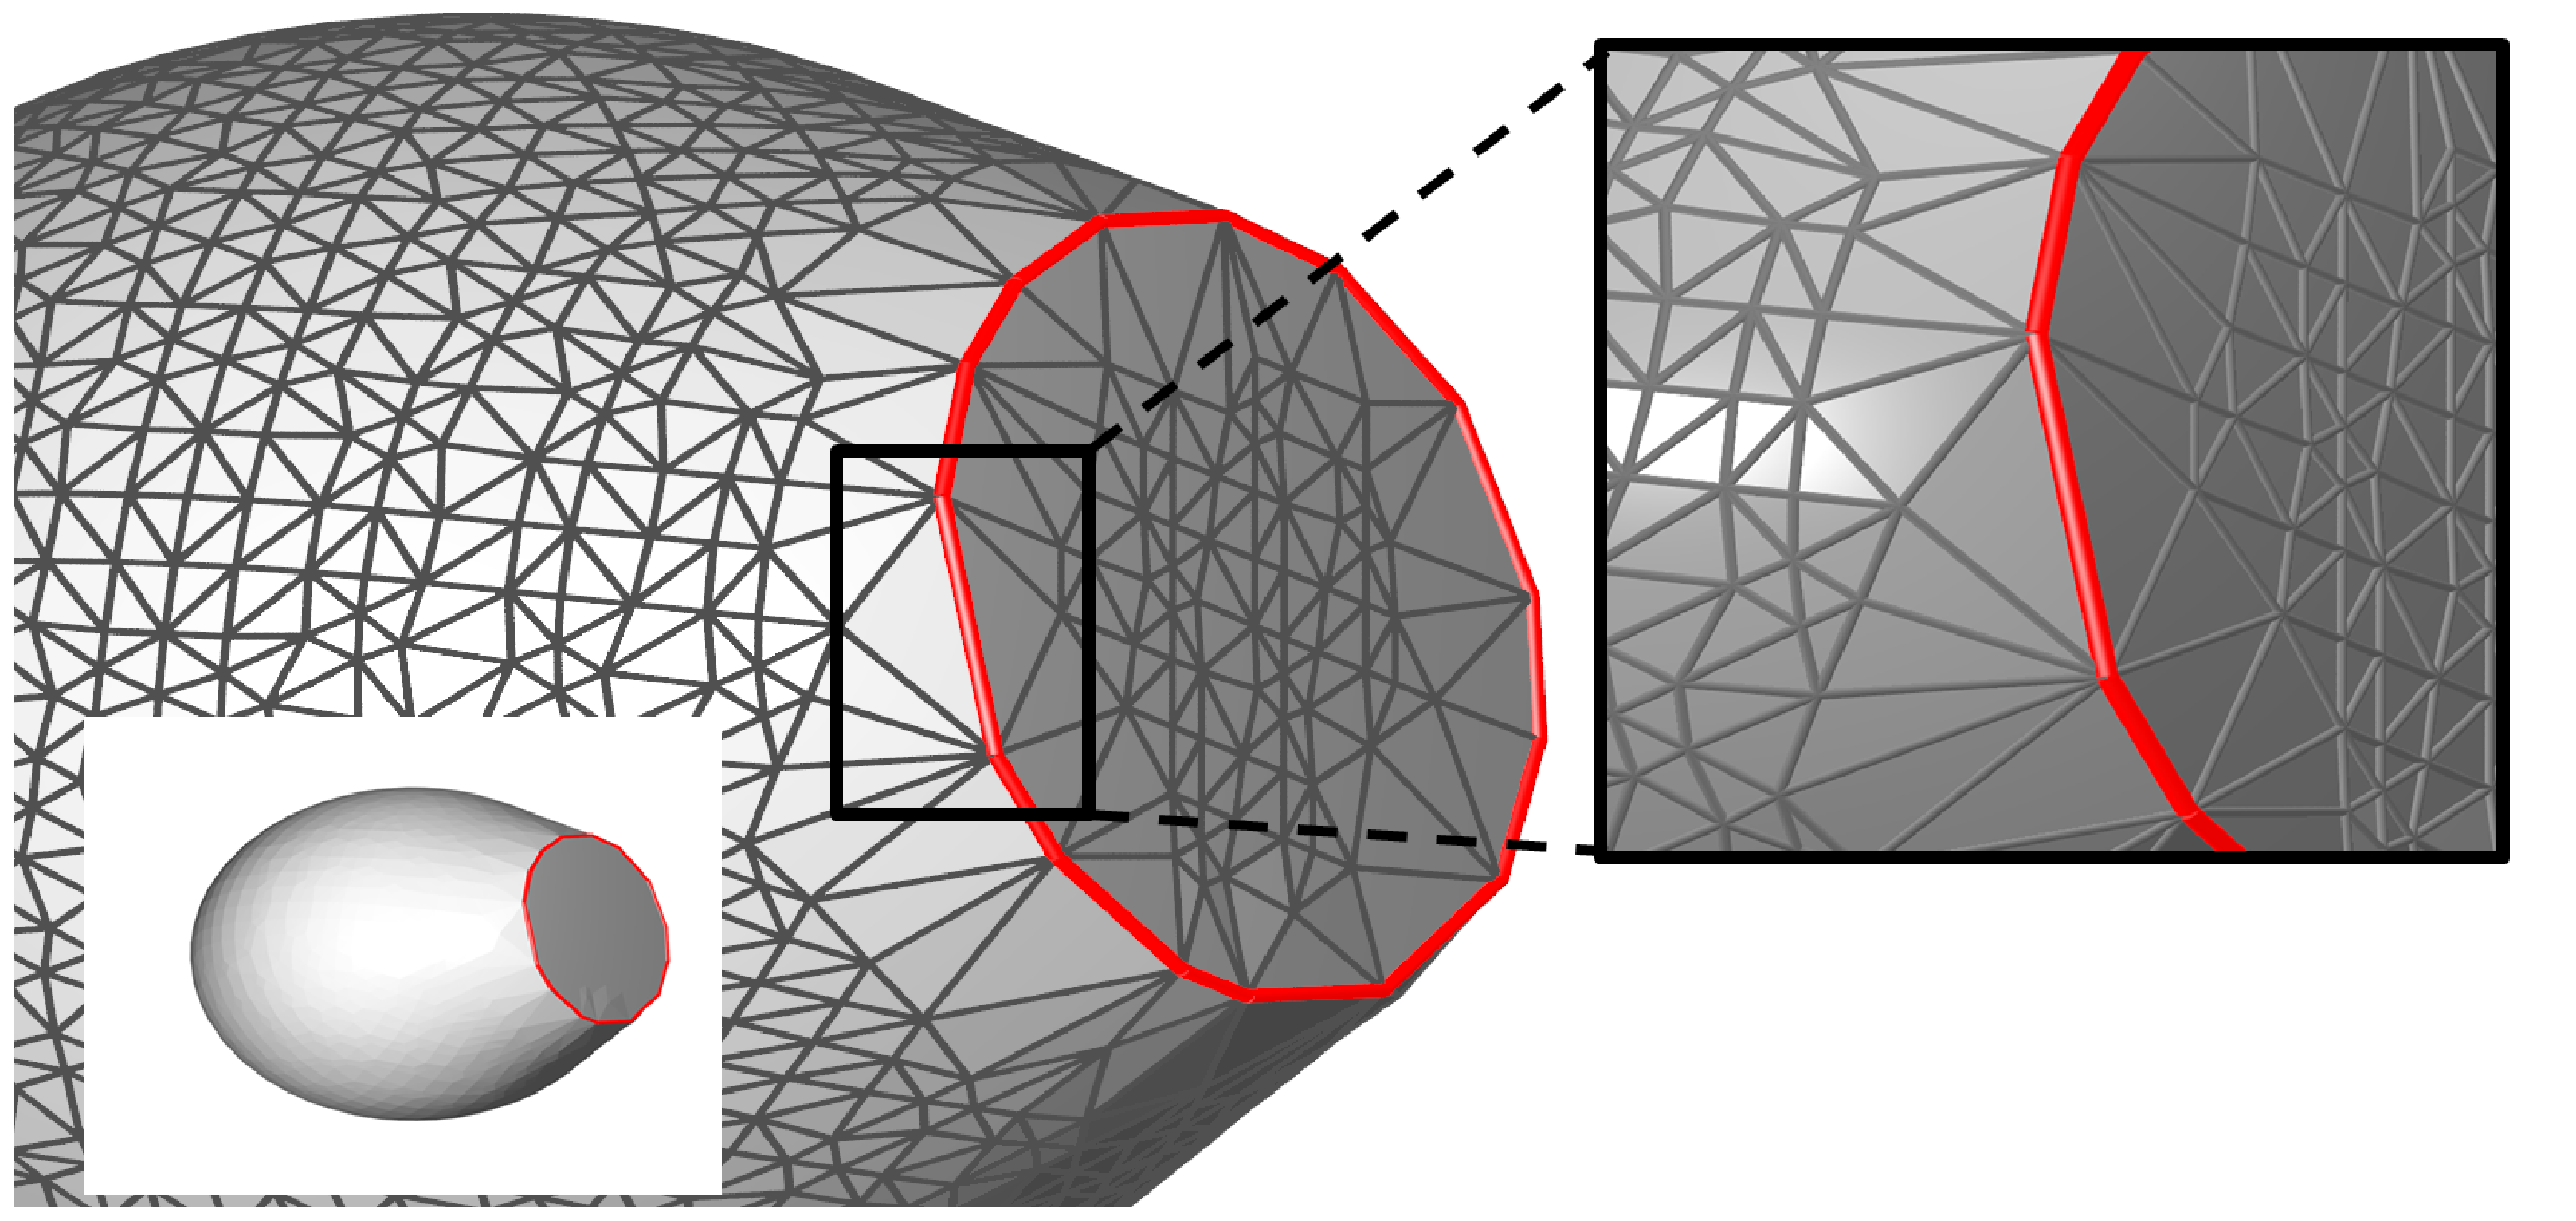
\includegraphics[width=0.5\linewidth]{images/cannon2.eps}\label{fig:cannon:a}}
\subfloat[Smooth Tip Cone]{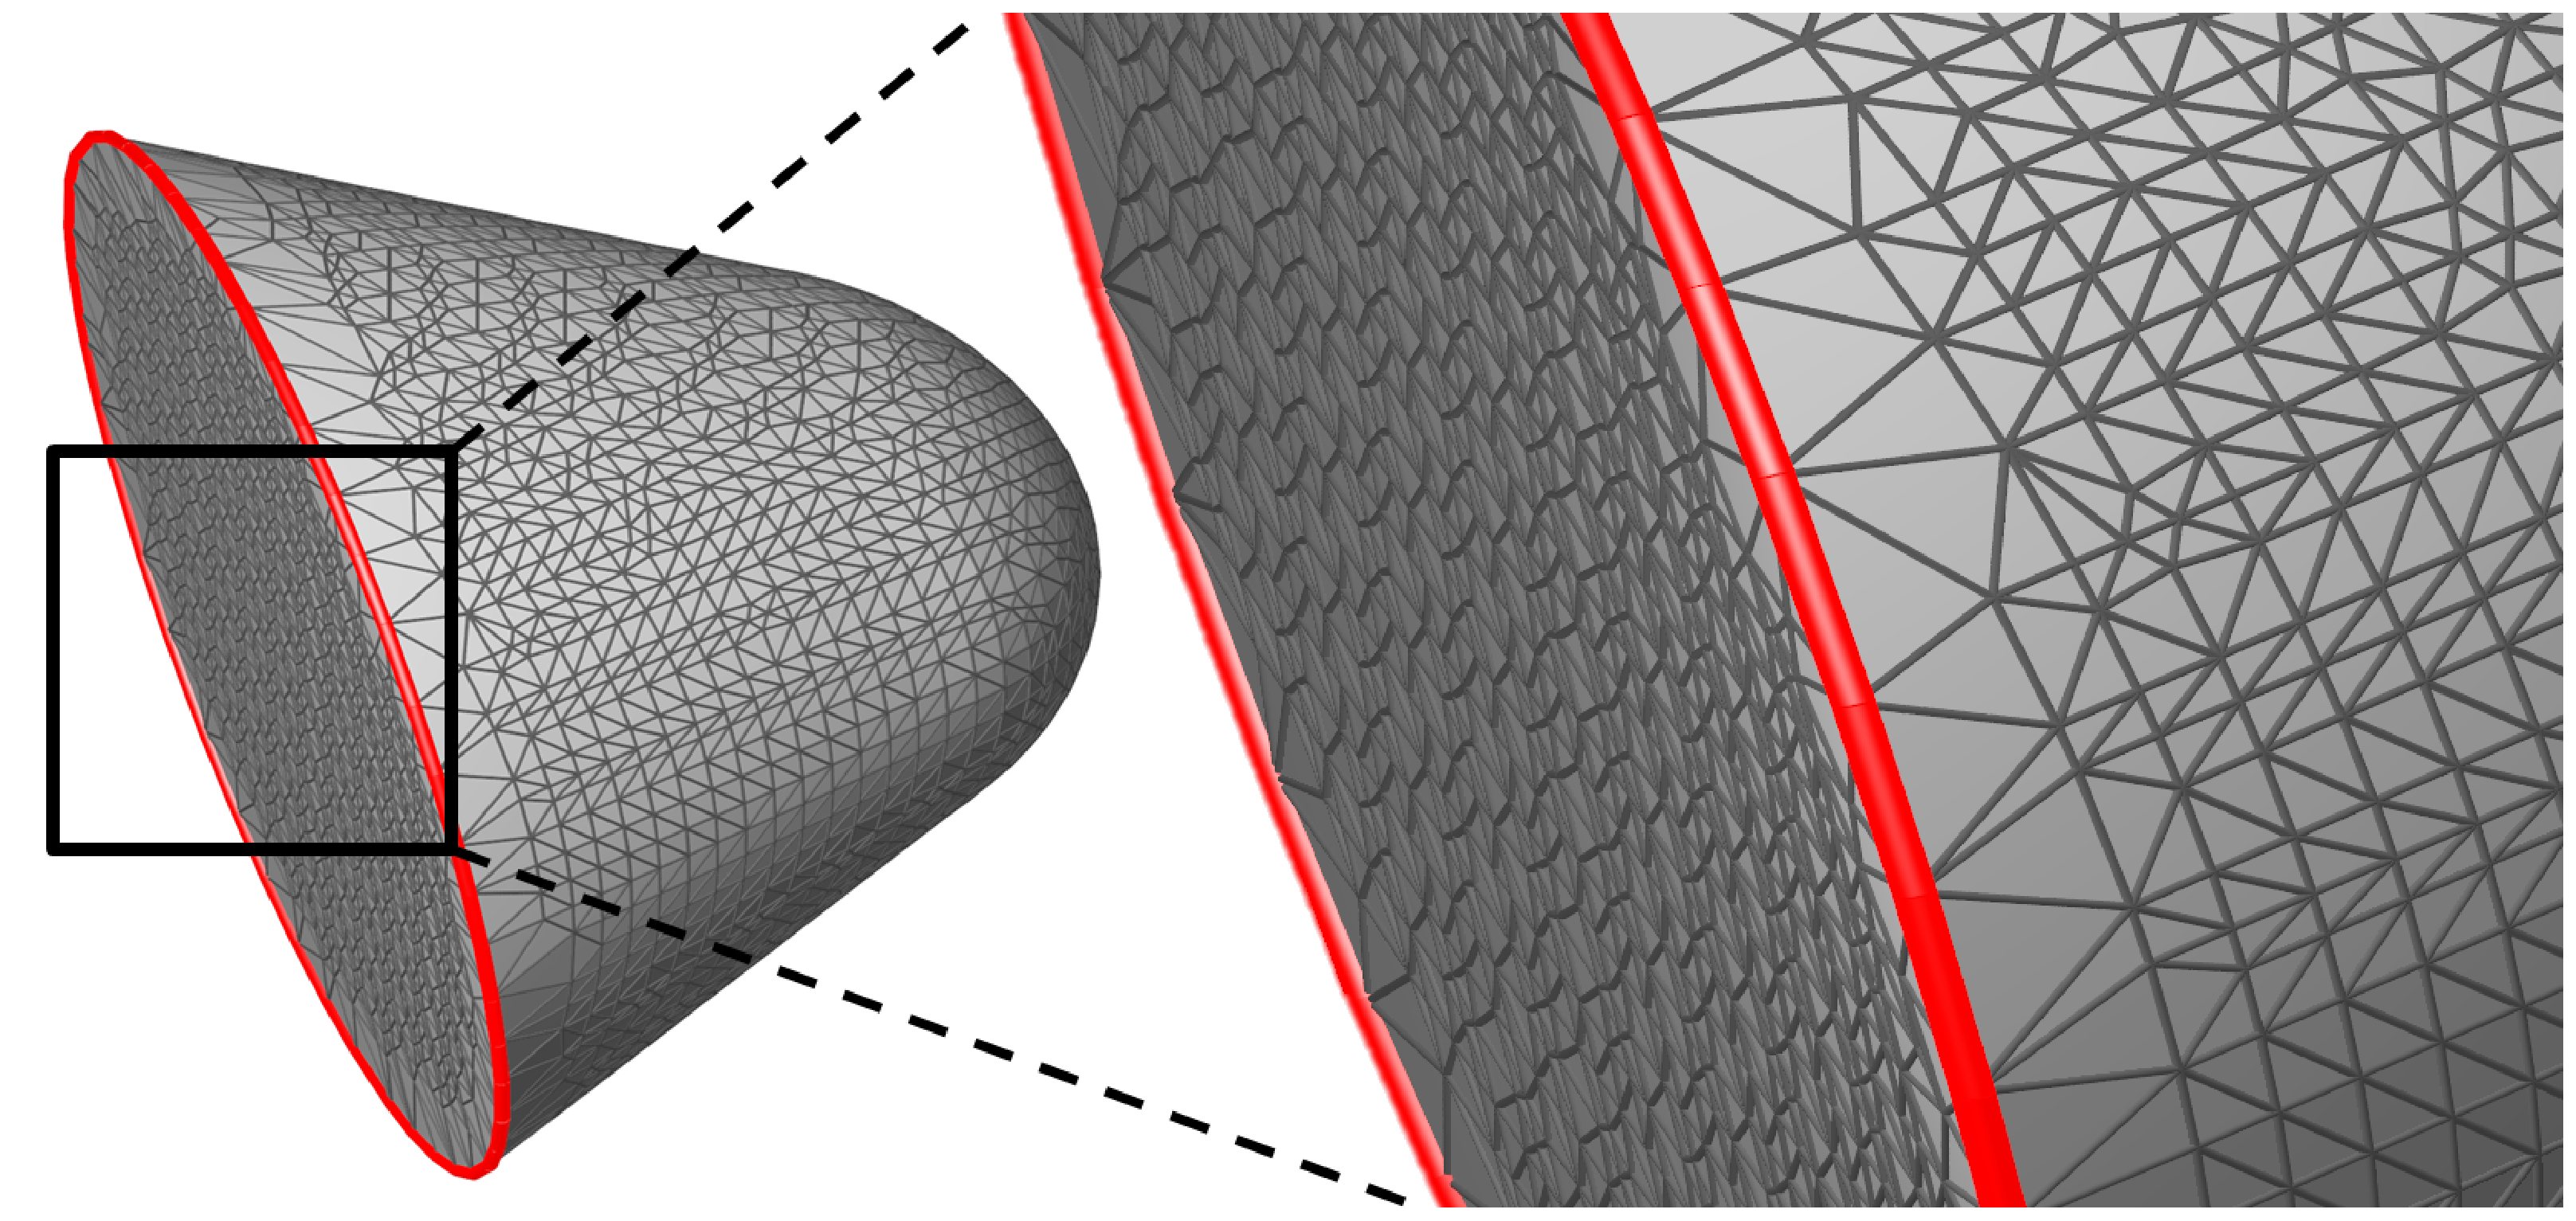
\includegraphics[width=0.5\linewidth]{images/cone2.eps}\label{fig:cone:a}}
\caption{SHREC Cannon and Smooth Tip Cone isosurfaces (Religrad gradients.) 
(a)~Cannon isosurface.
\mbox{1-dimensional} feature has dihedral angle $120^\circ$.
(b)~Smooth Tip Cone isosurface.  1-dimensional feature has dihedral angle $60^\circ$.}
\label{fig:cannon_cone}
\end{figure}

\begin{figure}[t]
	\subfloat[]{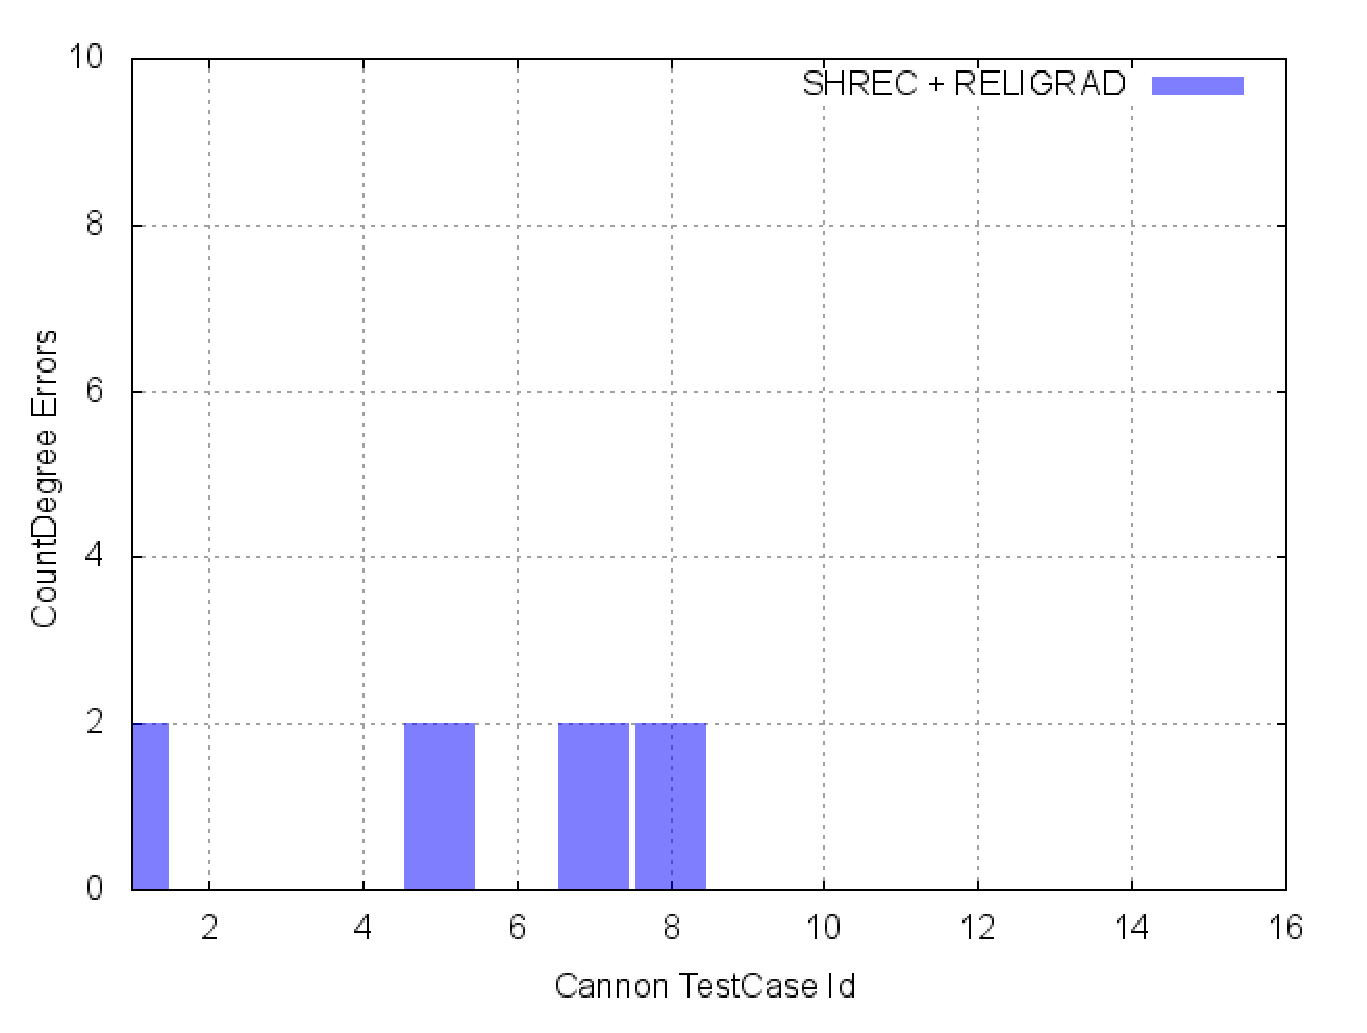
\includegraphics[width=0.5\linewidth]{images/cannon.eps}\label{fig:cannon:b}}
	\subfloat[]{\includegraphics[width=0.5\linewidth]{images/cone.eps}\label{fig:cone:b}}

\caption{Results of SHREC on 15 Cannon and 14 Smooth Tip Cone datasets.
(a) Number of degree errors on 1-skeleton of Cannon isosurfaces
constructed using Religrad gradients.
(Cannon isosurfaces constructed using exact gradients had no degree errors.)
(b) Number of degree errors on 1-skeleton of Smooth Tip Cone isosurfaces
constructed using Religrad gradients (green) and exact gradients (red).}
\label{fig:cannon_cone_summary}
\end{figure}

\begin{table*}[t]
\centering
\begin{tabular}{|l|l|l|c|}
\hline
Software & Algorithm & URL & References \\
\hline
EMC (IsoEx) & Extended Marching Cubes &
\href{https://www.graphics.rwth-aachen.de/software}{www.graphics.rwth-aachen.de/software} & \cite{kbsh-fssev-01} \\
\hline
EMCpoly & Extended Marching Cubes &
\href{http://web.cse.ohio-state.edu/research/graphics/isotable}{web.cse.ohio-state.edu/research/graphics/isotable} & \\
\hline
PolyMender & Dual Contouring &
\href{http://www.cse.wustl.edu/~taoju/code/polymender.htm}{www.cse.wustl.edu/~taoju/code/polymender.htm} & \cite{j-rrpm-04,jlsw-dchd-02,sw-dcss-02} \\
\hline
SingularCocone & &
\href{http://web.cse.ohio-state.edu/~tamaldey/cocone.html}{web.cse.ohio-state.edu/~tamaldey/cocone.html} & \cite{cdr-drpsc-07,Dey2012,Dey2013} \\
\hline
MergeSharp & &
\href{http://web.cse.ohio-state.edu/research/graphics/isotable}{web.cse.ohio-state.edu/research/graphics/isotable} & \cite{bw-cisec-13,bw-erm-13}\\
\hline
SHREC & &
\href{http://web.cse.ohio-state.edu/research/graphics/isotable}{web.cse.ohio-state.edu/research/graphics/isotable} & \\
\hline
\end{tabular}

\caption{Surface reconstruction software.
EMC is a sample implementation of Extended Marching Cubes.
EMCpoly is a modification of EMC which creates TwoCubes and Flange isosurfaces.
PolyMender is an implementation of dual contouring for fixing polygonal meshes.
SingularCocone is an implementation of a Voronoi based algorithm
for surface reconstruction from point clouds.
The algorithm handles 0 and 1 dimensional features
including non-manifold features.
MergeSharp is an implementation of a dual contouring reconstruction algorithm 
which uses cube merging to obtain better reconstruction around sharp features.
SHREC is an implementation of the algorithm in this paper.}
\label{table:software}
\end{table*}

To measure the dihedral angles other than $90^\circ$,
we ran SHREC on 15 Cannon datasets with 15 different orientations
and 14 Smooth Tip Cone datasets with 14 different orientations.
The 1-dimensional features in the Cannon level sets
had dihedral angles of $60^\circ$.
The 1-dimensional features in the Smooth Tip Cone level sets
had dihedral angles of $120^\circ$.
As expected, SHREC produced more errors than on the Flange or TwoCube
datasets, although it still did quite well.

Figure~\ref{fig:cannon_cone} shows Cannon and Smooth Tip Cone isosurfaces
produced by SHREC using Religrad gradients.
In each, the 1-dimensional is represented by a sequence 
of isosurface mesh edges with the appropriate dihedral angles.

Figure~\ref{fig:cannon_cone_summary} gives the number of degree errors
in the 1-skeleton of sharp edges
for Cannon and Smooth Tip Cone isosurfaces.
SHREC using exact gradients produced no degree errors 
on the 15 Cannon datasets.
SHREC using Religrad produced degree errors on only four Cannon datasets.
For each dataset, there were exactly two degree errors.
SHREC using exact gradients produced degree errors in only two 
of the Smooth Tip Cone datasets,
one with two errors and one with four.
SHREC using Religrad gradients produced degree errors on 7 out of the 14
Smooth Tip Cone datasets.
The maximum number of degree errors in any Smooth Tip Cone isosurface
was 4.



\begin{figure*}[p]
\centering

\begin{tabular}{cc}
	\subfloat[Flange: Angle distance]{\includegraphics[width=0.45\linewidth]{images/ms_euro_flange_maxAngle.eps}\label{fig:msharp:flange:A}} &
	\subfloat[Flange: Degree errors]{\includegraphics[width=0.45\linewidth]{images/ms_euro_flange_countDegree.eps}\label{fig:msharp:flange:D}} \\
	\subfloat[TwoCubes: Angle distance]{\includegraphics[width=0.45\linewidth]{images/ms_euro_twoCube_maxAngle.eps}\label{fig:msharp:tc:A}} &
	\subfloat[TwoCubes: Degree errors]{\includegraphics[width=0.45\linewidth]{images/ms_euro_twoCube_countDegree.eps}\label{fig:msharp:tc:D}} \\
	\subfloat[Flange: Triangle normal differences]{\includegraphics[width=0.45\linewidth]{images/ms_euro_flange_distribution.eps}\label{fig:msharp:flange:c}} &
	\subfloat[TwoCubes: Triangle normal differences]{\includegraphics[width=0.45\linewidth]{images/ms_euro_twoCube_distribution.eps}\label{fig:msharp:tc:c}} 
%\\
%	\subfloat[Notch in MergeSharp Flange isosurface]{\includegraphics[width=0.3\linewidth]{images/mergeSharpvsShrec2.eps}\label{fig:msharp:b}} &
%	\subfloat[Dimpled MergeSharp isosurface (left) and smooth SHREC isosurface (right)]{\includegraphics[width=0.3\linewidth]{images/cone_mergesharp.eps}\label{fig:msharp:c}}
\end{tabular}
	\caption{Results of  MergeSharp on 40 Flange and 34 TwoCubes datasets
(exact gradients).
	\protect\subref{fig:msharp:flange:A}~Angle distance to polygonal Flange meshes.
	\protect\subref{fig:msharp:flange:D}~Degree errors in 1-skeleton 
of sharp edges of Flange datasets.
	\protect\subref{fig:msharp:tc:A}~Angle distance to polygonal TwoCubes meshes.
	\protect\subref{fig:msharp:tc:D}~Degree errors in 1-skeleton 
of sharp edges of TwoCubes datasets.
	\protect\subref{fig:msharp:tc:c}~Number of triangles 
with angle difference to polygonal Flange mesh above 30, 40 and 50 degrees.
(No Flange isosurface triangles have angle difference above $50^\circ$.)
	\protect\subref{fig:msharp:flange:c}~Number of triangles 
with angle difference to polygonal TwoCubes mesh above 30, 40 and 50 degrees.
}
\label{fig:msharp}
\end{figure*}	

\begin{figure*}[t]
\centering
\begin{tabular}{cc}
\subfloat[Notch in MergeSharp Flange isosurface]{\includegraphics[width=0.4\linewidth]{images/mergeSharpvsShrec2.eps}\label{fig:msharp:b}} \quad &
\quad
\subfloat[Dimpled MergeSharp isosurface (left) and smooth SHREC isosurface (right)]{\includegraphics[width=0.4\linewidth]{images/cone_mergesharp.eps}\label{fig:msharp:c}}
\end{tabular}

\caption{
\protect\subref{fig:msharp:b}~Notch in a MergeSharp Flange isosurface.
\protect\subref{fig:msharp:c}~Dimples in a MergeSharp Cone isosurface (left).
Compare with smooth SHREC isosurface (right).}

\end{figure*}


\section{Comparison with Other Algorithms}
\label{section:comparison}

We compared SHREC with software implementations of four other algorithms:
MergeSharp~\cite{bw-cisec-13,bw-erm-13}, 
PolyMender~\cite{j-rrpm-04}, 
EMC (Extended Marching Cubes)~\cite{kbsh-fssev-01} 
and SingularCocone~\cite{Dey2012}.
Table~\ref{table:software} contains descriptions of the software.

Input to both SHREC and MergeSharp is a regular grid sampling
of a scalar field and the gradients at the grid vertices.
Input to the software implementations of the other algorithms
is very different from input to SHREC or inputs to each other,
so one should be extremely careful in make comparisons
between these algorithms based on the results presented here.
For instance, on average,
EMC has fewer degree errors
than PolyMender or SingularCocone,
but EMC computes scalar, 
distance and normal values from formulas hard coded into the software.
PolyMender and SingularCocone (and SHREC and MergeSharp)
would certainly do much better if their input came
from formulas hard coded into their software.

SingularCocone has the most degree errors,
but SingularCocone is designed for reconstruction 
from point samples of a (possibly non-manifold) surface,
not for reconstruction from sampling of a scalar field.
Input to SingularCocone is point samples of a surface,
not scalar grid or gradient information.


\begin{figure*}[t]
	\centering
			\subfloat[PolyMender Flange isosurface]{\includegraphics[width=0.33\linewidth]{images/polymender4.eps}\label{fig:polymenderB:b}}\quad
			\subfloat[SHREC Flange isosurface]{\includegraphics[width=0.33\linewidth]{images/polymender3.eps}\label{fig:polymenderB:a}}
			\subfloat[Triangle normal differences]{\includegraphics[width=0.3\linewidth]{images/polymenderHistogram_1.eps}\label{fig:polymenderB:c}}\\
			\subfloat[PolyMender]{\includegraphics[width=0.2\linewidth]{images/polymender_cone_merge_2.eps}\label{fig:polymender:cone:b}}\qquad
			\subfloat[SHREC]{\includegraphics[width=0.2\linewidth]{images/polymender_cone_merge_1.eps}\label{fig:polymender:cone:a}}\qquad
			\subfloat[Magnified Smooth Tip Cone isosurfaces]{\includegraphics[width=0.4\linewidth]{images/polymender_cone_merge_3.eps}\label{fig:polymender:cone:c}}

\caption{PolyMender and SHREC comparison.
Mesh edges with dihedral angle below $140^\circ$ are colored red.
\protect\subref{fig:polymenderB:b}~PolyMender Flange isosurface.
\protect\subref{fig:polymenderB:a}~Corresponding SHREC Flange isosurface.
\protect\subref{fig:polymenderB:c} Distribution of differences of triangle normals
between PolyMender isosurface and polygonal mesh (red)
and between SHREC isosurface and polygonal mesh (green).
\protect\subref{fig:polymender:cone:b} PolyMender Cone isosurface.
\protect\subref{fig:polymender:cone:a} Corresponding SHREC Cone isosurface.
\protect\subref{fig:polymender:cone:c} Magnified view of Polymender isosurface (left)
and corresponding SHREC isosurface (right).
} 
\label{fig:polymenderB}
\end{figure*}


\paragraph{Comparison with MergeSharp.}

%mergesharp_euro =['E:\\Programs\\Win\\stdAlone\\ijk\\bin\\mergesharpbin\\Release\\mergesharp.exe', '-position', 'gradNS', '-trimesh']
%def compare_with_euro(n, iso):

Input to MergeSharp is a regular grid sampling of a scalar field
and the gradients at the grid vertices.
We ran MergeSharp on the same 40 Flange and 34 TwoCube synthetic datasets
that we applied to SHREC in Section~\ref{section:synthetic_tests}.
We used the exact gradients on MergeSharp, not the Religrad gradients.
Figures~\subref*{fig:msharp:flange:A} and~\subref*{fig:msharp:tc:c}
shows the oriented angle distance between the MergeSharp isosurfaces 
and the polygonal mesh isosurfaces.
Five of the MergeSharp TwoCubes isosurfaces have angle distance 
near $180^\circ$ indicating ``flipped'' triangles produced by folds
in the mesh.
Figures~\ref{fig:msharp:flange:c} and~\ref{fig:msharp:tc:c} 
present the number of triangles with angle difference greater
than $30$, $40$ and $50$ degrees 
in the MergeSharp Flange and TwoCubes isosurfaces.
24 out of 40 of the Flange isosurfaces and 18 out of 34 
of the TwoCube isosurface have angle distance above $30^\circ$
indicating significant problems in the reconstruction of sharp features.

Figures~\subref*{fig:msharp:flange:D} and~\subref*{fig:msharp:tc:D}
gives the number of degree errors in the 1-skeleton's of the sharp edges.
8 out of 40 of the Flange isosurfaces and 15 out of 34 of the TwoCube
isosurfaces have degree errors.
The maximum number of degree errors is eight.

Note that all the results in Figure~\ref{fig:msharp} are
for MergeSharp isosurfaces produced from EXACT gradients.
Thus, they should not be compared with the SHREC results
in Figure~\ref{fig:flangeAngle} for Flange isosurfaces
produced using Religrad gradients.
The 40 SHREC Flange isosurfaces produced using exact gradients
all have angle distance under ???
compared with angle distances above $30^\circ$
for 24 of the corresponding MergeSharp isosurfaces.
None of the SHREC Flange isosurfaces produced using exact gradients
have degree errors
compared with 8 MergeSharp isosurfaces with 4 to 8 degree errors.

As shown in Figure~\ref{fig:shrecTwoCube}(a),
the 40 SHREC TwoCube isosurfaces produced using exact gradients
all have angle distance under $2^\circ$.
(Note the y-scale in Figure~\ref{fig:shrecTwoCube}(a)
is from 0 to $10^\circ$.)
18 of the corresponding MergeSharp TwoCube isosurfaces have
angle distance above $30^\circ$.
None of the SHREC TwoCubes isosurfaces produced using exact gradients
have degree errors
compared with 15 of the TwoCube isosurfaces with 2 to 5 degree errors.

Figure~\protect\subref*{fig:msharp:b} shows ``notches''
in a MergeSharp Flange isosurface.
Figure~\protect\subref*{fig:msharp:c} shows gentle dimples
in a MergeSharp Cone isosurface (left image).
The corresponding SHREC isosurface is smooth and does not have these dimples.

\begin{figure*}[p]
	\centering
		\subfloat[]{\includegraphics[trim={5cm 0 5cm 0},clip, width=0.45\linewidth]{images/max_surface_angle_Flange.eps}\label{fig:polymender:d}}
				\subfloat[]{\includegraphics[trim={5cm 0 5cm 0},clip, width=0.45\linewidth]{images/countDegree_Flange.eps}\label{fig:polymender:c}}\\
		\subfloat[]{\includegraphics[trim={5cm 0 5cm 0},clip, width=0.45\linewidth]{images/twoCube_summary_1.eps}\label{fig:polymender:b}}\quad
		\subfloat[]{\includegraphics[trim={5cm 0 5cm 0},clip, width=0.45\linewidth]{images/twoCube_summary_2.eps}\label{fig:polymender:a}}\\
		\subfloat[]{\includegraphics[ width=0.49\linewidth]{images/flange-35-polymender.eps}\label{fig:polymender:e}}
\quad
			\subfloat[]{\includegraphics[ width=0.49\linewidth]{images/twocube-35-polymender.eps}\label{fig:polymender:f}}
\\
\caption{Results of PolyMender on 40 Flange and 34 TwoCubes datasets.
\protect\subref{fig:polymender:d}~Oriented angle distance to polygonal Flange meshes.
\protect\subref{fig:polymender:b}~Oriented angle distance to polygonal TwoCubes meshes.
\protect\subref{fig:polymender:c}~Degree errors in 1-skeleton of sharp edges of Flange datasets.
\protect\subref{fig:polymender:a}~Degree errors in 1-skeleton of sharp edges of TwoCubes datasets.
(Note: Y-scale is 0 to 200 compared with y-scale 0 to 450 in (b).)
\protect\subref{fig:polymender:e}~Number of triangles with oriented angle difference to Flange mesh 
above $30$, $40$ and $50$ degrees.
\protect\subref{fig:polymender:f}~Number of triangles with oriented angle difference to TwoCubes mesh
above $30$, $40$ and $50$ degrees.
(Note: Y-scale is 0 to 200 compared with y-scale 0 to 400 in (e).)
}
\label{fig:polymenderA}
\end{figure*}

\begin{figure*}
	\centering
	\subfloat[]{\includegraphics[height=0.2\linewidth]{images/max_angle_isoex_2.eps}\label{fig:isoEx_summ:b}}
	\subfloat[]{\includegraphics[height=0.2\linewidth]{images/isoex_surf_angle_dist.eps}\label{fig:isoEx_summ:c}}
	\subfloat[]{\includegraphics[height=0.2\linewidth]{images/countDegree_isoex_2.eps}\label{fig:isoEx_summ:a}}\\
	\subfloat[]{\includegraphics[width=0.5\linewidth]{images/isoExFlange.eps}\label{fig:isoEx:a}}
	\subfloat[]{\includegraphics[width=0.5\linewidth]{images/isoExTwoCube.eps}\label{fig:isoEx:b}}\\
	%\subfloat[]{\includegraphics[width=0.45\linewidth]{images/isoex_compare1.eps}\label{fig:isoEx:a}}\quad
	%\subfloat[]{\includegraphics[width=0.45\linewidth]{images/isoEx_compare2.eps}\label{fig:isoEx:b}}
\caption{EMCpoly (Extended Marching Cubes) and SHREC comparison.
Tests tw1-tw4 are four TwoCubes scalar fields.
Tests fl1-fl4 are four Flange scalar fields.
\protect\subref{fig:isoEx_summ:b}~Maximum angle distance for EMCpoly (blue)
and SHEC (red).
\protect\subref{fig:isoEx_summ:c}~Number of triangles in EMCpoly isosurfaces
with oriented angle difference to polygonal mesh 
above $30$, $40$ and $50$ degrees.
\protect\subref{fig:isoEx_summ:a}~Degree errors 
in 1-skeleton of EMCpoly isosurface (blue).
(SHREC has no degree errors for these cases.)
\protect\subref{fig:isoEx:a} EMCpoly Flange isosurface.
\protect\subref{fig:isoEx:b} EMCpoly TwoCubes isosurface.
The magnified regions show the errors in the EMCpoly isosurface mesh.}	
\end{figure*}


\paragraph{Comparison with PolyMender.}

PolyMender is an implementation of mesh repairing algorithm from Ju~\cite{j-rrpm-04}.
Input to PolyMender is a set of triangles representing a surface,
but not necessarily properly connected in a polygonal mesh.
PolyMender uses the triangles to build a regular scalar grid
representing the signed distance to the surface.
It also uses the triangles to determine surface normals
on the surface.
It extracts an isosurface mesh using the dual contouring algorithm 
described in~\cite{jlsw-dchd-02,sw-dcss-02}.
The extracted isosurface mesh is the ``mended'' polygonal mesh.

Because PolyMender contains an implementation of the dual contouring algorithm
from~\cite{jlsw-dchd-02,sw-dcss-02},
we used it to compare SHREC and the algorithm from~\cite{jlsw-dchd-02,sw-dcss-02}.
Our inputs to PolyMender were the polygonal meshes
(Figure~\ref{fig:mesh})
designed specifically for each surface to accurately represent the 0-dimensional
and 1-dimensional features on the surface.

PolyMender builds a multiresolution isosurface
using an octree instead of a fixed regular grid.
The highest resolution is determined by the depth of the octree.
For all tests, we ran PolyMender with octree depth set of 7.
At the highest resolution,
this octree sampled data from a regular grid with dimensions $\gDim{2^7}$ or $\gDim{128}$.
We set the scale set to 0.9 and used defaults for all other parameters.

Because PolyMender computes its scalar field and surface normals
from an input polygonal mesh,
we did not think it fair to compare PolyMender to SHREC with exact gradients.
Instead, we compared PolyMender to SHREC using Religrad gradients.
Since PolyMender surface normals come from triangles on the polygonal meshes
used for the angle distance measurements,
while Religrad gradients are computed from the scalar data,
we think this comparison is actually biased in favor of PolyMender.

Figures~\protect\subref*{fig:polymenderB:b} 
and~\protect\subref*{fig:polymenderB:a} 
show part of a Flange isosurface reconstructed by PolyMender
and a corresponding isosurface produced by SHREC (Religrad gradients).
Note the flipped triangles and distorted ``sharp'' curve (red) in the PolyMender isosurface.
Figure~\protect\subref*{fig:polymenderB:c} shows the distribution of differences 
of triangle normals between the PolyMender isosurface and the polygonal mesh
and between the SHREC isosurface and the polygonal mesh.
All SHREC triangle normals are within $25^\circ$ of the polygonal mesh normals,
while PolyMender has numerous triangles with normals greater than $30^\circ$
of the polygonal mesh normals.

Figures~\subref*{fig:polymender:cone:b}, \subref*{fig:polymender:cone:a}
and~\subref*{fig:polymender:cone:c}
show a PolyMender Smooth Tip Cone isosurface and 
the corresponding SHREC isosurface (Religrad gradients).
The 1-dimensonal feature around the base of the cone has a $60^\circ$ dihedral angle.
In the PolyMender isosurface,
there are numerous ``notches'' along the 1-dimensional feature.

We ran PolyMender on the same 40 Flange and 34 TwoCube meshes
that we applied to SHREC in Section~\ref{section:synthetic_tests}.
Figure~\ref{fig:polymenderA} shows the oriented angle distances from the polygonal meshes
and the degree errors in the 1-skeletons of sharp edges.
Most of the PolyMender Flange and TwoCubes isosurfaces had an oriented angle distance greater than $90^\circ$
from the corresponding polygonal mesh normals.
24 out of 40 of the PolyMender Flange isosurfaces had over 150 triangles
whose normals were more than $50^\circ$ from the normals of the corresponding polygonal meshes.
In comparison, only one SHREC Flange isosurface (Religrad gradients) had triangles
whose normals were more than $50^\circ$ from the normals of the corresponding polygonal meshes
(Figure~\ref{fig:flangeAngle}).
No SHREC Flange isosurface (Religrad gradients) had more than 15 triangles
whose normals were more than $30^\circ$ from the normals of the corresponding polygonal meshes
Almost all of the PolyMender Flange isosurfaces had degree errors
and 25 out of 40 had over 200 degree errors.
Only 8 out of 40 SHREC Flange isosurfaces (Religrad gradients) had degree errors
and the maximum number of degree errors was eight.

PolyMender did a bit better on the TwoCubes isosurfaces,
probably because the 1-dimensional features in the TwoCubes level sets are line segments.
Only one of the 34 PolyMender TwoCubes isosurfaces had over 150 triangles
whose normals were more than $50^\circ$ from the normals of the corresponding polygonal meshes.
18 out of 34 PolyMender TwoCubes isosurfaces had over 50 triangles
whose normals were more than $50^\circ$ from the normals of the corresponding polygonal meshes.
Most of the PolyMender TwoCubes isosurfaces had degree errors,
but none had more than 180 degree errors.
8 out of 34 had more than 100 degree errors
and 22 out of 34 had more than 40 degree errors.
5 out of 34 SHREC TwoCubes isosurfaces (Religrad gradients)
had angle distance greater than $40^\circ$ to the corresponding polygonal meshes.
The same five SHREC isosurfaces had degree errors,
but no SHREC isosurface had more than four such errors.


\begin{figure*}[t]
	\centering
		\subfloat[Angle distances]{\includegraphics[width=0.3\linewidth]{images/cocone_max_angle_twoCube.eps}\label{fig:cocone:b}}	
		\subfloat[Triangle normal differences]{\includegraphics[width=0.3\linewidth]{images/cocone_angle_distri_twoCube.eps}\label{fig:cocone:c}}		
		\subfloat[Degree errors]{\includegraphics[width=0.3\linewidth]{images/cocone_cd_twoCube.eps}\label{fig:cocone:a}}
		
		
		\subfloat[Angle distances]{\includegraphics[width=0.3\linewidth]{images/cocone_max_angle_flange.eps}\label{fig:cocone:flange:b}}	
		\subfloat[Triangle normal differences]{\includegraphics[width=0.3\linewidth]{images/cocone_angle_distri_flange.eps}\label{fig:cocone::c}}		
		\subfloat[Degree errors]{\includegraphics[width=0.3\linewidth]{images/cocone_cd_flange.eps}\label{fig:cocone:flange:a}}
\caption{Comparison of SHREC and SingularCocone on 15 datasets.
Point clouds for SingularCocone (and FeatureRecon) were computed
by supersampling the polgyonal meshes.
(a)~Angle distance between Singular Cocone (red) isosurfaces
and the corresponding polygonal meshes
and between SHREC isosurfaces based on Religrad gradients (green)
and the corresponding polygonal meshes.
(b)~Number of SingularCocone triangles 
with normal difference of 30$^\circ$, 40$^\circ$ and 50$^\circ$ 
from the corresponding polygonal mesh normals.
(c)~Degree errors errors in the 1-skeleton of the sharp edges
for SingularCocone isosurfaces (red)
and SHREC isosurfaces based on Religrad gradients (blue).
(SHREC isosurfaces based on exact gradients have no degree errors.)
}
		\label{fig:cocone:compare}
\end{figure*}


\paragraph{Comparison with EMC (Extended Marching Cubes):}

EMC is a sample implementation by Mario Botsch
of the Extended Marching Cubes algorithm~\cite{kbsh-fssev-01}.
The program has a function which provides the scalar value of a point cloud dataset,
the directed distances along the $x$, $y$ and $z$ axes to some level set of the point cloud (a sphere),
and the gradients at query points near the level set.
Isosurfaces with sharp features are constructed by combining the functions
to represent the union, intersection or difference of balls 
defined by the point cloud datasets.

The union, intersection and difference of balls produces visually interesting surfaces
but such surfaces do not seem a realistic approximation to the surfaces found in industrial products.
To compare EMC with SHREC, we implemented functions which produce scalar values, directed distances,
and gradients, for Cube and Annulus scalar fields.
By combining these functions,
we the corresponding values for the TwoCubes and Flange scalar fields.
We added only functions to provide the relevant scalar field measurements,
but did not change the EMC code which generates the isosurface.
Our modification of EMC is called EMCpoly.

We ran EMCpoly on four Flange scalar fields 
with four randomly generated axes directions
and four TwoCube scalar fields with four randomly generated orientations.
We ran SHREC on eight corresponding datasets representing 
the same scalar fields.
For both EMCpoly and SHREC,
the Flange scalar fields were sampled on a $\gDim{200}$ regular grid
and the TwoCube scalar fields were sampled on a $\gDim{150}$ regular grid.

Figure~\protect\subref{fig:isoEx_summ:b} shows the angle distance
between the EMCpoly isosurfaces and the polygonal meshes
The oriented angle distance of the SHREC isosurfaces is less than 20$^\circ$,
but is over $90^\circ$ for all of the EMCpoly isosurfaces.
Figure~\protect\subref*{fig:isoEx_summ:c} shows the
number of triangles in EMCpoly isosurfaces 
whose normals differ more than $30$, $40$ or $50$ degrees
from the polygonal mesh normals.
All four of the EMCpoly Flange isosurfaces had over 20 triangles
with normals differing more than $50^\circ$ from the polygonal mesh.
The four EMCTwoCubes isosurfaces were better,
with only a few triangles with normals differing more than $50^\circ$.

Figure~\protect\subref*{fig:isoEx_summ:a} shows the degree errors
in the 1-skeletons of the \mbox{EMCpoly} isosurfaces.
All eight EMCpoly isosurfaces had some degree errors,
but each of the TwoCubes isosurfaces had under 40 degree errors
while each of the Flange isosurfaces had over 200 errors.
None of the eight SHREC isosurfaces had any degree errors.
Examples of errors in EMCpoly Flange and TwoCube isosurfaces
are shown in Figures~\subref*{fig:isoEx:a} 
and~\subref*{fig:isoEx:b}.

Visually, the sharp features in the EMCpoly isosurface look quite good.
The large number of triangles with normals very different from the polgonal
mesh normals and the high number of degree errors
are probably caused by the large number of near degenerate triangles.
Each of the EMCpoly TwoCubes isosurfaces has over 250 triangles
(out of 46K-48K)
with angle less than $1^\circ$.
Each of the EMCpoly Flange isosurfaces has over 1500 triangles
(out of 200K)
with angle less than $1^\circ$.
In contrast, none of the eight corresponding SHREC isosurfaces
had any triangles with angles less than $4^\circ$.
The SHREC TwoCubes and Flange isosurfaces had about 40K triangles,
and $150K$ triangles, respectively.

Small perturbations in the locations of vertices 
of thin triangles
create almost arbitrary normal orientations
contributing to the normal differences and degree errors
in the EMCpoly isosurfaces.
These thin triangles are aligned with the 1-dimensional features
so they do not create large visual anomalies in the EMCpoly isosurfaces.

As previously noted, EMCpoly uses hard coded functions
to directly compute scalar values,
directed distances and gradient information.
Thus, the vertex locations both on and near the sharp features
are extremely precise.
If EMCpoly computed such information from an input mesh as does PolyMender
or from scalar and gradient data, as does SHREC,
those vertex positions would be much less precise.
We conjecture that under those circumstances,
the numerous thin triangles would be much more visible,
creating numerous visual anomalies.


\begin{figure}[t] 
	%dataset t110 reconstructed from perfect mesh 
	\centering 
	\subfloat[]{\includegraphics[width=0.5\linewidth]{images/compare_cocone_perfect_mc_a.eps}\label{fig:cocone_img:a}}
		\subfloat[]{\includegraphics[width=0.5\linewidth]{images/compare_cocone_perfect_mc_b.eps}\label{fig:cocone_img:b}}

\caption{SingularCocone TwoCube isosurface. 
\protect\subref{fig:cocone_img:a}~Input cloud is a supersampled polygonal mesh. 
\protect\subref{fig:cocone_img:b}~Input cloud is a supersampled
set of isosurface vertices produced by Marching Cubes.
The magnified regions show some of the errors. 
The reconstruction from Marching Cube vertices is worse 
than the reconstruction from the supersampled polygonal mesh.. }
	\label{fig:cocone_compare_from_perfect_1}
	\vskip-0.2cm
\end{figure} 



\paragraph{Comparison with SingularCocone.}

Extensive research has been done on reconstruction of surfaces
with sharp features from point cloud data.
Regular grid scalar data can easily be converted to point cloud data
by approximating the intersection points 
between a given level set and the grid edges,
and applying a point cloud reconstruction algorithm to the intersection points.
Perhaps, this is an effective way to reconstruct isosurfaces 
with sharp features?

To test the efficacy of point cloud reconstruction
for isosurface reconstruction,
we tested one algorithm, SingularCocone,
on reconstructing the TwoCubes isosurfaces.
Cube merging in Mergesharp and SHREC plays a similar role
to the ``protective balls'' in SingularCocone,
so we thought that SingularCocone would perform
better than other point cloud reconstruction algorithms.

We note that we are only evaluating whether SingularCocone
is more effective than SHREC in reconstructing isosurfaces.
SingularCocone is really built for point cloud data
which is much noisier and more difficult to handle
than scalar data.
SingularCocone also can reconstruct non-manifold surfaces
and their non-manifold features.
SHREC has no application to reconstruction from point cloud data
or to reconstruction of non-manifold surfaces.

As described in Section~\ref{section:related},
SingularCocone extracts a surface mesh from a weighted Delaunay triangulation
of a set of sample points of the features and the smooth portions
of the mesh.
SingularCocone requires two inputs: 
a point cloud and a weighted sampling
of the 0 and 1 dimensional features of the surface.
Weight of the sampling determines the size of ``protecting balls''
around surface features.
SingularCocone outputs a feature sensitive mesh.

In order to run SingularCocone,
we must construct a weighted sampling of surface features
from a set of points sampling the surface.
We use the algorithm FeatureRecon by Dey et al.~\cite{Dey2013}
to compute sample points on the surface features.


\begin{table*}[t]
\centering
\begin{tabular}{|l||c|c|c|r|r|r|r|}
\hline
              & & & \centercol{Avg Num} 
                                     & \centercol{Avg Num} 
                                         & \centercol{Avg Num} & & \\
Dataset      & Grid Size & Spacing & Isovalue 
                                 & \centercol{Active Cubes} 
                                    & \centercol{Iso Vert} 
                                        & \centercol{Iso Tri} 
                                             & \centercol{Time} \\
\hline
\hline

%setA.nhdr
%1599600 grid cubes.
%Isovalue 22000.  26049 isosurface vertices.  51170 isosurface simplices.
%25584 (1%) non-empty cubes.
%Wrote output to file: setA.isov=22000.off

Motorcyle Engine & $200 \times 129 \times 62$
   & $0.27 \times 0.27 \times 0.68$ (mm)
   & 22000 & 25k& 26k& 51k& 1.9 sec \\
\hline

%160uCT.crop1
%10578000 grid cubes.
%Isovalue 4000.  527574 isosurface vertices.  1039534 isosurface simplices.
%519308 (4%) non-empty cubes.
%Wrote output to file: 160uCT.crop1.aniso.isov=4000.off

Volt & $411 \times 431 \times 61$ & $1 \times 1 \times 1$ 
     & 4000 & 519k& 527k& 1039k& 39 sec \\
\hline

%%% CMM.setA.nhdr in folder industrial CT
%48555195 grid cubes.
%Isovalue 20000.  863987 isosurface vertices.  1726046 isosurface simplices.
%861673 (1%) non-empty cubes.

CMM & $500 \times 500 \times 196$ & $0.2 \times 0.2 \times 0.31$ (mm)
   & 20000& 861k& 863k& 1726k& 60 sec \\
\hline
\end{tabular}

\caption{CT dataset sizes, isovalues, and average statistics
on isosurfaces produced by SHREC.
Average number of active cubes, 
average number of isosurface vertices,
average number of isosurface triangles,
and average SHREC running time.
All isosurface quadrilaterals are triangulated
before counting the number of isosurface triangles.
}

\label{table:CTdatasets}

\end{table*}


\paragraph{Experimental details:} 

The input to FeatureRecon is a point cloud. 
We tested two different input point cloud;
\begin{enumerate}
\item We applied Marching Cubes~\cite{lc-mchr3-87} 
to fifteen TwoCube datasets. 
We supersampled the vertices of the Marching Cubes mesh
using the Monte Carlo point sampling,
to generate a point cloud with approximately sixty-five thousand points.

\item We supersampled the polygonal meshes described 
in Section~\ref{section:measure}
to generate a point cloud with approximately sixty-five thousand points.
\end{enumerate}

The first experiment measured how well FeatureRecon and SingularCocone
could reconstruct an isosurface from scalar data.
The second experiment measured how well FeatureRecon and SingularCocone
reconstructed surface meshes from point cloud samplings of those meshes.

The two different point clouds are used as input to FeatureRecon to
extract sample points on the surface features.  
The feature sample points generated by FeatureRecon along with the
supersampled point cloud are used as input to SingularCocone.

FeatureRecon has nine separate
parameters. Experimentally and also noted by the authors Dey et
al.~\cite{Dey2013}, we found FeatureRecon to be heavily reliant on
parameter fine tuning. We used the following parameter values for the
TwoCube datasets, (as suggest by the authors Dey et
al.~\cite{Dey2013}).  $-t = 25,-fl = 0.04, -cl = 0.06, -dc = 0, -\rho3
= 0.32, -\rho1 = 0.0, -rc = 3$.

Figure~\ref{fig:cocone_compare_from_perfect_1} shows 
a TwoCubes mesh reconstructed by SingularCocone.
The associated ``sharp" edges are
also shown. Figure~\ref{fig:cocone_compare_from_perfect_1}(a) shows
the reconstruction from the point cloud generated from the polygonal
mesh. The red ``sharp" edges show that the
reconstruction has many errors. The magnified regions show some of the
errors along the sharp edges and
corners. Figure~\ref{fig:cocone_compare_from_perfect_1}(b) shows the
reconstruction from the point cloud generated from running Marching
Cubes. The magnified regions show the same regions as
Figure~\ref{fig:cocone_compare_from_perfect_1}(a). The reconstruction
is worse than SingularCocone reconstruction 
from the supersampled polygonal mesh.

Figure~\ref{fig:cocone:compare} shows a comparison
of SingularCocone and SHREC on 15 different datasets. 
The inputs to SingularCocone for these tests were generated 
from polygonal meshes. 
The results from Marching Cubes input are worse and not shown.
Because SingularCocone does not assume the output is a manifold,
the triangles in the SingularCocone mesh have arbitrary orientations.
Thus, we use the unoriented angle distance
to compare the SingularCocone and SHREC meshes.


\begin{figure}[t]
	\centering
	\subfloat[Single image slice, original machine part]{\includegraphics[width=0.5\linewidth ]{images/cly_sleeve.1.eps}\label{fig:setA.crop1.1}}
	\subfloat[Sharp Isosurface]{\includegraphics[width=0.5\linewidth]
		{images/setA.rendering.eps}\label{fig:setA.crop1.2}}
	\caption{Motorcycle Engine dataset.~\protect\subref{fig:setA.crop1.1} a slice of the original CT image, note the streaking artifacts introduced during the scanning process.
		The inset shows the original machine part. Figure \protect\subref{fig:setA.crop1.2} shows the sharp mesh.}
	\label{fig:ict:engineA}
\end{figure}


\begin{figure}[t]
\centering
	\includegraphics[width=\linewidth]{images/ictsetA_3.eps}
	\caption{SHREC with Religrad gradients computed from part of industrial CT data (Motorcycle Engine). Magnified regions show ``sharp" edges reconstructed. In red, picture from the original item.} \label{fig:ict:engineB}
\end{figure}


We ran SingularCocone and SHREC on the same 15 datasets,
and used both exact and Religrad gradients for SHREC.
Figure~\protect\subref*{fig:cocone:b} shows the unoriented angle distance
between the SingularCocone isosurfaces and the corresponding polygonal meshes,
and the SHREC isosurfaces based on Religrad gradients
and the corresponding polygonal meshes.
The maximum angle distance was $43^\circ$ for SHREC
with the mean error of 8$^\circ$ for the 15 tests. 
In comparison, the maximum angle distance was 87$^\circ$ for SingularCocone,
with a mean of 79$^\circ$.  
Figure~\protect\subref*{fig:cocone:c}
shows the number of SingularCocone triangles 
with normal difference greater than $30$, $40$ or $50$ degrees
to the corresponding polygonal mesh normals.
On all the test cases there are large numbers of triangles
with angle differences more than 40$^\circ$ and 50$^\circ$.

Figure~\protect\subref*{fig:cocone:a} shows the degree errors
for SingularCocone isosurfaces
and SHREC isosurfaces based on Religrad gradients.
SHREC with Religrad gradients generates degree errors in only two isosurfaces
(t6 and t13) and does not generate more than 4 degree errors per isosurface.
SHREC with exact gradients generates no degree errors.
In contrast, SingularCocone generates an average of 330 degree errors
in each isosurface.


\begin{figure}[t]
\centering
	\includegraphics[width=\linewidth]{images/volt.eps}
	\caption{SHREC with Religrad gradients computed from part of the VOLT data. Magnified regions show ``sharp" reconstructed edges. In red picture of the original item.}
	\label{fig:ict:volt}
\end{figure}

\begin{figure}[t]
	\centering
	\subfloat[]{\includegraphics[width=\linewidth]{images/cmm.eps}\label{fig:ict:CMM:a}}\\
	\subfloat[]{\includegraphics[width=0.5\linewidth]{images/CMM.singleSliceXY.eps}\label{fig:ict:CMM:b}}
	\caption{(a) SHREC with Religrad gradients computed from part of the CMM dataset. Magnified regions show ``sharp" reconstructed edges. (b) Single slice of the CT scan, with scalar values mapped to the ``heat" color map.}\label{fig:ict:CMM}
\end{figure}

\section{Experimental Results on CT Data}

We applied the SHREC algorithm on industrial X-ray computed tomography (CT)
scans of three objects.
The Motorcycle Engine dataset is an industrial CT scan 
of a motorcyle engine cylinder.
(See photo in Figure~\ref{fig:ict:engineA}(a).)
The Volt dataset is an industrial CT scan 
of a 440 voltage electrical connector.
is an industrial CT scan of a solid aluminum shape
used to calibrate measurements from CT scans.
CMM stands for ``coordinate measuring machine''.
Since the CT scanner provides only scalar values for each object,
we used Religrad to construct gradients at the grid vertices.

Dataset sizes, spacing, isovalues and average isosurface sizes are presented
in Table~\ref{table:CTdatasets}.
The full Motocycle Engine dataset has very large dimensions
so we only report on a small $200 \times 129 \times 62$ corner 
of that dataset depicted in Figures~\ref{fig:ict:engineA} 
and~\ref{fig:ict:engineB}.
Note the non-uniform spacing in the Motorcycle Engine and CMM datasets.

Figures~\ref{fig:ict:engineA} and~\ref{fig:ict:engineB} 
show a small corner of the original object
and the results of reconstruction of that corner.
The magnified regions (with black border) in Figure~\ref{fig:ict:engineB}
show that the sharp edges are well reconstructed. 
In yellow border boxes, we see magnified parts
of the reconstructed mesh along with the sharp and non-sharp edges
generated by SHREC.

Figure~\ref{fig:ict:volt} shows part of the 440 voltage connector (in red)
and the SHREC reconstruction of the Volt dataset.
To aid in visualization of the sharp features,
the figure displays a cropped image of the the reconstructed isosurface.
Once again we see that SHREC is able to reconstruct 
the sharp (flange-like) curves accurately.

Figure~\ref{fig:ict:CMM} shows the SHREC reconstruction of the CMM dataset.
Again, the reconstructed isosurface is cropped to better
display the sharp features.
Figure~\protect\subref*{fig:ict:CMM:b} shows a single slice of
the CT scan, with scalar values mapped to the ``heat" color map.

Through these reconstructions and others,
we have confirmed that SHREC performs well on industrial CT datasets. 

\section{Timings}
\begin{table}[]
	\centering
	\begin{tabular}{|l| c|c|}\hline
		Software & Time(in sec.) & OutputTriangles \\ \hline
		EMCPoly & 0.82 &  46k  \\
		Singular Cocone & 344.58  &  125k\\
		Polymender&  0.72&  85k\\
		MergeSharp&  0.6&  35k \\
		SHREC 3&  1.0&  34k \\
		SHREC 5&  1.14&   34k \\
		SHREC 9&  1.22&   34k\\
		MarchingCube& 0.4  &  41k \\ \hline
	\end{tabular}
		\caption{Timings}
		\label{table:timings}

\end{table}
Table~\ref{table:timings} shows the timings on a randomly selected twocube dataset.

\section{Conclusion and Future Work}
\label{section:conclusion}

Our goal in designing SHREC was to produce a mesh
which represents 1-dimensional features by a sequence
of sharp mesh edges and 0-dimensional features by sharp vertices.
Perhaps this requirement is overly severe.
Why can't 1-dimensional features be represented by a few small polygons
instead of single edges?
Why shouldn't 1-dimensional features be represented 
as very high curvature regions instead of as non-smooth regions 
where the surface normals are discontinuous?

TO BE CONTINUED...

\section{Acknowledgments}

We would like to thank Craig Leffel, Brent Obermiller 
and Honda of America Manufacturing
for providing the industrial CT calibration data sets.
We would like also like to thank Christoph Heinzl
from the University of Applied Sciences Upper Austria
for providing the industrial CT volt data set.



\bibliographystyle{abbrv}
\bibliography{shrec}


\appendix

\section{Closest Point under the $\Linf$ Distance}
\label{appendix:Linf}

Let $p = (p_x, p_y, p_z)$ be a point and let $L$ be a line in $\Rthree$.
We wish to find the point on $L$ closest to $p$ under the $\Linf$ distance.

Parameterize line $L$ by $t u + q$
where $u = (u_x, u_y, u_z)$ and $q = (q_x, q_y, q_z)$.
Let $q^*$ be the point of $L$ closest to $p$ under the $\Linf$ distance.
Let $\delta$ be the $\Linf$ distance from $q^*$ to $p$
and let $\cb$ be a $\gDim{2\delta}$ cube centered at $p$.
Line $L$ is tangent to $\cb$ at point $q^*$.

Let $\pi_i(p)$, $\pi_i(L)$, $\pi_i(q^*)$ and $\pi_i(\cb)$
be the projection of $p$, $L$, $q^*$ and $\cb$
onto a plane orthogonal to axis $i$.
For some axis $i$,
projected line $\pi_i(L)$ is tangent to square $\pi(\cb)$
at point $\pi_i(q^*)$.
For this axis, $\pi_i(q^*)$ is the point of $\pi_i(L)$
closest to $\pi_i(p)$ under the $\Linf$ distance.
Therefore, if $tu+q$ is the point on $L$ closest to $p$ under $\Linf$,
then $t \pi_i(u) + \pi_i(q)$ is the point 
on $\pi_i(L)$ closest to $\pi_i(p)$ under $\Linf$ for some axis $i$.
Thus, we project $p$ and $L$ onto the three planes orthogonal 
to the three axes and find $t_i$ such that $t_i \pi_i(u) + \pi_i(q)$
is closest to $\pi_i(p)$.

Consider a projection, $\pi_{xy}$, 
of point $p$ and line $L$ onto the $xy$ plane.
The projected point $\pi_{xy}(p)$ has coordinates $(p_x,p_y)$
and the projected line $\pi_{xy}(L)$ is parameterized 
by $t(u_x,u_y) + (q_x,q_y)$.
The point on $\pi_{xy}(L)$ which is closest to $\pi_{xy}(p)$
under the $\Linf$ distance satisfies the equation:
\begin{equation*}
|t u_x + q_x - p_x| = |t u_y + q_y - p_y|.
\end{equation*}
Equivalently,
\begin{align*}
t & = \frac{(q_y-p_y)-(q_x-p_x)}{u_x-u_y}, \mbox{ or} \\
t & = \frac{(q_y-p_y)+(q_x-p_x)}{u_x+u_y}.
\end{align*}

Solving for $t$ in each direction,
computing the $\Linf$ distance from $t u + q$ to $p$,
and taking the minimum,
identifies the point $t u + q$ which is closest to $p$
under the $\Linf$ distance.


\end{document}
